\chapter{Simulation}
\label{sec:SimulationResults}
Two levels of simulation are discussed in this section; first of single voxels,
and second of a single slice (64x64 voxels).  The single time series tests
investigate the ability of particle filters to estimate parameters of the \ac{BOLD} model
in a noisy environment. Single voxel tests were
performed eleven different times, each with a new noise realization.
Repeating tests with different noise realizations demonstrates the
particle filter's resilience to noise and explores the variance of
the model.

The slice simulation was performed using
Physics-Oriented Simulated Scanner for Understanding MRI (POSSUM) which
models noise realistically. POSSUM demonstrates the
particle filter modeling the \ac{BOLD} signal on a large scale.
In the POSSUM simulation there were four
discrete parameter sets driving the time series, although each voxel had a
different tissue composition and a different
noise realization. Therefore the POSSUM simulation was
a good test of the applicability of particle filters for performing
whole brain analysis.

Note that except for \autoref{sec:VeryLongSim} the same stimulus sequence
that was used in real data (\autoref{sec:RealData}) was used in the simulations. This sequence may
be found in \autoref{sec:ExperimentConfig}, but because of the availability of ground
truth in simulations is not displayed in this section.

\section{Single Time Series}
\label{sec:Single Voxel Simulation}
Given the state-space equations for the \ac{BOLD} signal, simulating a single time
series was straightforward. After generating a true signal,
identically and independently distributed (I.I.D.) Gaussian noise and a Wiener
process with Gaussian I.I.D. steps were added to the true signal. Finally a
carrier level was added, since \ac{BOLD} is typically
measured as a \% difference from the baseline. The particle filter
algorithm immediately removes this by calculating the \% difference,
but adding a carrier level meant that the exact same algorithm used
for simulated data could be used for the real data.

Once this noisy simulated time series was generated, the particle filter algorithm
was run on the single time series image. Five sets of simulation tests
were performed on the particle filter.
The first test demonstrates the particle filter on a very long \ac{fMRI}
run, and discusses the inherent learn-ability of the \ac{BOLD} model
(\autoref{sec:VeryLongSim}).
The next two (\autoref{sec:SimLowNoise} and \autoref{sec:SimHighNoise})
demonstrate the ability of the particle filter to find the most likely
set of parameters/state variables over the course of a run identical to the
real run in \autoref{sec:RealData}. The last two
tests (\autoref{sec:PureNoiseLowMag} and \autoref{sec:PureNoiseHighMag})
investigate the problem of false-positives. As the first
round of tests show, given the presence of an underlying \ac{BOLD} signal,
the particle filter is excellent at finding the most probable cause of
the observed signal. As discussed in \autoref{sec:PureNoiseLowMag} and
\autoref{sec:PureNoiseHighMag}, even when there is no underlying signal,
the particle filter may still converge. Because of this problem, it was
necessary to investigate methods of identifying false positives.

\subsection{Ideal Analysis}
\label{sec:VeryLongSim}

\begin{figure}
\centering
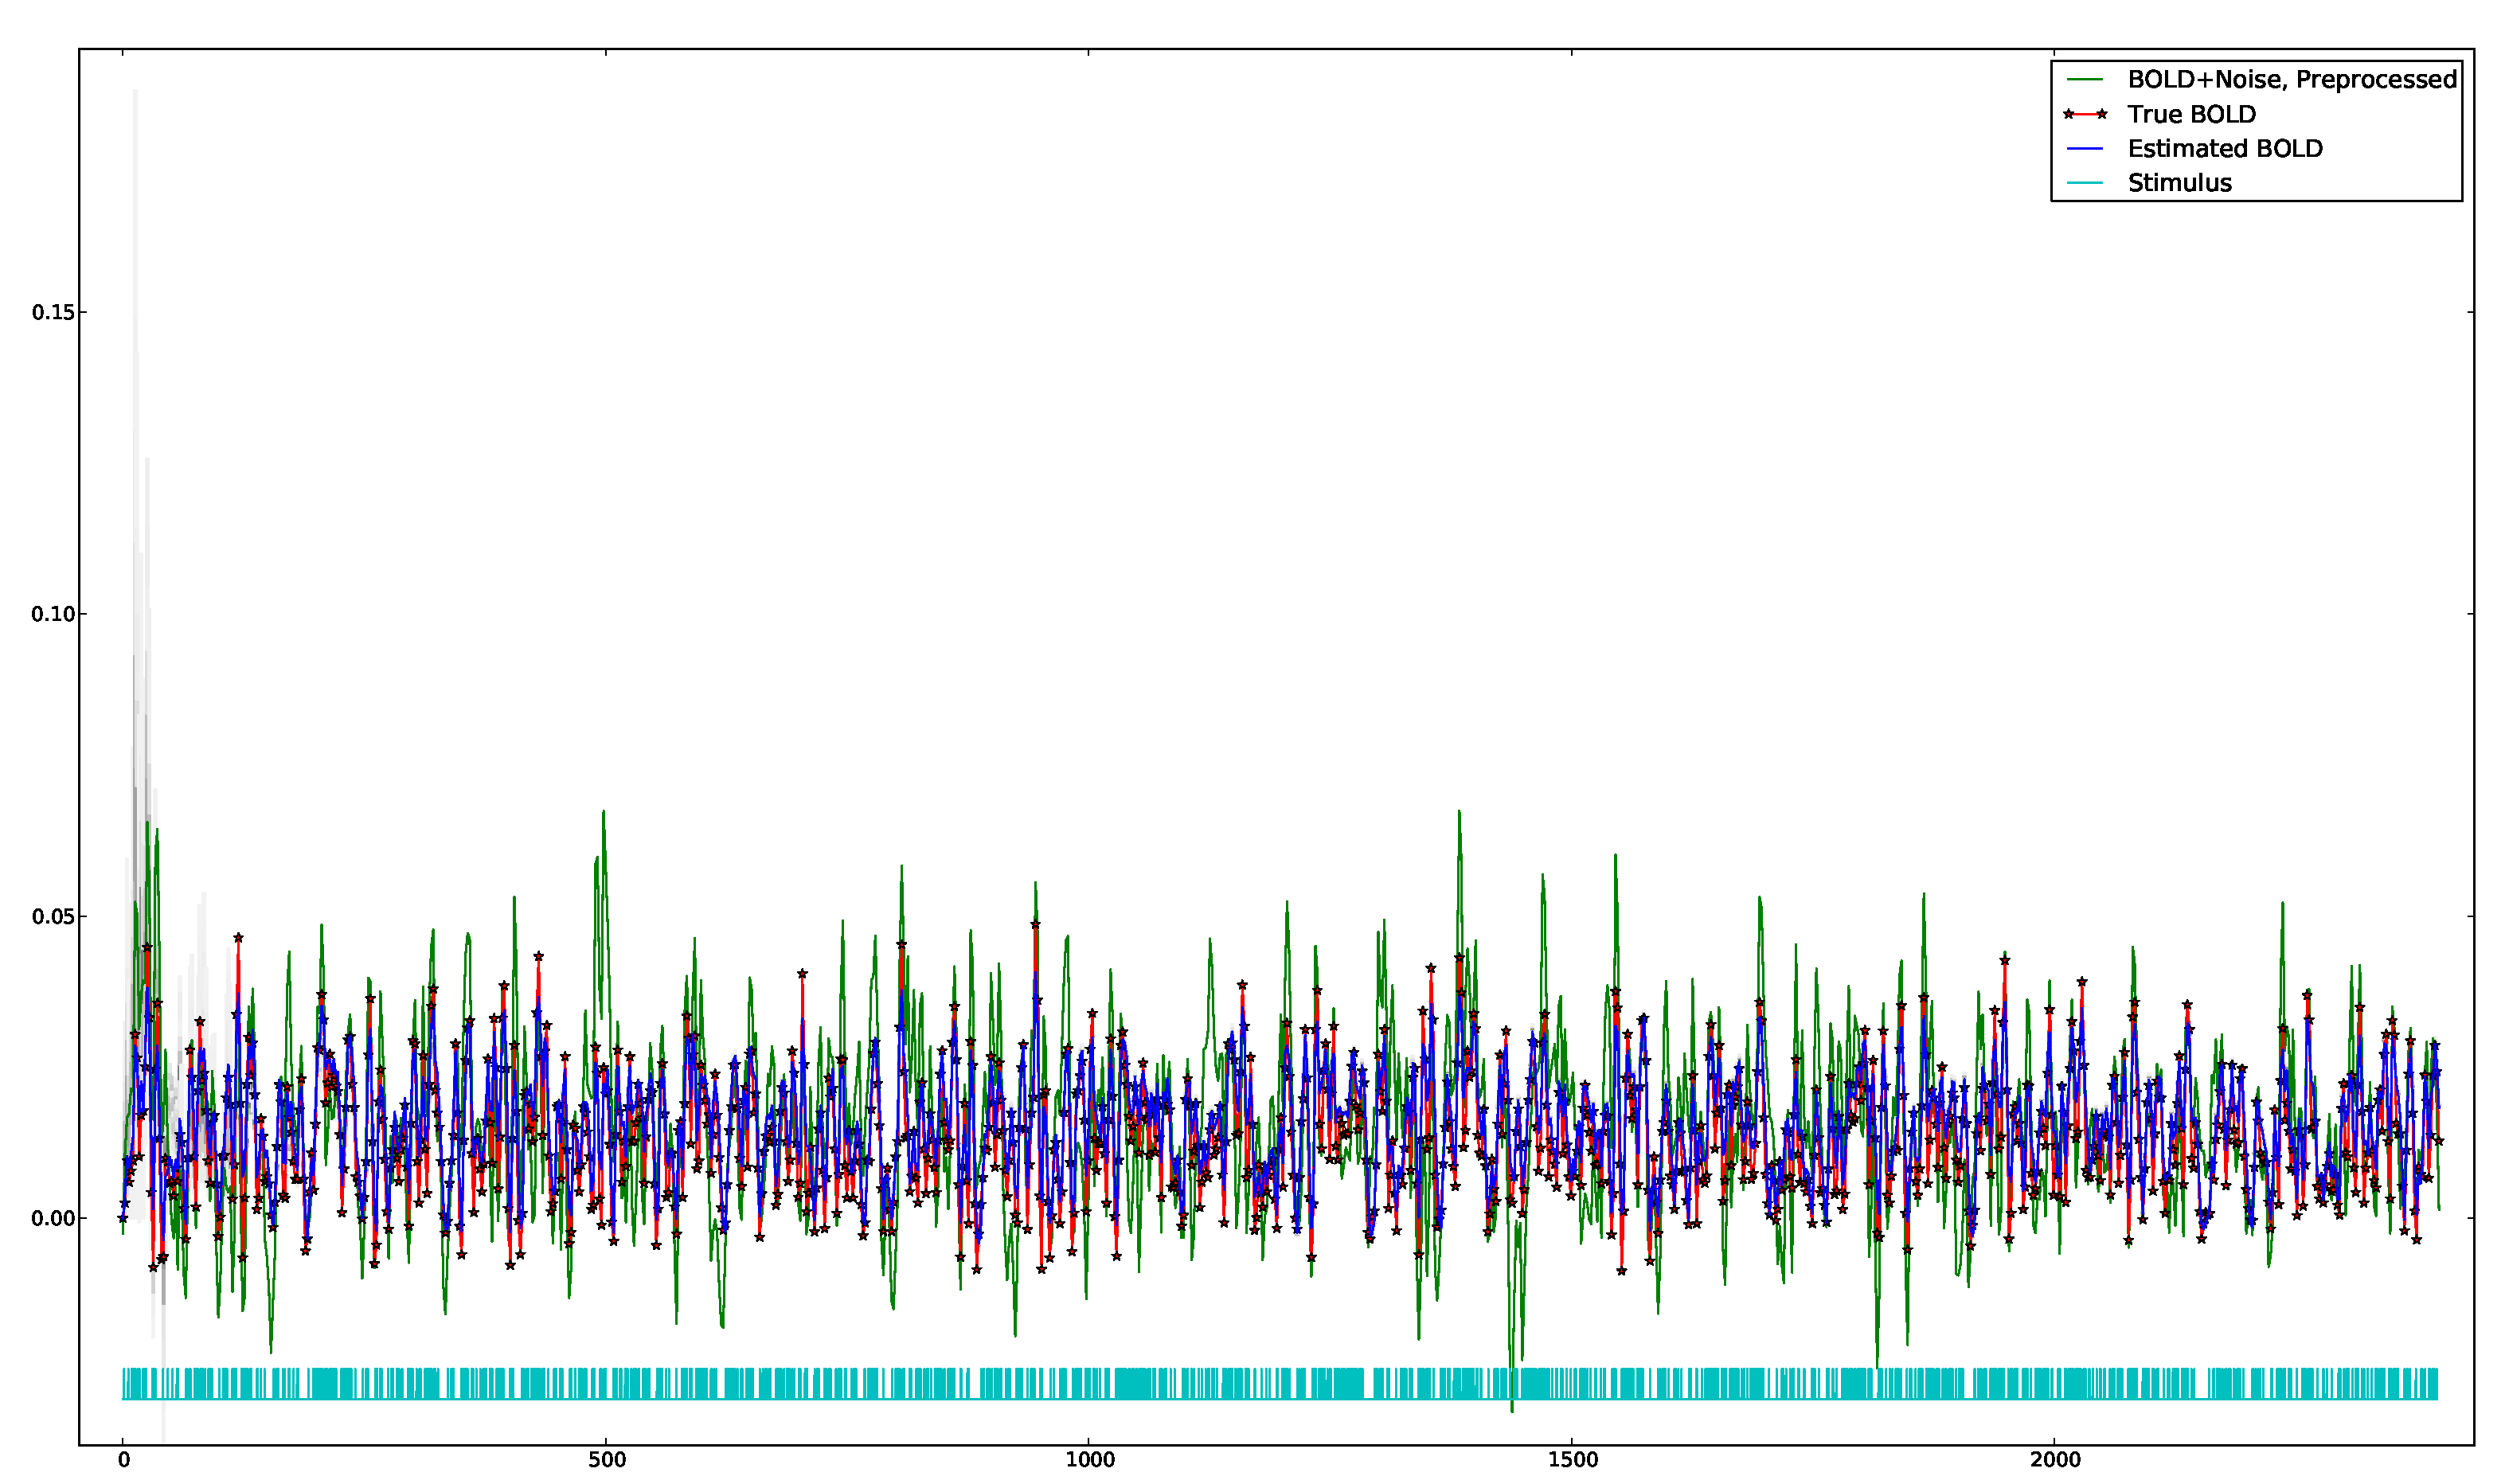
\includegraphics[clip=true,trim=1cm 0cm 0cm 0cm, width=17cm]{images/long_converge}
\caption[\ac{BOLD} estimate converging for a very long \ac{fMRI} run.]{\ac{BOLD} estimate 
converging for a 2400 second \ac{fMRI} run. Darker bars indicate
bins with more particles with BOLD estimate in that range. ($\sigma_x = 0.0005$, $\sigma_y = 0.001$)}
\label{fig:long_converge}
\end{figure}

\begin{figure}
\centering
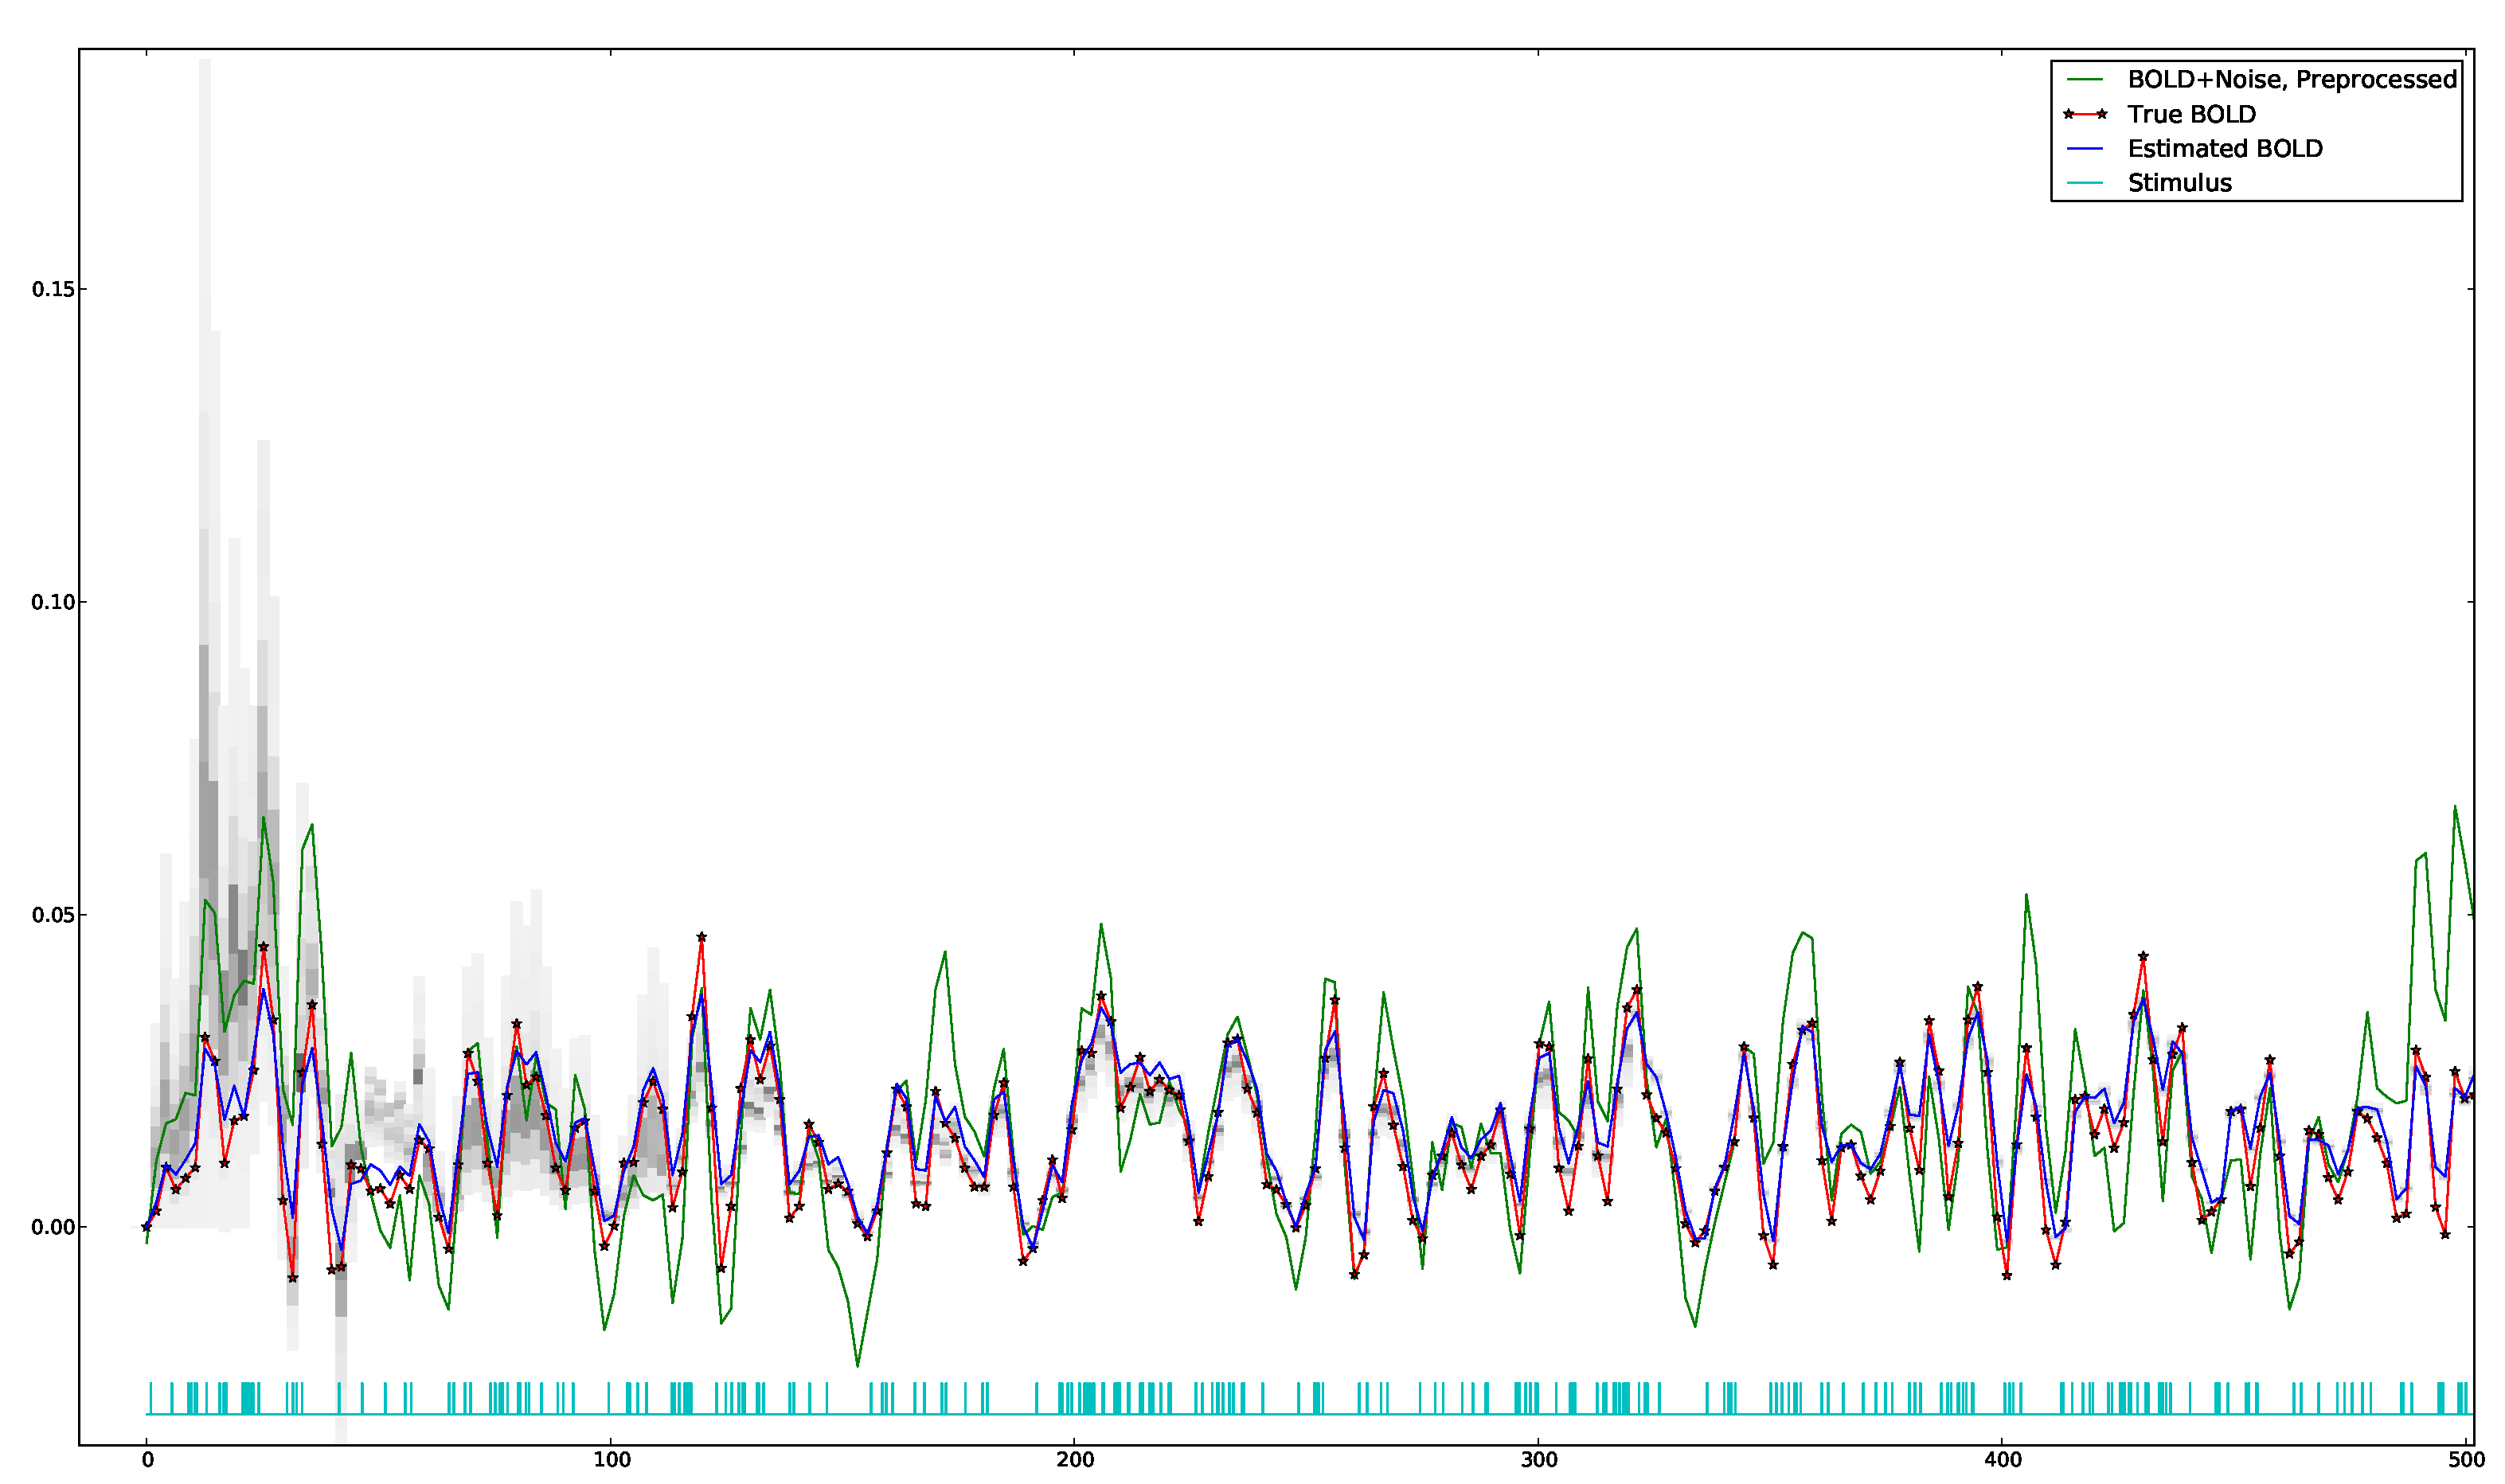
\includegraphics[clip=true,trim=1cm 0cm 0cm 0cm, width=17cm]{images/long_converge_500}
\caption[First 500 seconds of the \ac{BOLD} estimate converging for a very 
long \ac{fMRI} run.]{First 500 seconds of \ac{BOLD} estimate 
converging for a 2400 second \ac{fMRI} run. Darker bars indicate
bins with more particles with BOLD estimate in that range. ($\sigma_x = 0.0005$, $\sigma_y = 0.001$)}
\label{fig:long_converge_500}
\end{figure}

\begin{table}[t]
\begin{tabular}{|c | c  c  c  c  c  c  c |}
\hline
  & $\tau_0$ & $\alpha$ & $E_0$    & $V_0$    & $\tau_s$ & $\tau_f$ & $\epsilon$ \\
\hline
\rowcolor[gray]{.8} $\tau_0$  & 0.0004334 & 5.2e-05 & -6.95e-05 & 3.3e-06 & 0.0001628 & -2e-07 & 0.0001798 \\
$\alpha$                      & 5.2e-05 & 7.9e-06 & -6.4e-06 & 3e-07 & 1.04e-05 & -1.92e-05 & 2.58e-05 \\
\rowcolor[gray]{.8} $E_0$     & -6.95e-05 & -6.4e-06 & 1.9e-05 & -9e-07 & -4.11e-05 & -3.24e-05 & -3.92e-05 \\
$V_0$                         & 3.3e-06 & 3e-07 & -9e-07 & 1e-07 & 1.1e-06 & 9e-07 & 1e-06 \\
\rowcolor[gray]{.8} $\tau_s$  & 0.0001628 & 1.04e-05 & -4.11e-05 & 1.1e-06 & 0.0001589 & 0.0001518 & 7.88e-05 \\
$\tau_f$                      & -2e-07 & -1.92e-05 & -3.24e-05 & 9e-07 & 0.0001518 & 0.0002966 & -2.34e-05 \\
\rowcolor[gray]{.8} $\epsilon$& 0.0001798 & 2.58e-05 & -3.92e-05 & 1e-06 & 7.88e-05 & -2.34e-05 & 0.0001966 \\
\hline
\end{tabular}
\caption{Covariance matrix of the parameters at the end of \autoref{fig:long_converge}.}
\label{tab:long_cov}
\end{table}

\begin{table}[t]
\begin{tabular}{|c | c  c  c  c  c  c  c |}
\hline
  & $\tau_0$ & $\alpha$ & $E_0$    & $V_0$    & $\tau_s$ & $\tau_f$ & $\epsilon$ \\
\hline
\rowcolor[gray]{.8} $\tau_0$  & & & & & & & \\
$\alpha$                      & 0.889884 & & & & & & \\
\rowcolor[gray]{.8} $E_0$     & -0.7661395 & -0.5230723 & & & & & \\
$V_0$                         & 0.6244049 & 0.4239271 & -0.7964774 & & & & \\
\rowcolor[gray]{.8} $\tau_s$  & 0.6204843 & 0.295425 & -0.7481253 & 0.3440421 & & & \\
$\tau_f$                      & -0.0004259 & -0.3966881 & -0.4314174 & 0.1962954 & 0.6990775 & & \\
\rowcolor[gray]{.8} $\epsilon$& 0.6158116 & 0.6558179 & -0.641348 & 0.2846632 & 0.4458142 & -0.097079 & \\
\hline
\end{tabular}
\caption{Correlation of parameter estimates at the end of \autoref{fig:long_converge}.}
\label{tab:long_corr}
\end{table}

To begin the single voxel simulation; a signal using the following parameters
was generated:
$\{\tau_0 = 1.45, \alpha = 0.3, E_0 = 0.47, V_0 = 0.044, \tau_s = 1.94, \tau_f = 1.99, \epsilon = 1.8\}$.
These same parameters were used throughout this chapter. Noise
was generated based on measurement noise ($\sigma_y$) of $0.001$ and drift standard deviation
($\sigma_x$) of $0.0005$. The measurement noise as well as the steps of the drift
were taken to be Gaussian. The actual signal delivered into the particle filter
was the result of preprocessing to remove drift, as described in
\autoref{sec:Methods Preprocessing}.

To test how well the particle filter would do with plenty of data, and
determine the inherent variance in the model parameters, a very long simulation
with randomly generated impulse stimuli was created. The preprocessed time series
and the final estimate are shown in \autoref{fig:long_converge};
the final covariance matrix of the parameters is in \autoref{tab:long_cov}.
Note that even though the \ac{BOLD} response converged (\autoref{fig:long_converge},
\autoref{fig:long_converge_500}),
the parameters still have significant correlation (\autoref{tab:long_corr}).
Based on the histograms in the first 500 seconds, the parameters converged to
their final values well before the end.
Although this is only a single test, the correlation (\autoref{tab:long_corr})
of the parameters increases the probability that the parameters are
ill-defined. When the input
consists entirely of impulses, the best parameters are not one particular
set, but a joint distribution. Note that the correlation is in parameters whose priors
are completely independent. It is possible that varying the type of input could
give improved results, although informal tests did not show significant difference.
In spite of the noisy input (green line in \autoref{fig:long_converge}), the estimates
of the \ac{BOLD} were actually very close to the true (noise-free) \ac{BOLD} signal.

%LOW NOISE SECTION, with a signal
\subsection{Simulation with Low Noise}
\label{sec:SimLowNoise}
%tests had noise of $ \{\sigma_y = .01, \sigma_x = .005\} $, where $\sigma_y$ is the
%measurement noise, and $\sigma_x$ is the wiener step size. Both signals used the
%parameters .
%The particle filter used the parameters defined in \autoref{tab:Prior} (\autoref{sec:PriorDistrib}),
%thus the particle filter was not centered over the correct values.
\begin{figure}
\centering
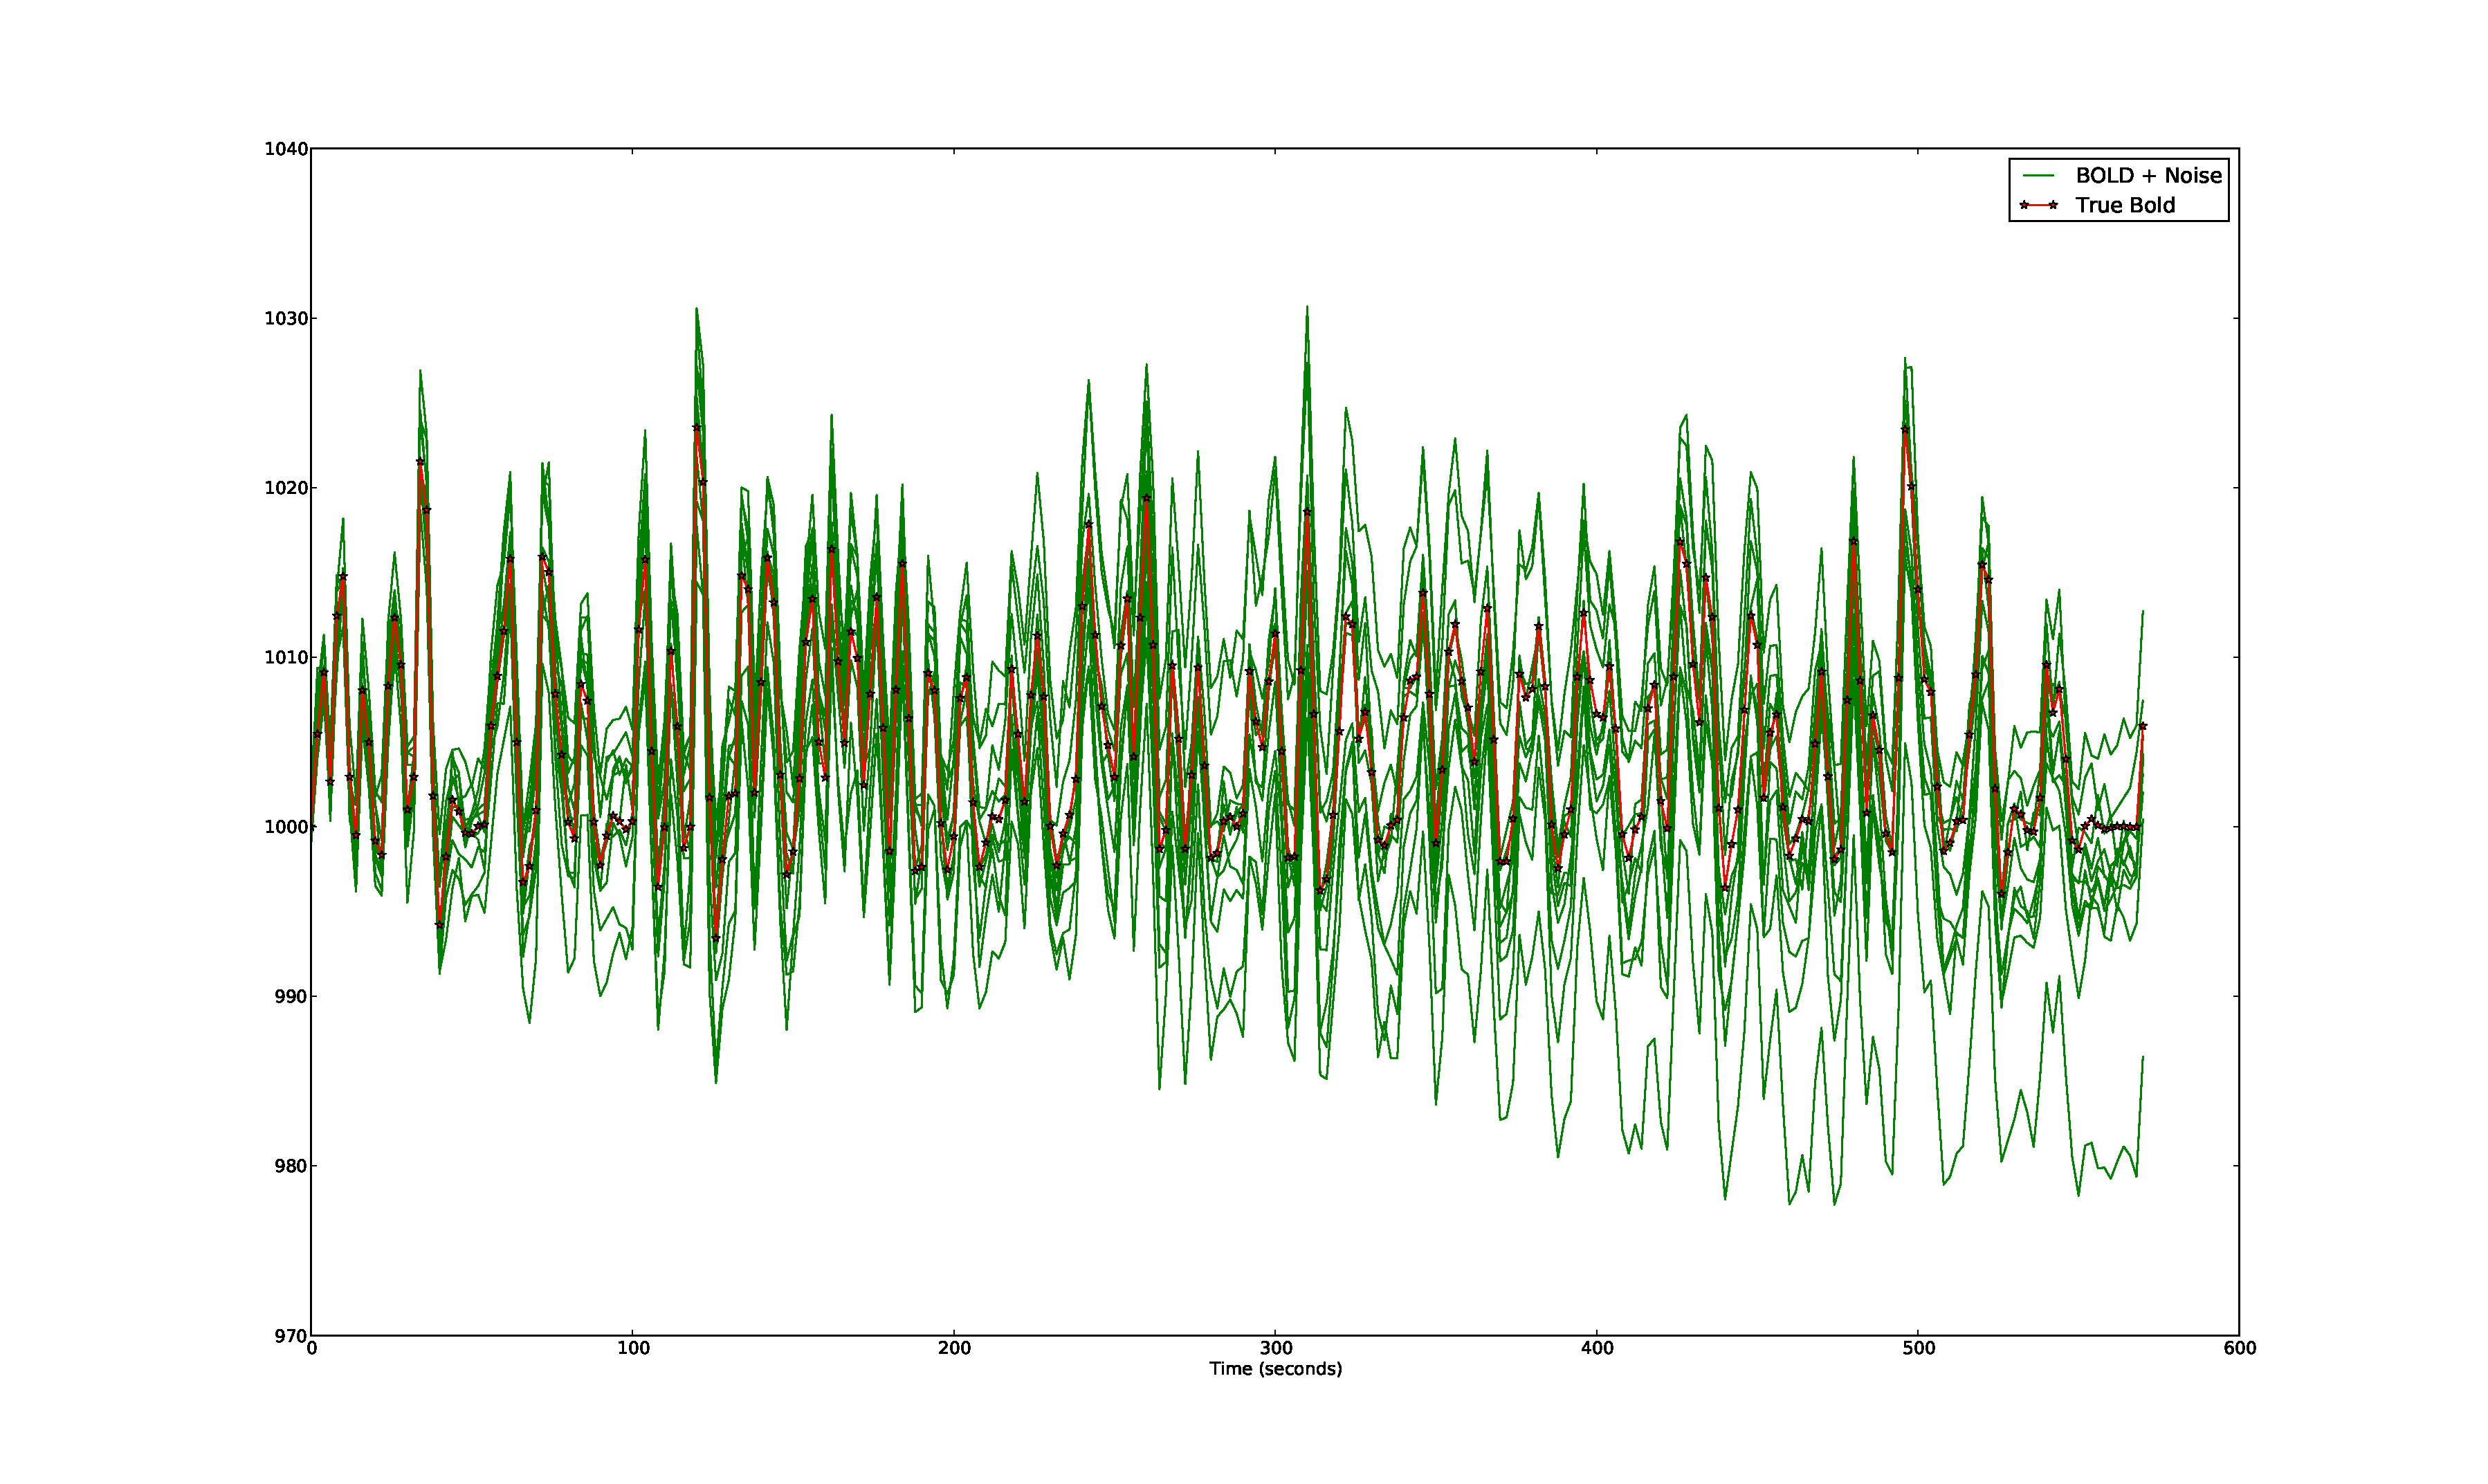
\includegraphics[clip=true,trim=6cm 2cm 5cm 3.5cm,width=15cm]{images/realization_lownoise}
\caption[Simulated Signal with Low Noise/Drift]
{Simulated signals with different noise realizations compared to true
signal. ($\sigma_x = 0.0005$, $\sigma_y = 0.001$)}
\label{fig:LowNoiseRealization}
\end{figure}

\begin{figure}
\centering
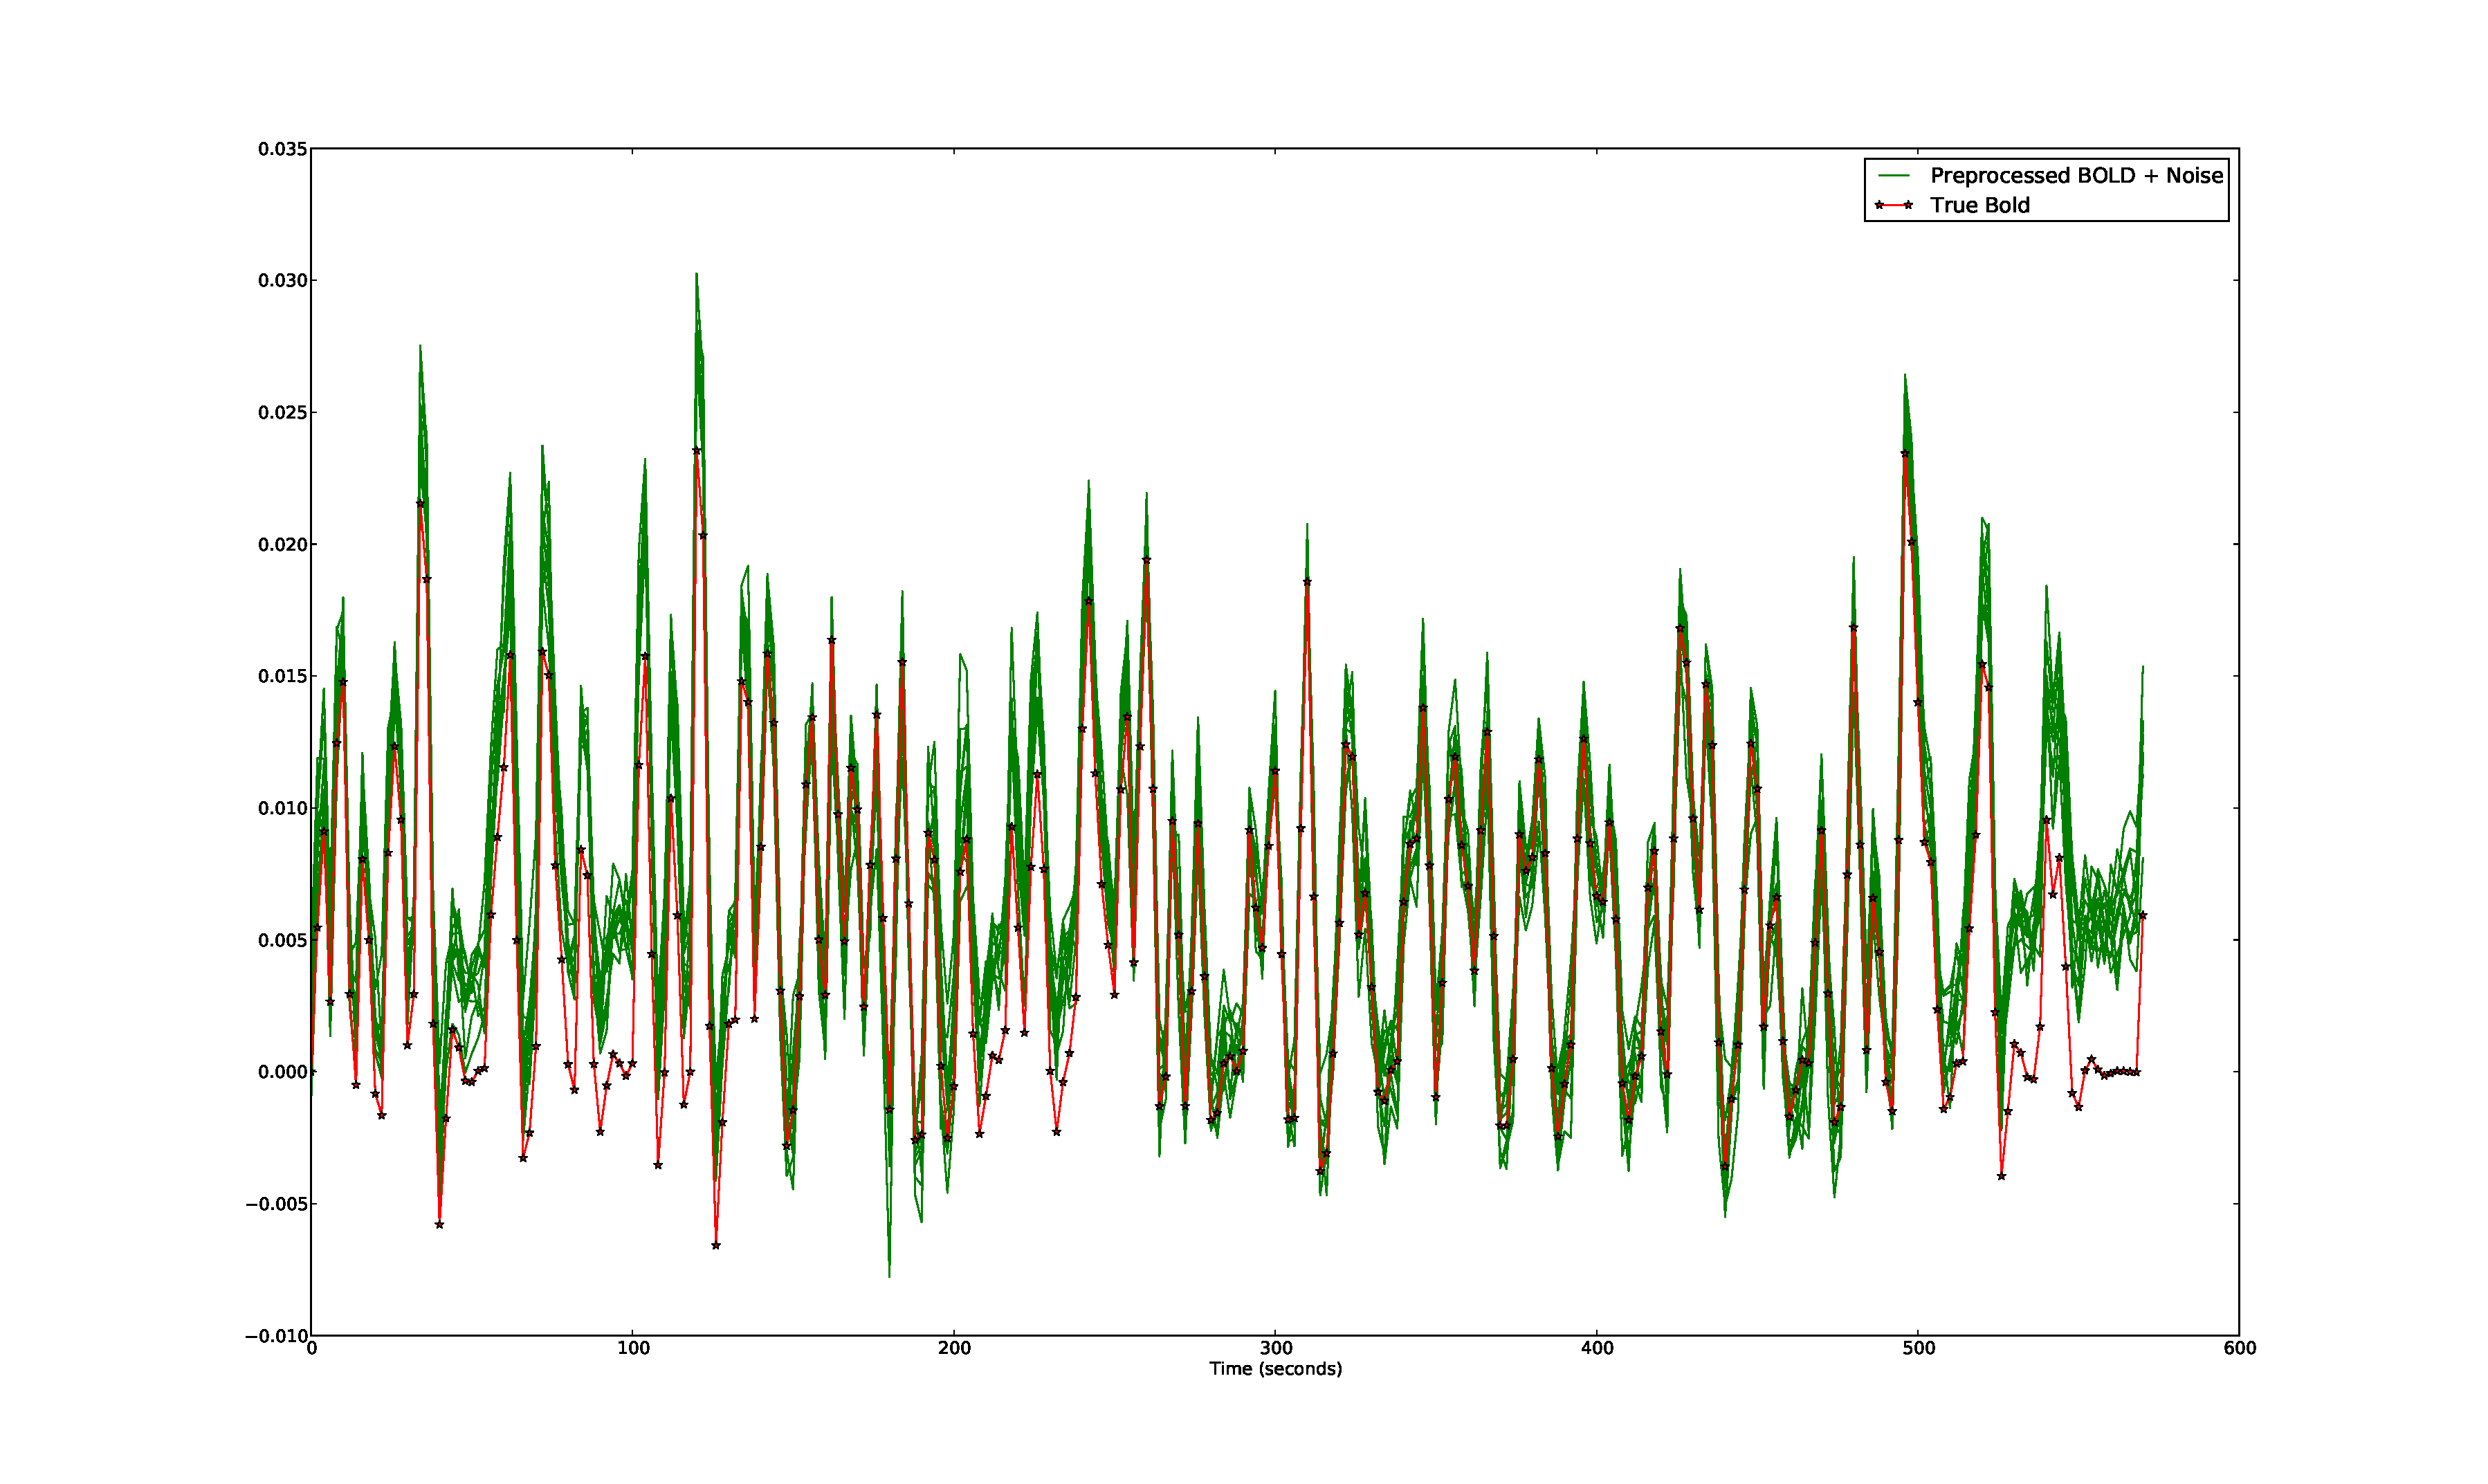
\includegraphics[clip=true,trim=6cm 2cm 5cm 3.5cm,width=15cm]{images/preprocessed_lownoise}
\caption[Preprocessed Signal with Low Noise/Drift]
{Results of preprocessing compared to the true signal. 
 Knots of spline placed every 20 measurements.
 ($\sigma_x = 0.0005$, $\sigma_y = 0.001$)}
\label{fig:PreprocessedLowNoise}
\end{figure}

\begin{figure}
\centering
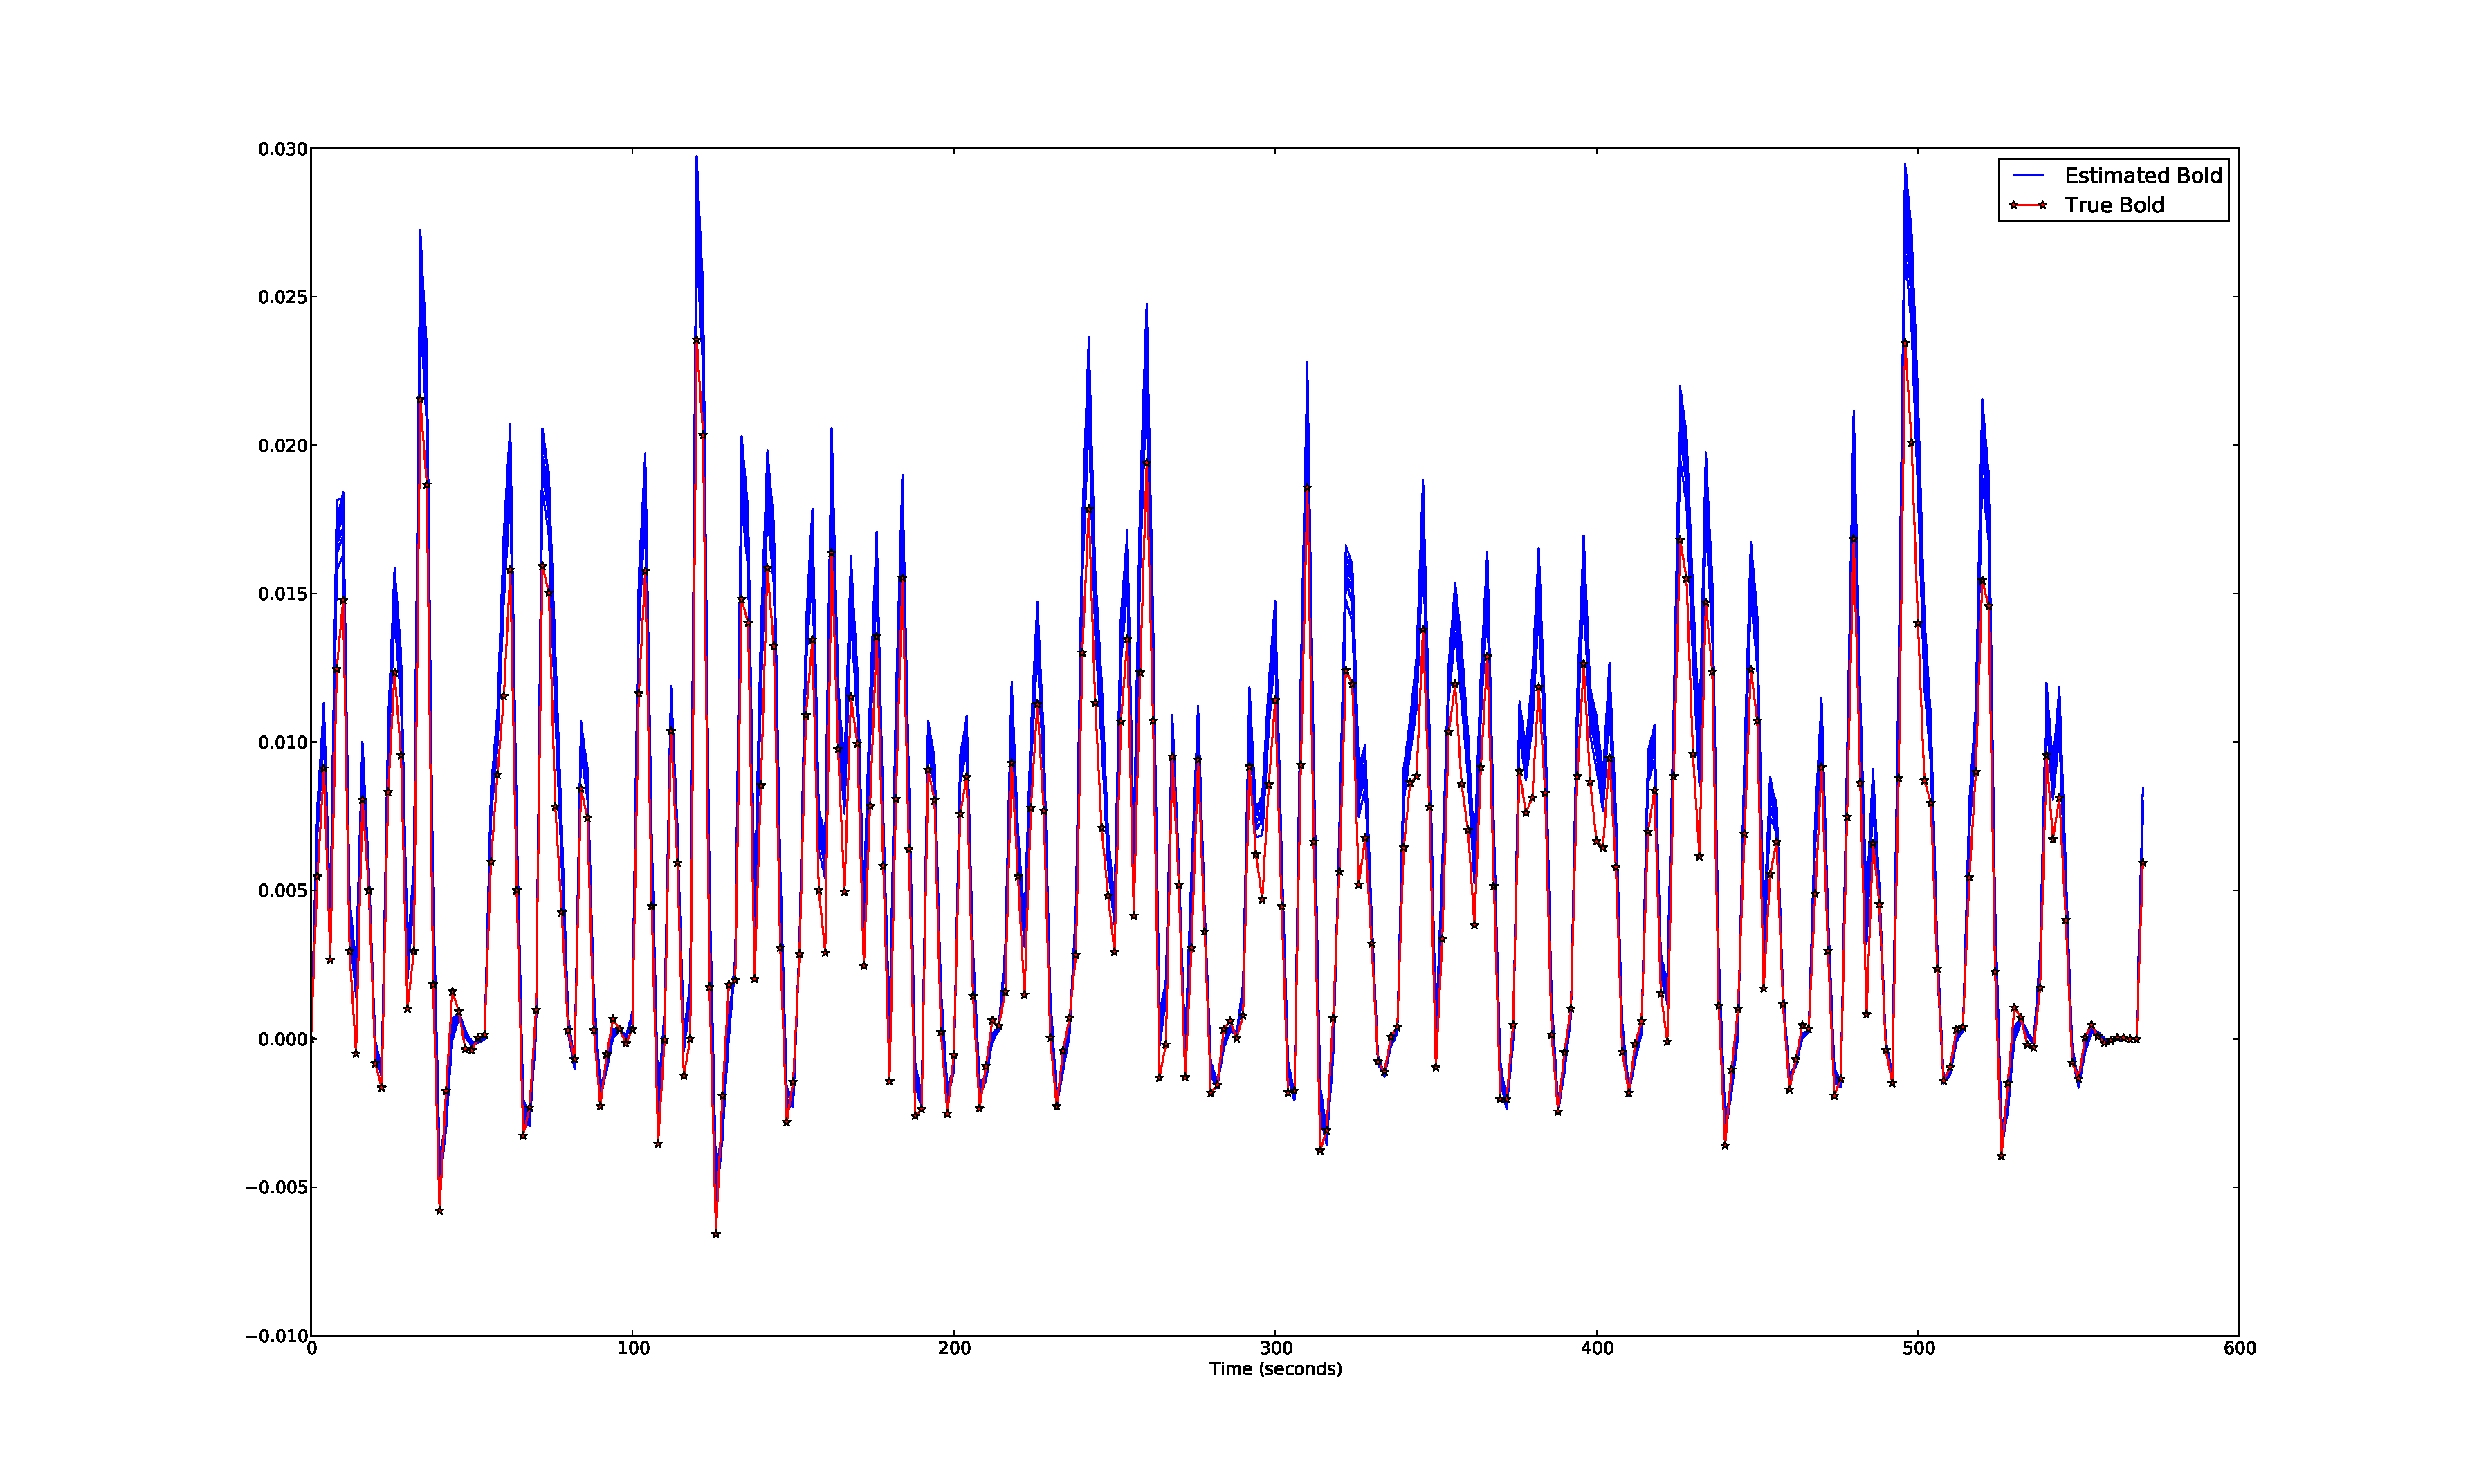
\includegraphics[clip=true,trim=6cm 2cm 5cm 3.5cm,width=15cm]{images/comparison_lownoise}
\caption[Results with Low Noise/Drift]
{Results of the particles filter with preprocessed signals from \autoref{fig:PreprocessedLowNoise}
as input.}
\label{fig:FitComparisonLowNoise}
\end{figure}

\begin{table}[t]
\centering
\begin{tabular}{|c | c | c | c | c | c | c | c | c | c |}
\hline
$\tau_0$ & $\alpha$ & $E_0$    & $V_0$    & $\tau_s$ & $\tau_f$ & $\epsilon$  & $ \sum \tau $ & \acs{RMSR} & \acs{RMSE} \\
\hline
\rowcolor[gray]{.8}
1.45 & 0.3 & 0.47 & 0.044 & 1.94 & 1.99 & 1.8  & 5.38 &  & \\
\hline
\hline
1.2221 & 0.3449 & 0.3346 & 0.0714 & 1.6045 & 2.2753 & 1.5945 & 5.1019 &  0.003211  & 0.00224\\
1.3749 & 0.3318 & 0.3630 & 0.0733 & 1.6408 & 2.1030 & 1.5763 & 5.1187 &  0.003055  & 0.00223\\
1.1660 & 0.3221 & 0.3406 & 0.0822 & 1.6477 & 2.3535 & 1.2452 & 5.1672 &  0.003289  & 0.00205\\
1.2318 & 0.3271 & 0.3403 & 0.0796 & 1.6270 & 2.1852 & 1.3033 & 5.0439 &  0.002847  & 0.00147\\
1.1832 & 0.3179 & 0.3472 & 0.0821 & 1.5496 & 2.2912 & 1.2782 & 5.0240 &  0.003006  & 0.00213\\
1.1424 & 0.334  & 0.3473 & 0.0737 & 1.6221 & 2.2908 & 1.4025 & 5.0553 &  0.002833  & 0.00184\\
1.3004 & 0.3596 & 0.3564 & 0.0768 & 1.5641 & 2.1323 & 1.6034 & 4.9968 &  0.003028  & 0.00255\\
1.2401 & 0.3460 & 0.3398 & 0.0891 & 1.6499 & 2.2366 & 1.2900 & 5.1265 &  0.003044  & 0.00238\\
1.1709 & 0.3274 & 0.3464 & 0.0826 & 1.5373 & 2.2826 & 1.3783 & 4.9909 &  0.003345  & 0.0027 \\
1.1897 & 0.3434 & 0.3355 & 0.0798 & 1.5358 & 2.3075 & 1.4277 & 5.0330 &  0.003175  & 0.00244\\
1.184 &  0.3405 & 0.3502 & 0.0892 & 1.6103 & 2.2793 & 1.1645 & 5.0735 &  0.002889  & 0.00188\\
\hline                                                                               
1.2187 & 0.3359 & 0.3456 & 0.0800 & 1.599 & 2.2488 & 1.3876 & 5.0665 & 0.003066     & 0.00217\\
\hline
\end{tabular}
\caption{Estimated Parameters on 11 different runs with low noise. First row is the true value, 
last is the average. $\sum \tau$ is the sum of the estimated time constants.}
\label{tab:LowNoiseResults}
\end{table}

\begin{figure}
\subfigure
{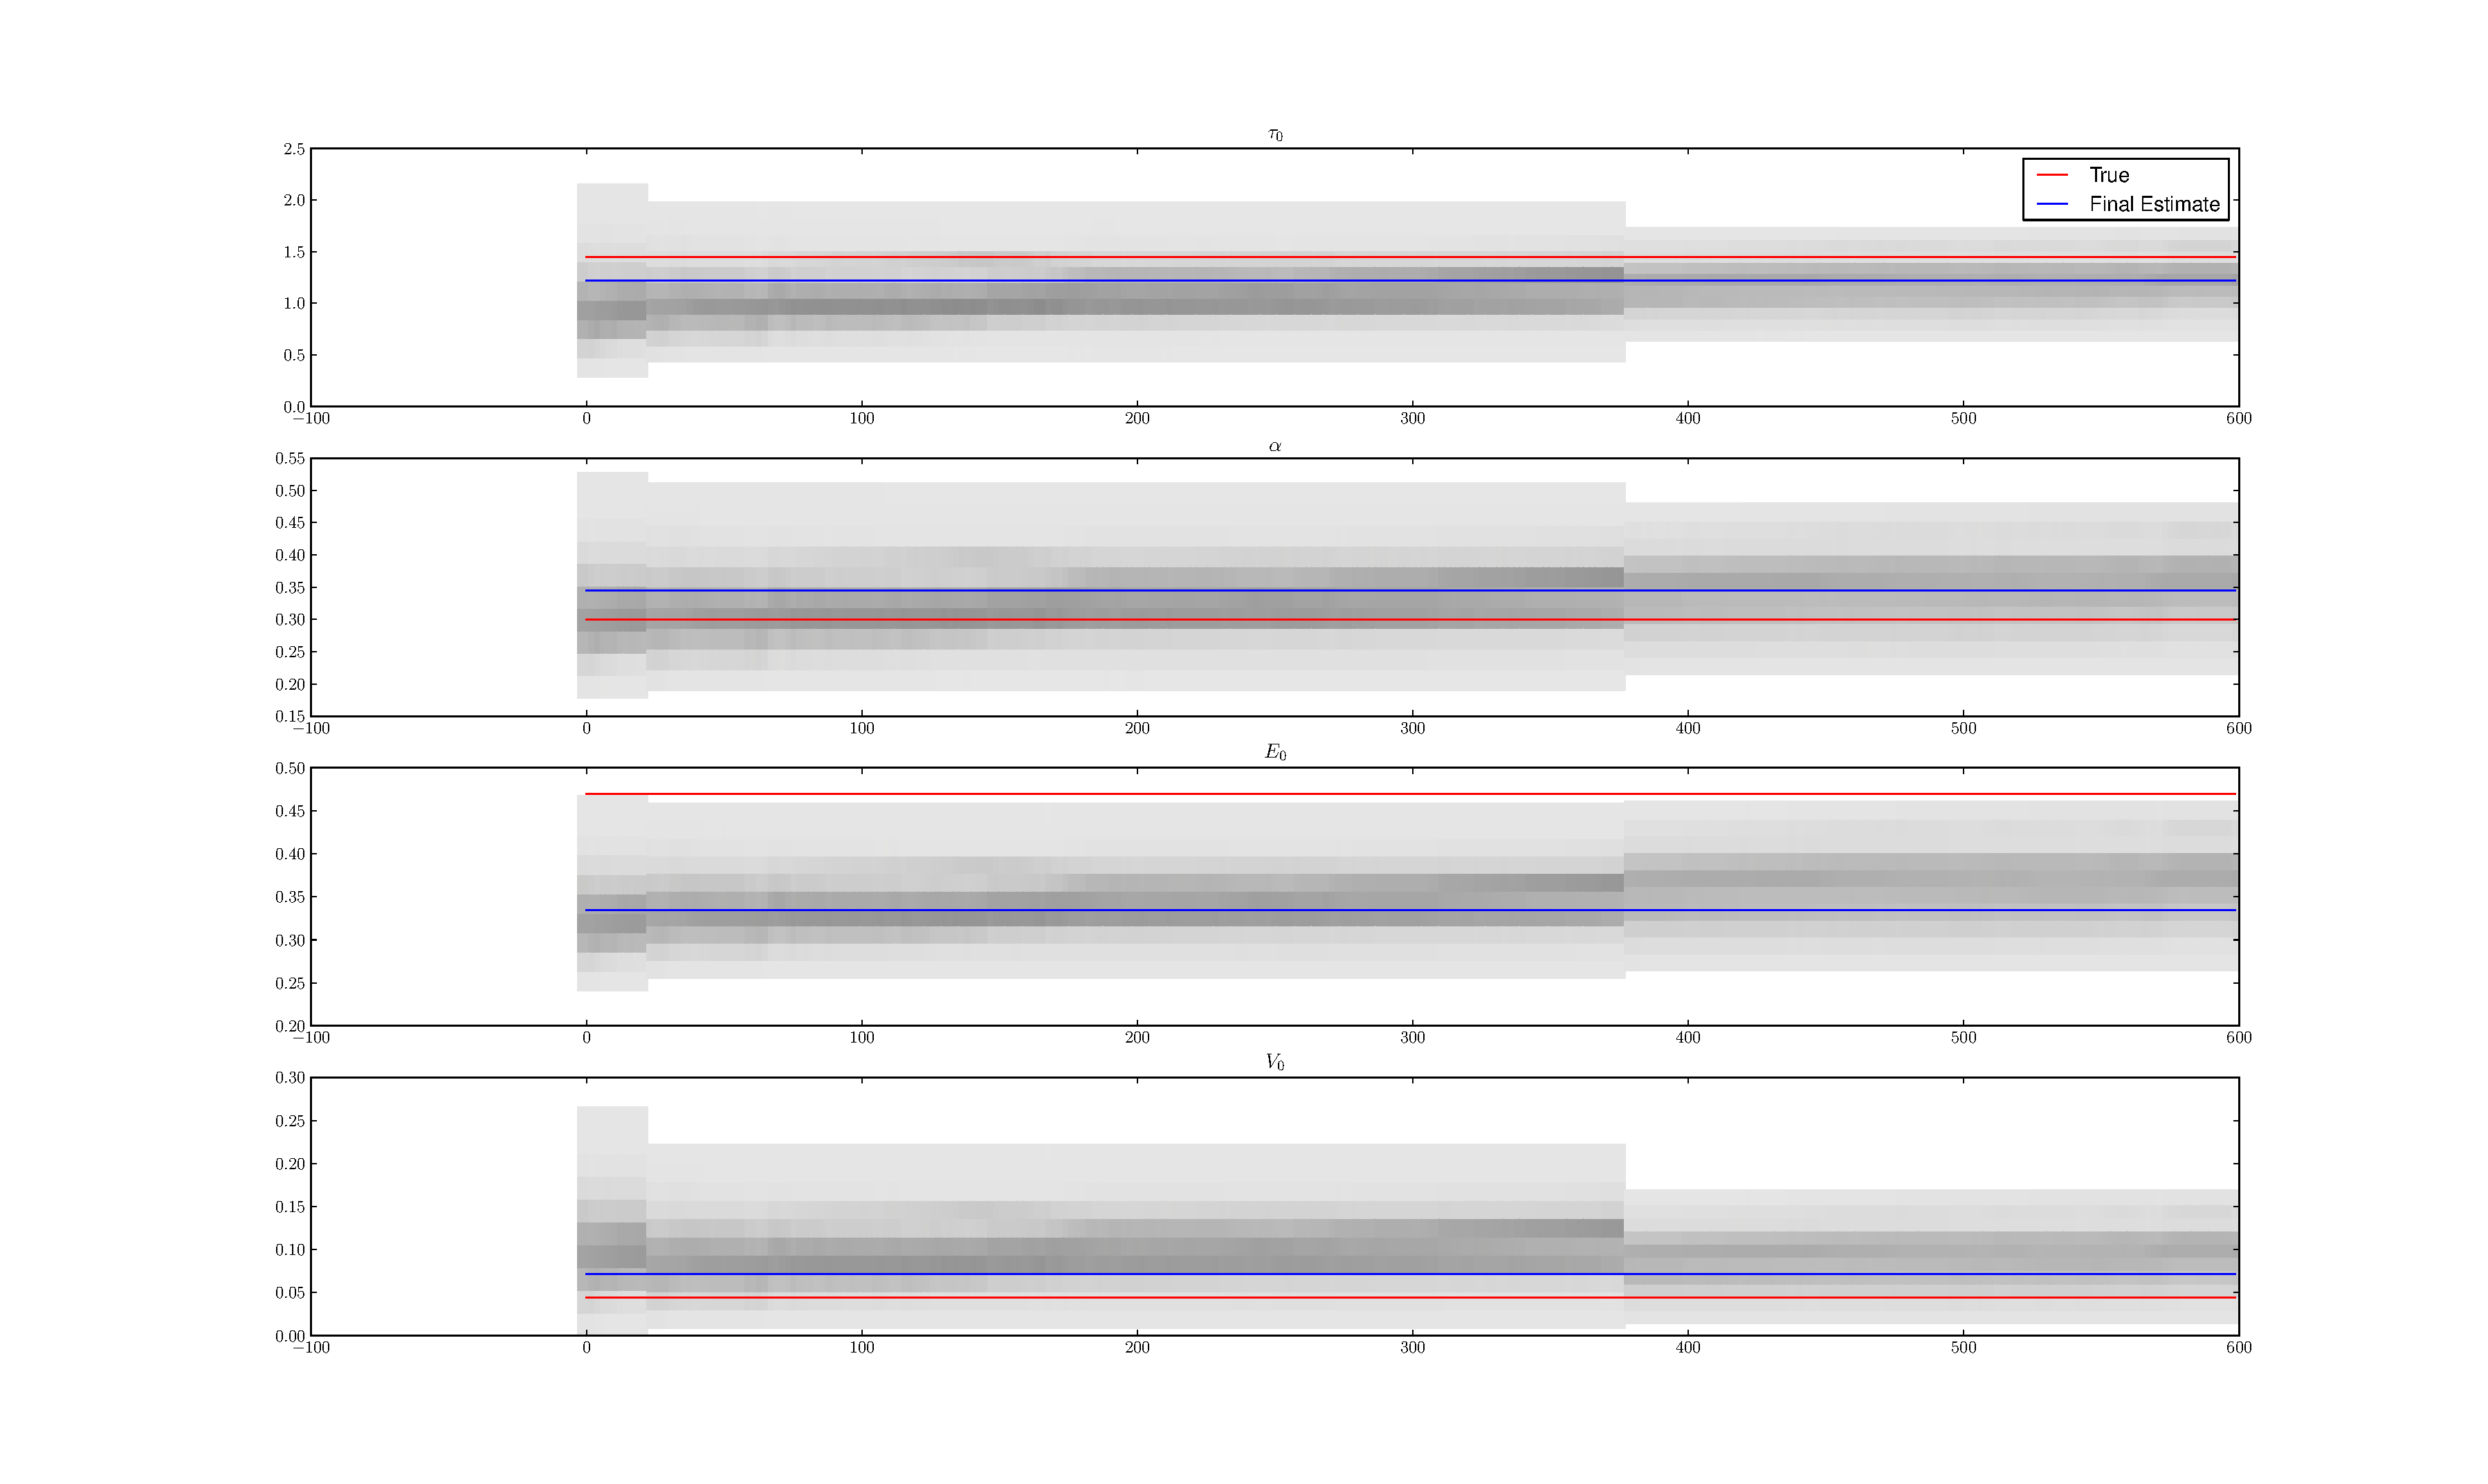
\includegraphics[clip=true,trim=7cm 3cm 6cm 3cm, width=\textwidth]{images/converge_lownoise1}}
\subfigure
{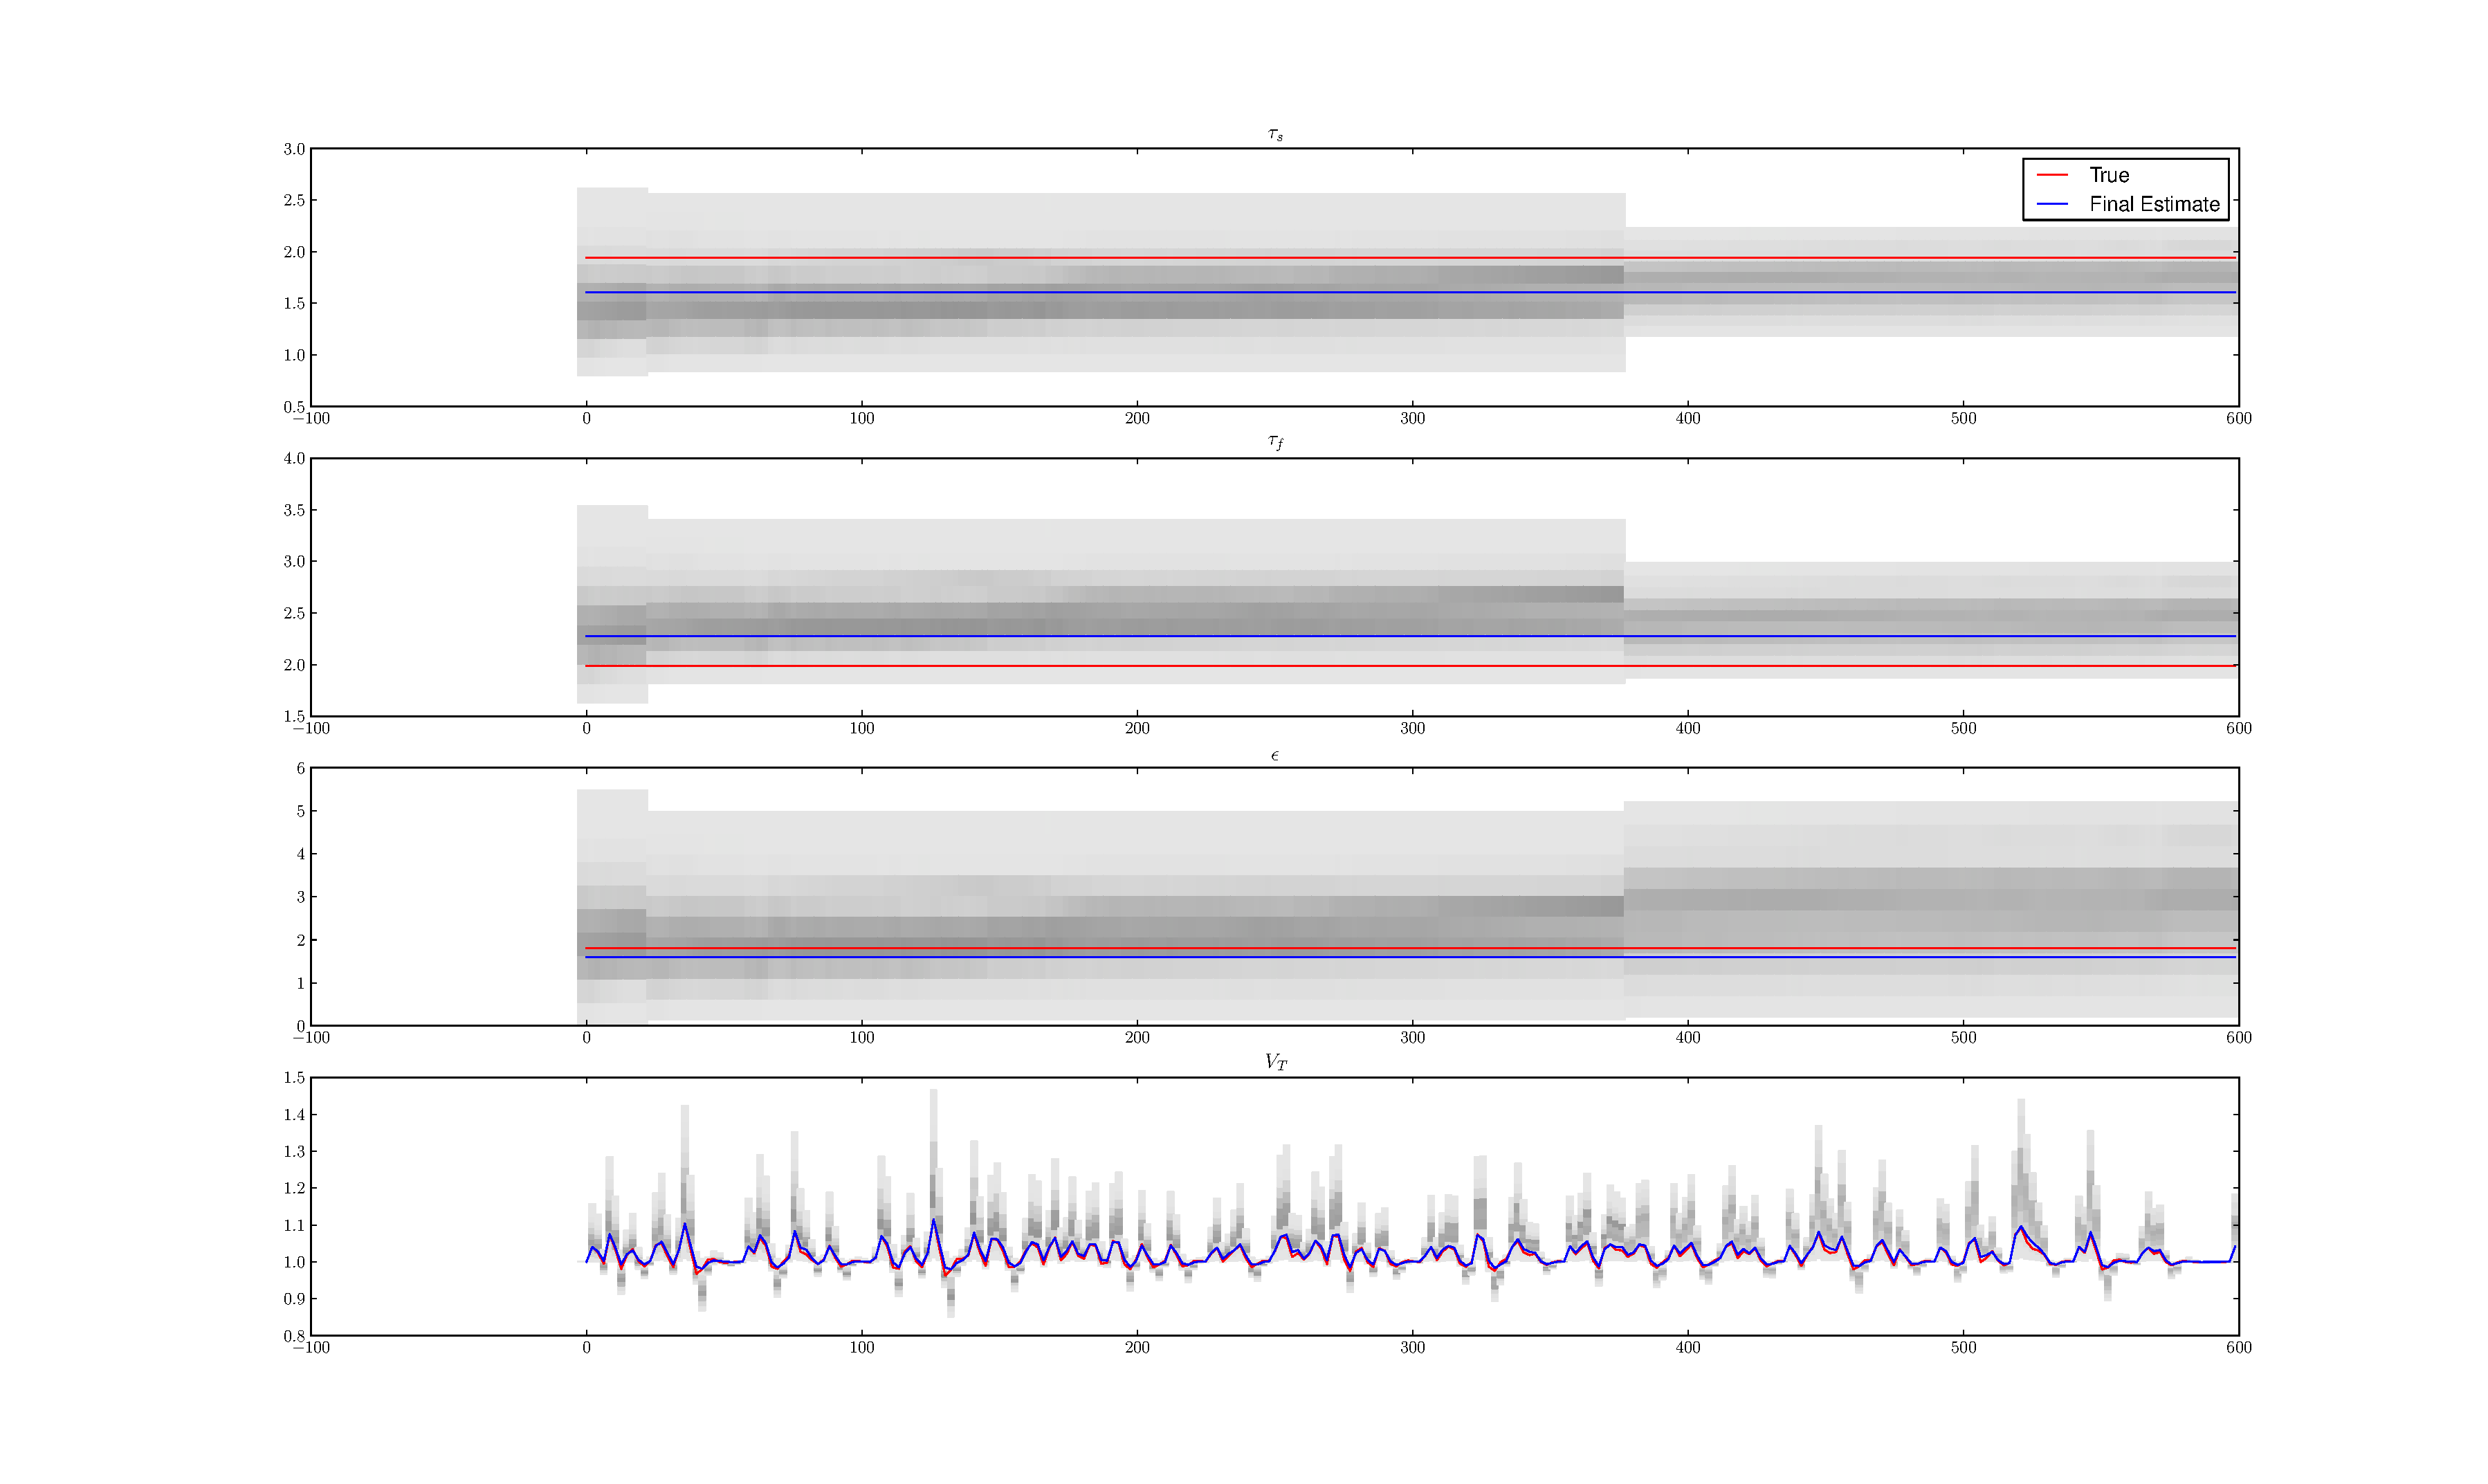
\includegraphics[clip=true,trim=7cm 3cm 6cm 3cm, width=\textwidth]{images/converge_lownoise2}}
\end{figure}

\begin{figure}
\subfigure
{\label{fig:LowNoiseHistc} 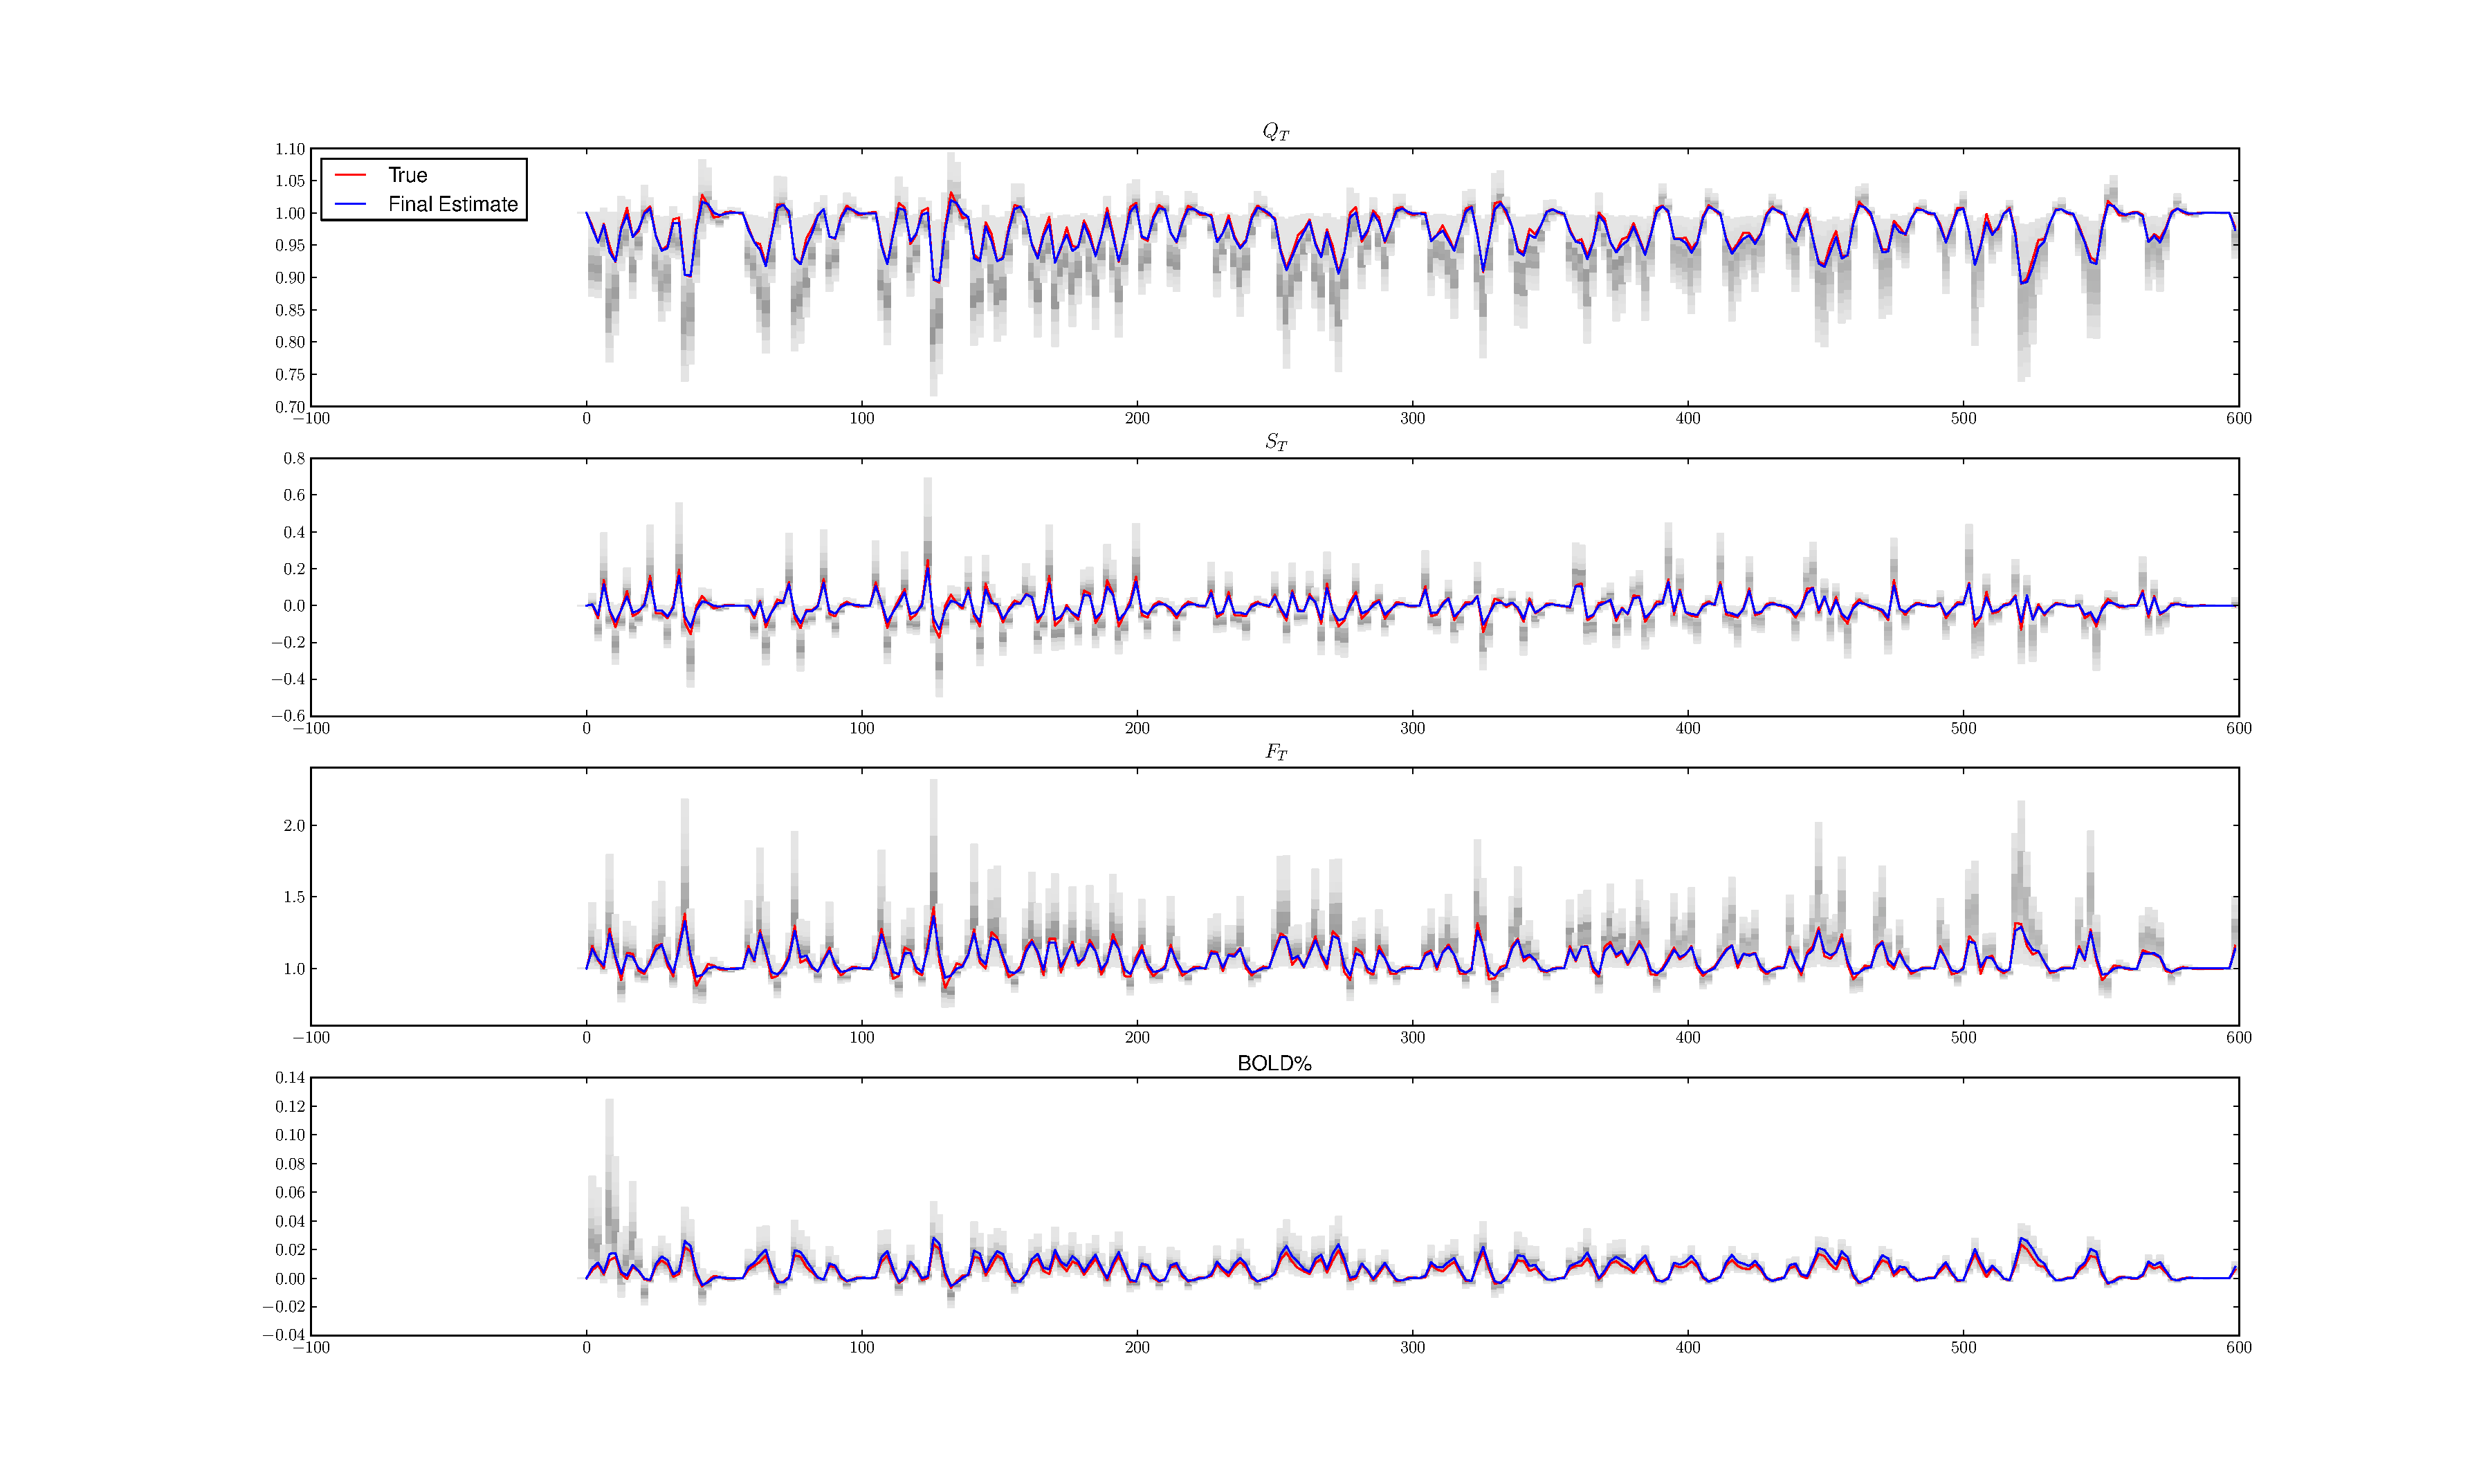
\includegraphics[clip=true,trim=7cm 3cm 6cm 3cm, width=\textwidth]{images/converge_lownoise3}}
\caption[Convergence of the parameters from the first run of \autoref{tab:LowNoiseResults}.]
{Convergence of the parameters from the first run of \autoref{tab:LowNoiseResults}. 
Order of estimates: $\tau_0, \alpha, E_0, V_0, \tau_s, \tau_f, \epsilon, v,
q, s, f, BOLD$.  The bars represent
a histogram, where darker bars indicate more particles with parameters in that bin. The red 
line is the parameter used to generate the true signal, blue line is the final mean of the
particles.}
\label{fig:LowNoiseHist}
\end{figure}

The following tests all use less data (shorter sequences), on par with
the average length of an \ac{fMRI} session. For this low noise case
$(\sigma_y = 0.001,\ \sigma_x = .0005)$, the eleven realizations are shown in
\autoref{fig:LowNoiseRealization}.
The bias introduced into the signal by preprocessing
could have some effect on the resulting fit; thus the preprocessed signal is compared
to the true \ac{BOLD} signal in \autoref{fig:PreprocessedLowNoise}.
Overall, \autoref{fig:PreprocessedLowNoise} shows that the preprocessing was
effective at removing trends, although the spline did leave some noise 
structure toward the end (\autore{fig:LowNoiseRealization}). This slight 
drift effect was caused by the final median being well above the base
level.
At several time points the particle filter successfully filtered the input
(\autoref{fig:FitComparisonLowNoise}).
For instance, in the last 30 seconds
the estimates stay flat in spite of the preprocessed data drifting off. By
this point, the algorithm had converged sufficiently to prevent such inexplicable movement.
A similar circumstance occurs at around 100 seconds in. A combination of
noise and preprocessing biased the results toward a peak signal above the true peaks.
The final parameter sets are shown in
\autoref{tab:LowNoiseResults}.

For the purpose of quantifying the quality of fit, the 
\ac{RMSR} was used:
\begin{equation}
\text{RMSR} = \sqrt{\frac{1}{N}\sum (\hat{y}_k - y_k)^2}
\end{equation}
where $\hat{y}_k$ is the estimated output at time $k$ and $y_k$ is the 
preprocessed output
sampled at time $k$. Note the subtle distinction between this and
the \ac{RMSE}:
\begin{equation}
\text{RMSE} = \sqrt{\frac{1}{N}\sum (\hat{y}_k - Y_k)^2}
\end{equation}
where $\hat{y}_k$ is the estimated output, and $Y_k$ is the underlying 
(free of noise) signal. 

There are a few important results in the final parameter estimates (which
are the mean of the particle filter's posterior distribution). First, the time constants vary
greatly across
runs, yet the sum of the individual time constants
($\tau_f$, $\tau_s$ and $\tau_0$) was more consistent. On average the
time constants fell short of the true time constant. This could be a limitation
based on the prior distribution (which notably had an initial mean below the true values)
or it could be that other parameters compensated. It is also possible that the output is insensitive
to small differences in the time constants.
The convergence of the first run in \autoref{tab:LowNoiseResults}
demonstrates the migration of parameters through the run. In spite of the
significant differences in parameter estimates, the estimated \ac{BOLD}
consistently performed well
(\autoref{fig:FitComparisonLowNoise}).


%The large variation of $V_0$ are also interesting, although as the final
%covariance matrix of the first run shows, there is a significant correlation between $\epsilon$ and $V_0$.
%In general, with even a small amount of noise, parameters are ill defined. Thus at
%least for this set of stimuli the parameters are not uniquely identifiable.
%
%The covariance matrix (\autoref{tab:CovSim}) provides a great deal of insight into
%the way parameters evolve in the particle filter. The number of
%covariance elements that exceed the variance elements indicates the
%significant interplay between parameters. Every single parameters, including $\alpha$,
%has a non-zero covariance. Why $\alpha$ and $\epsilon$ would be positively related
%is the most interesting element. The answer of how exactly each parameter
%compensates for other parameters is complex.  Notice the covariance of $\tau_f$ and $\tau_0$
%is $-0.019$ whereas the variance of $\tau_0$ and $\tau_f$ are $0.019$ and $0.04$ respectively.
%%stopped here
%As Clearly there is some measure of ill-defined behavior between the different time-constants, which is to
%be expected given the number steps before a stimuli affects the output.
%The convergence properties of the first run in \autoref{tab:LowNoiseResults}
%demonstrates the migration of parameters to match the estimates. Given the relatively high
%variance of parameters, its likely that more measurements or perhaps more variation
%in the stimuli could further differentiate the parameters. Its also notable that
%the final mean of the parameters may not be the best point estimator, and that perhaps
%using the mode would be a better way to estimate the output. Regardless, the time series'
%generated from the estimated mean seems to match the correct signal very well
%(\autoref{fig:FitComparisonLowNoise}).

%HIGH NOISE SECTION, with a signal
\subsection{Simulation with High Noise}
\label{sec:SimHighNoise}
%\begin{figure}
%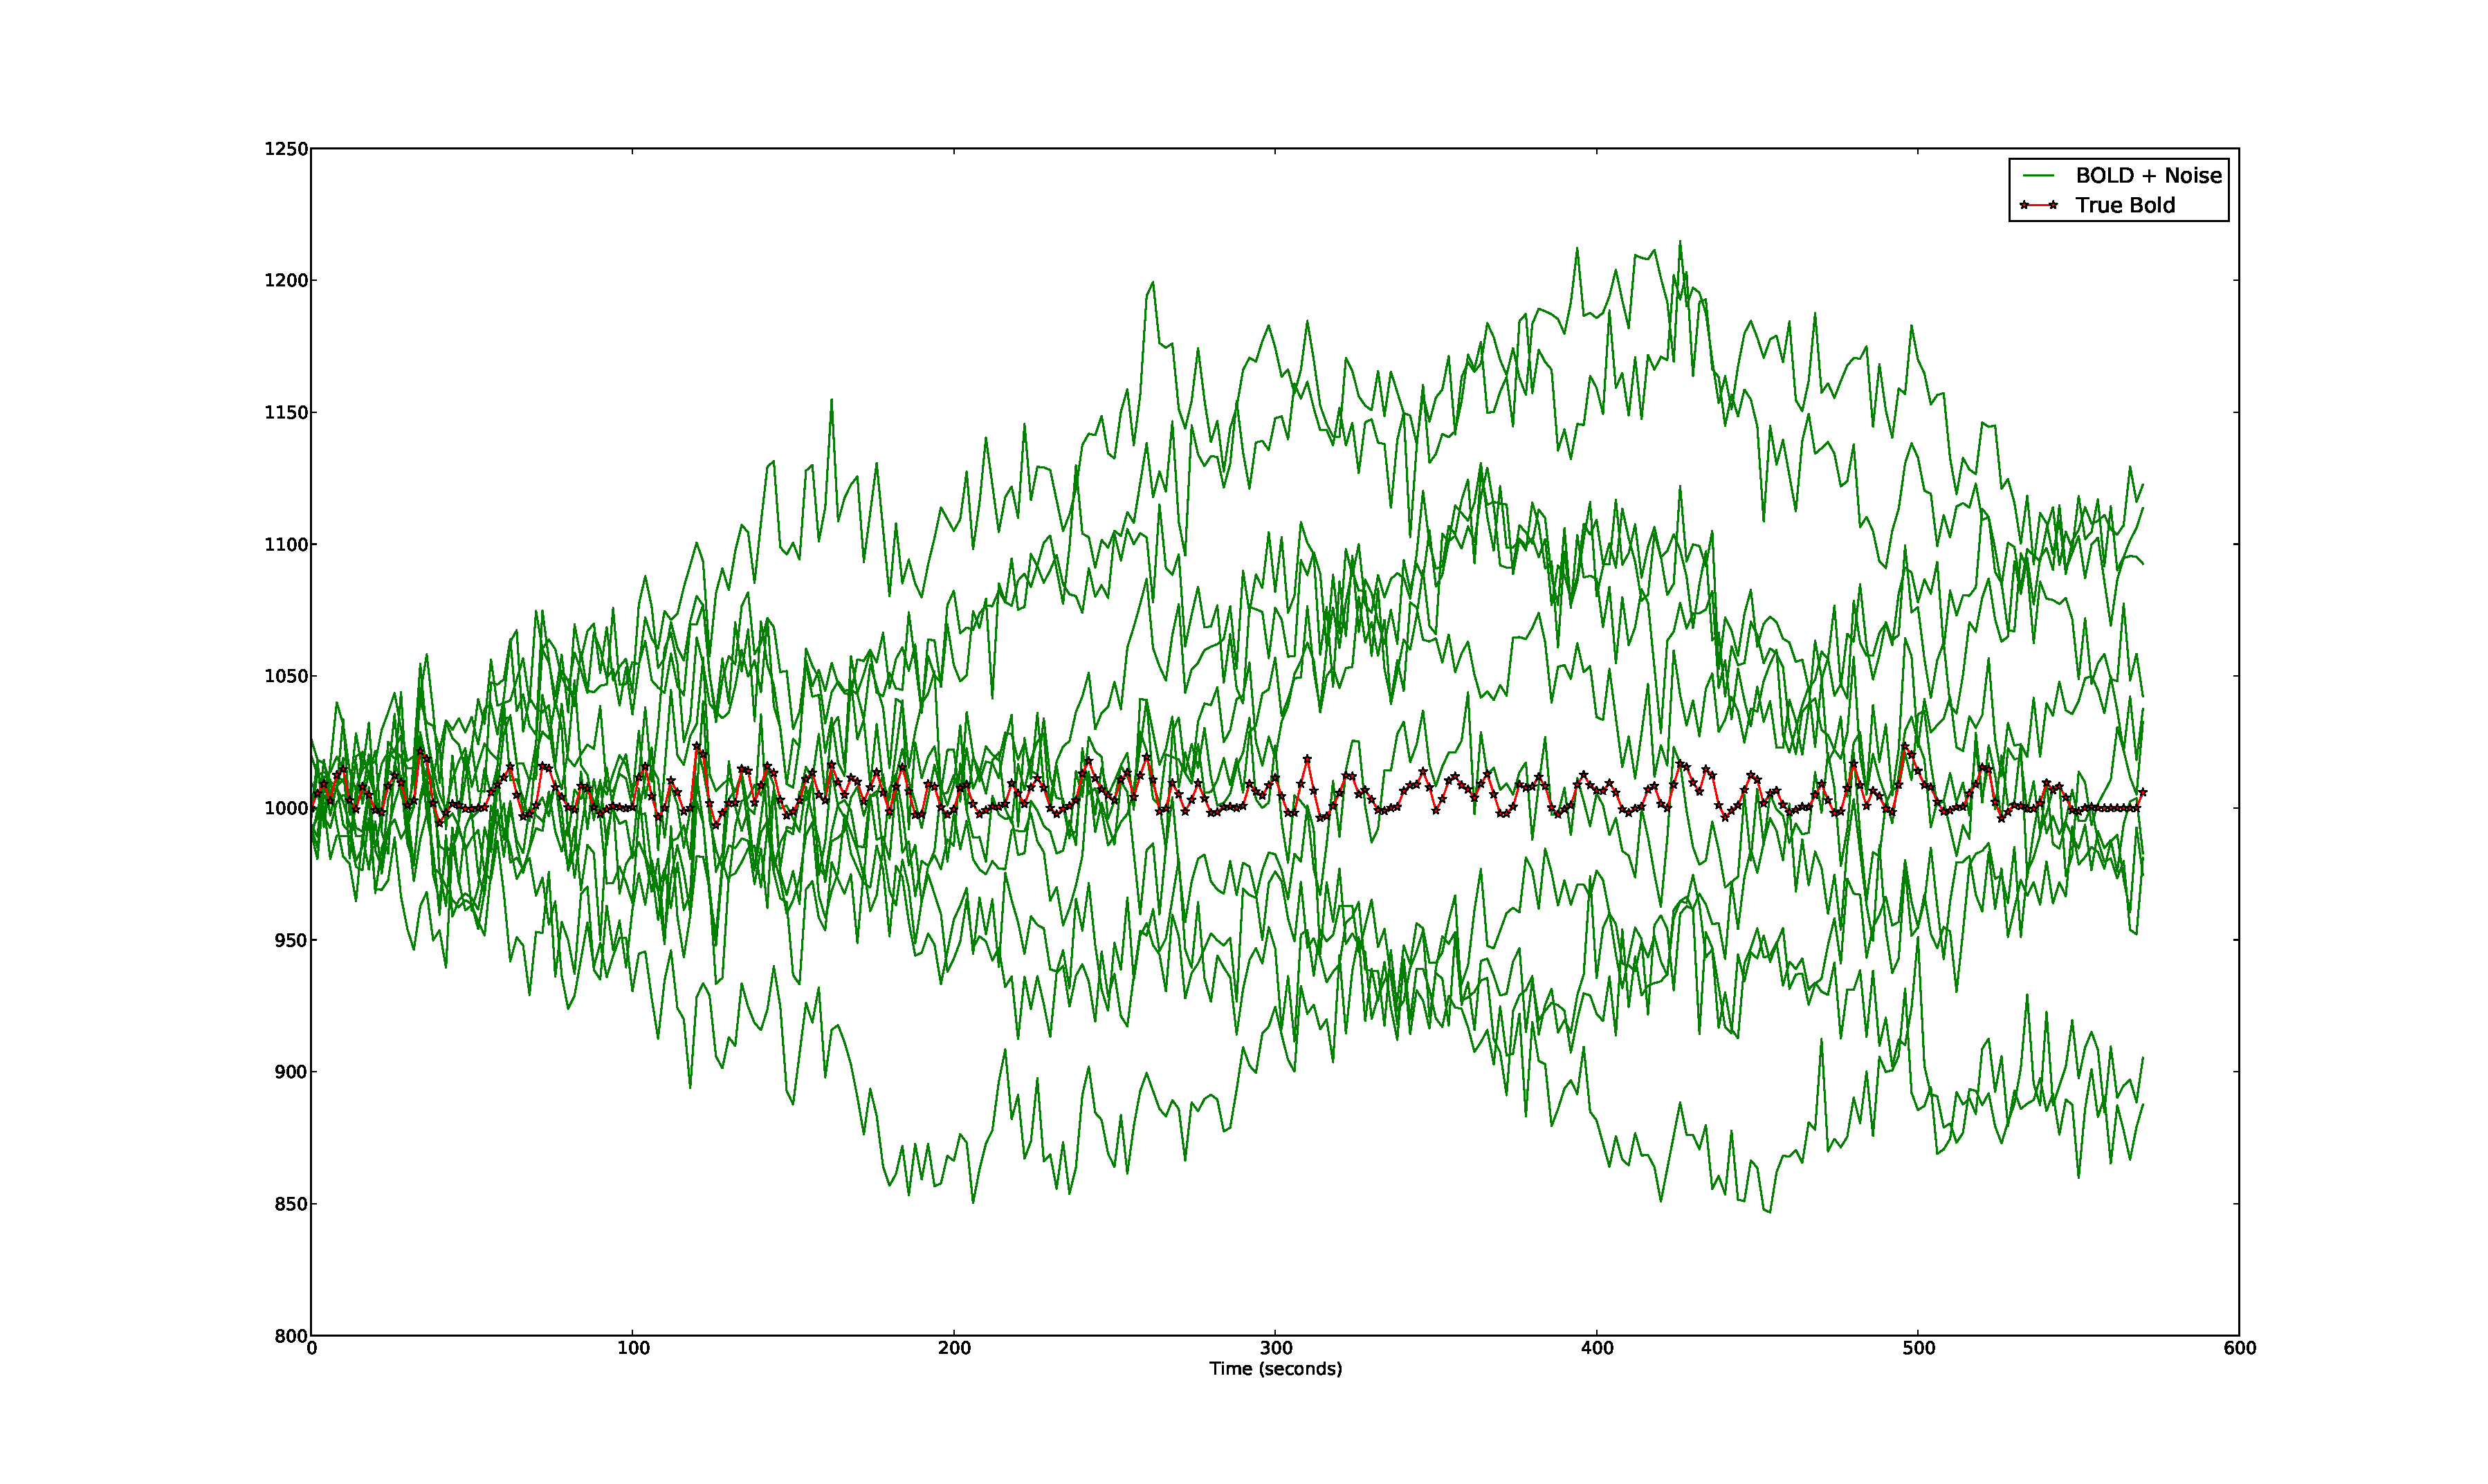
\includegraphics[clip=true,trim=6cm 2cm 5cm 3.5cm,width=15cm]{images/realization_highnoise}
%\caption{Test Signals with high noise ($\sigma_x = 0.01, \sigma_y=0.005$) compared to the clean signal.}
%\label{fig:HighNoiseRealization}
%\end{figure}

\begin{figure}
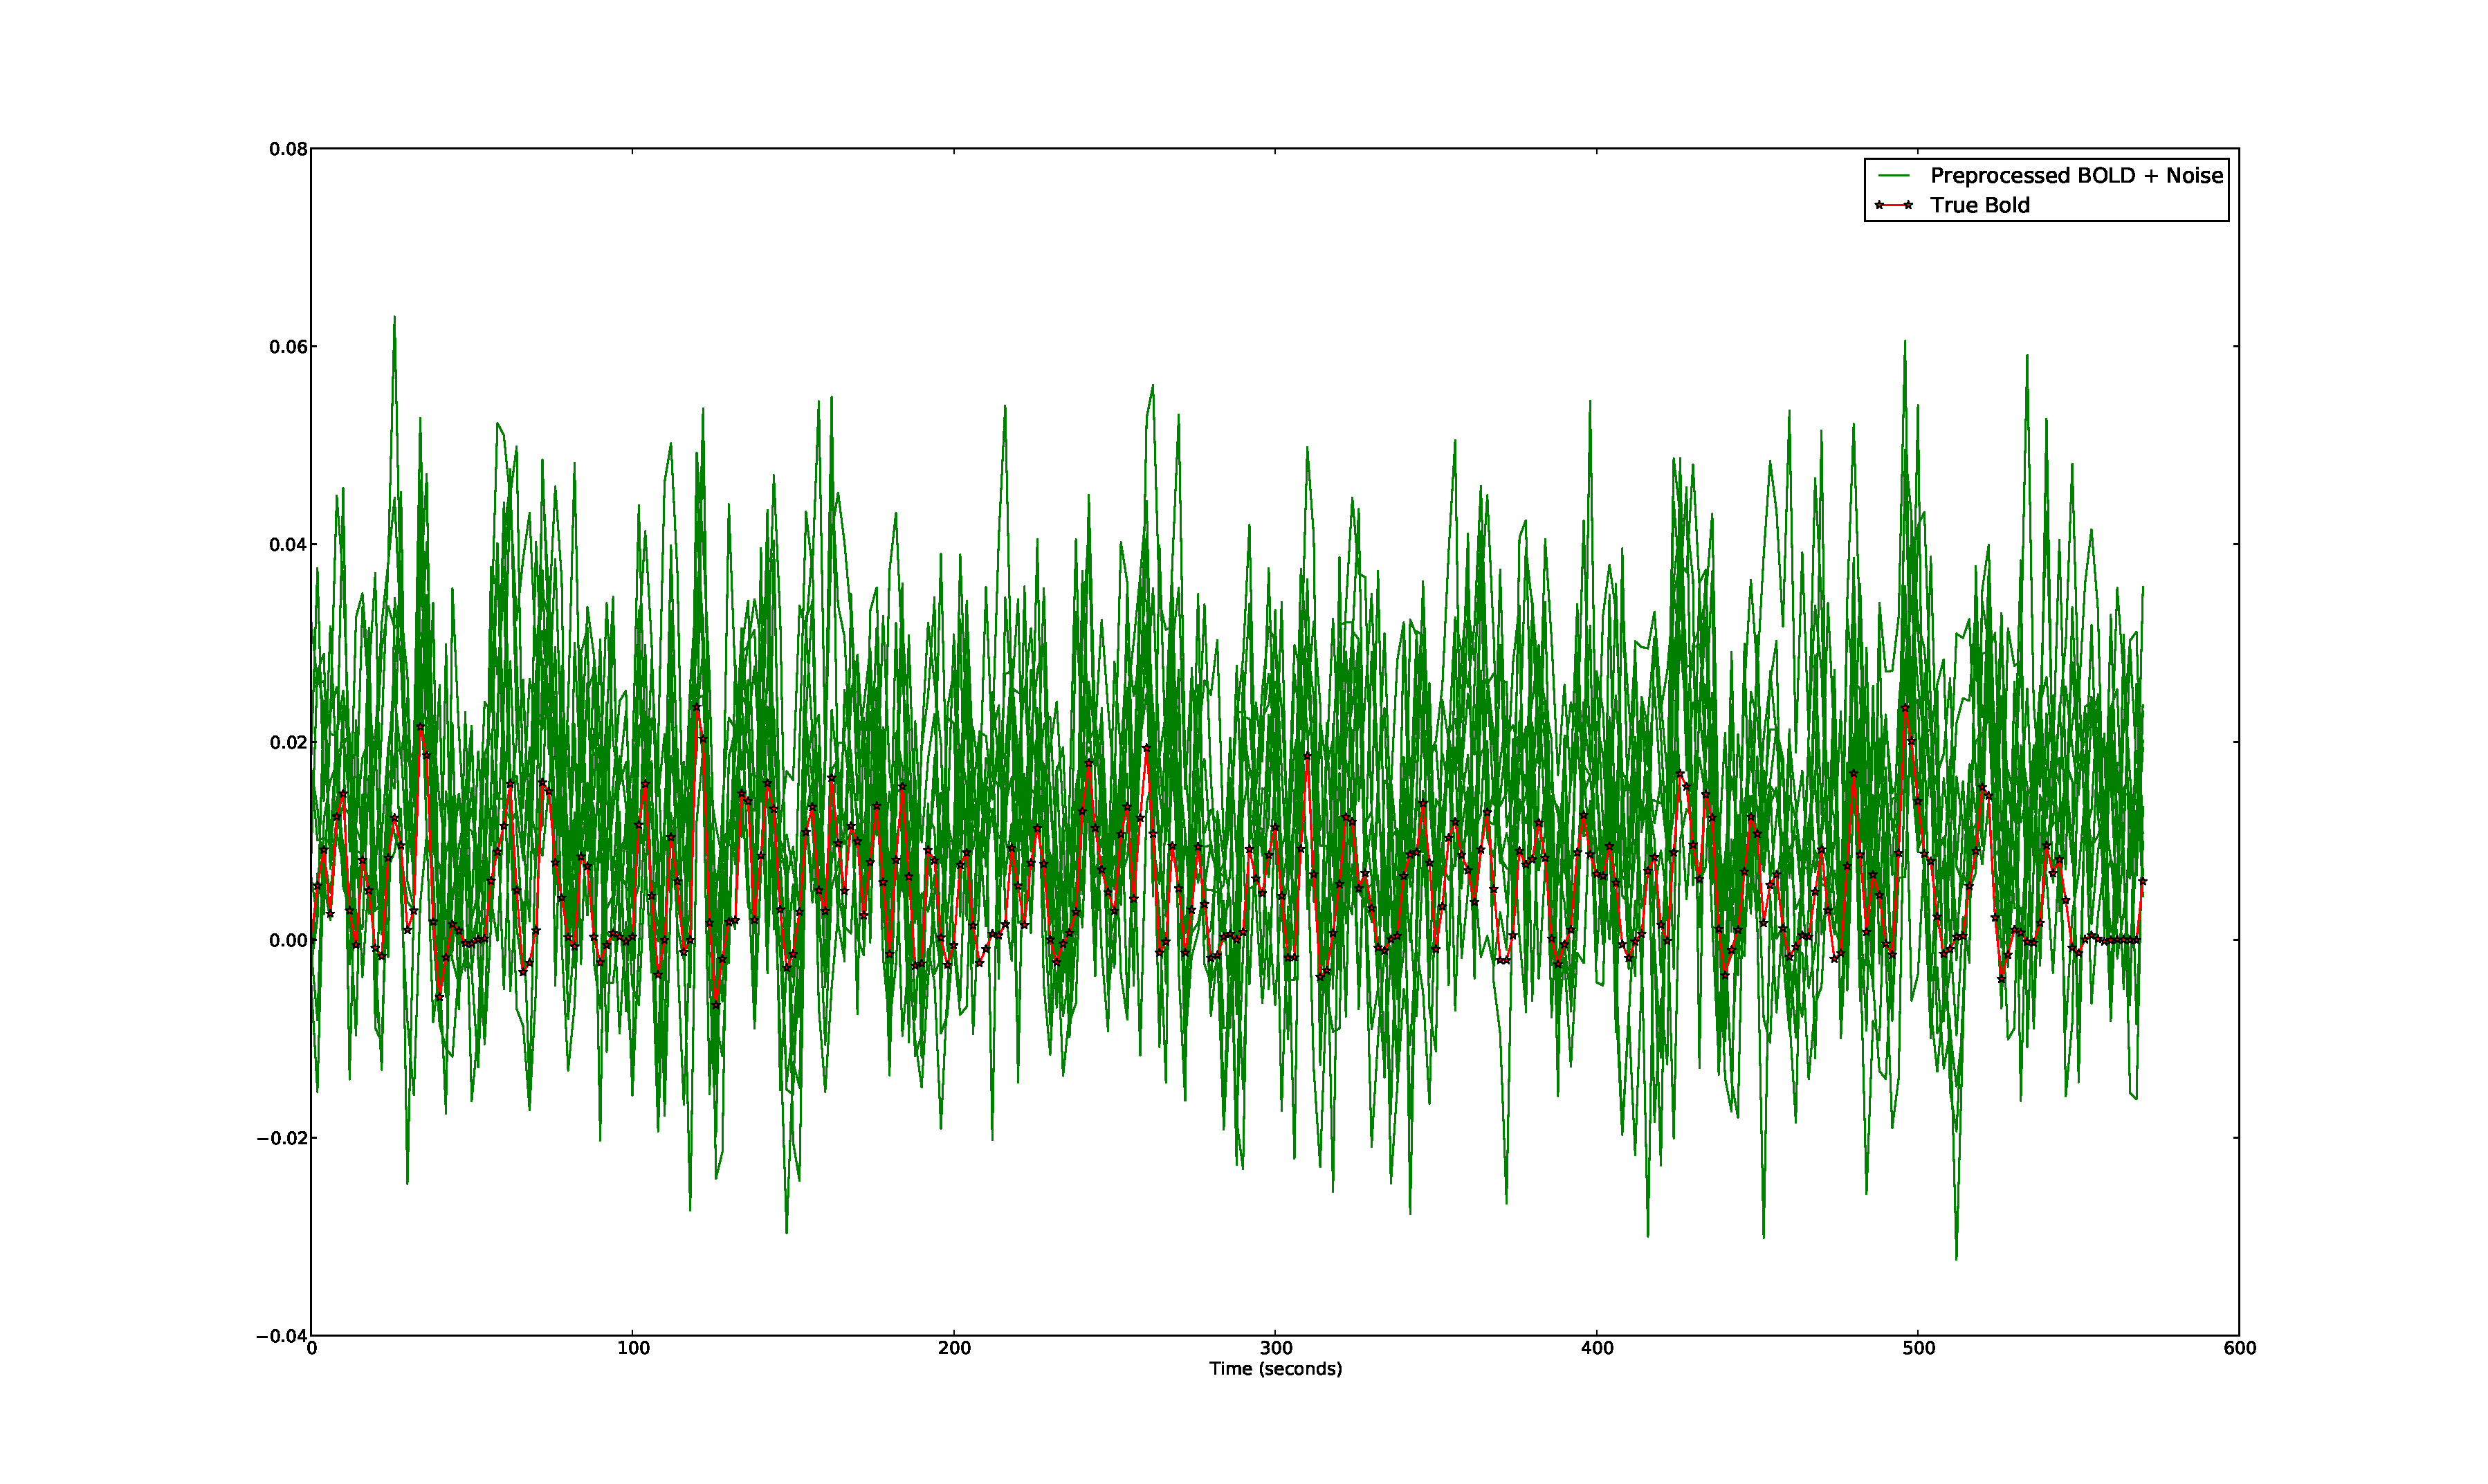
\includegraphics[clip=true,trim=6cm 2cm 5cm 3.5cm,width=15cm]{images/preprocessed_highnoise}
\caption[Preprocessed Signal with High Noise/Drift]
{Results of preprocessing compared to the true signal.  
 Knots of spline placed every 20 measurements. ($\sigma_x = 0.005$, $\sigma_y = 0.01$)}
\label{fig:PreprocessedHighNoise}
\end{figure}

\begin{figure}
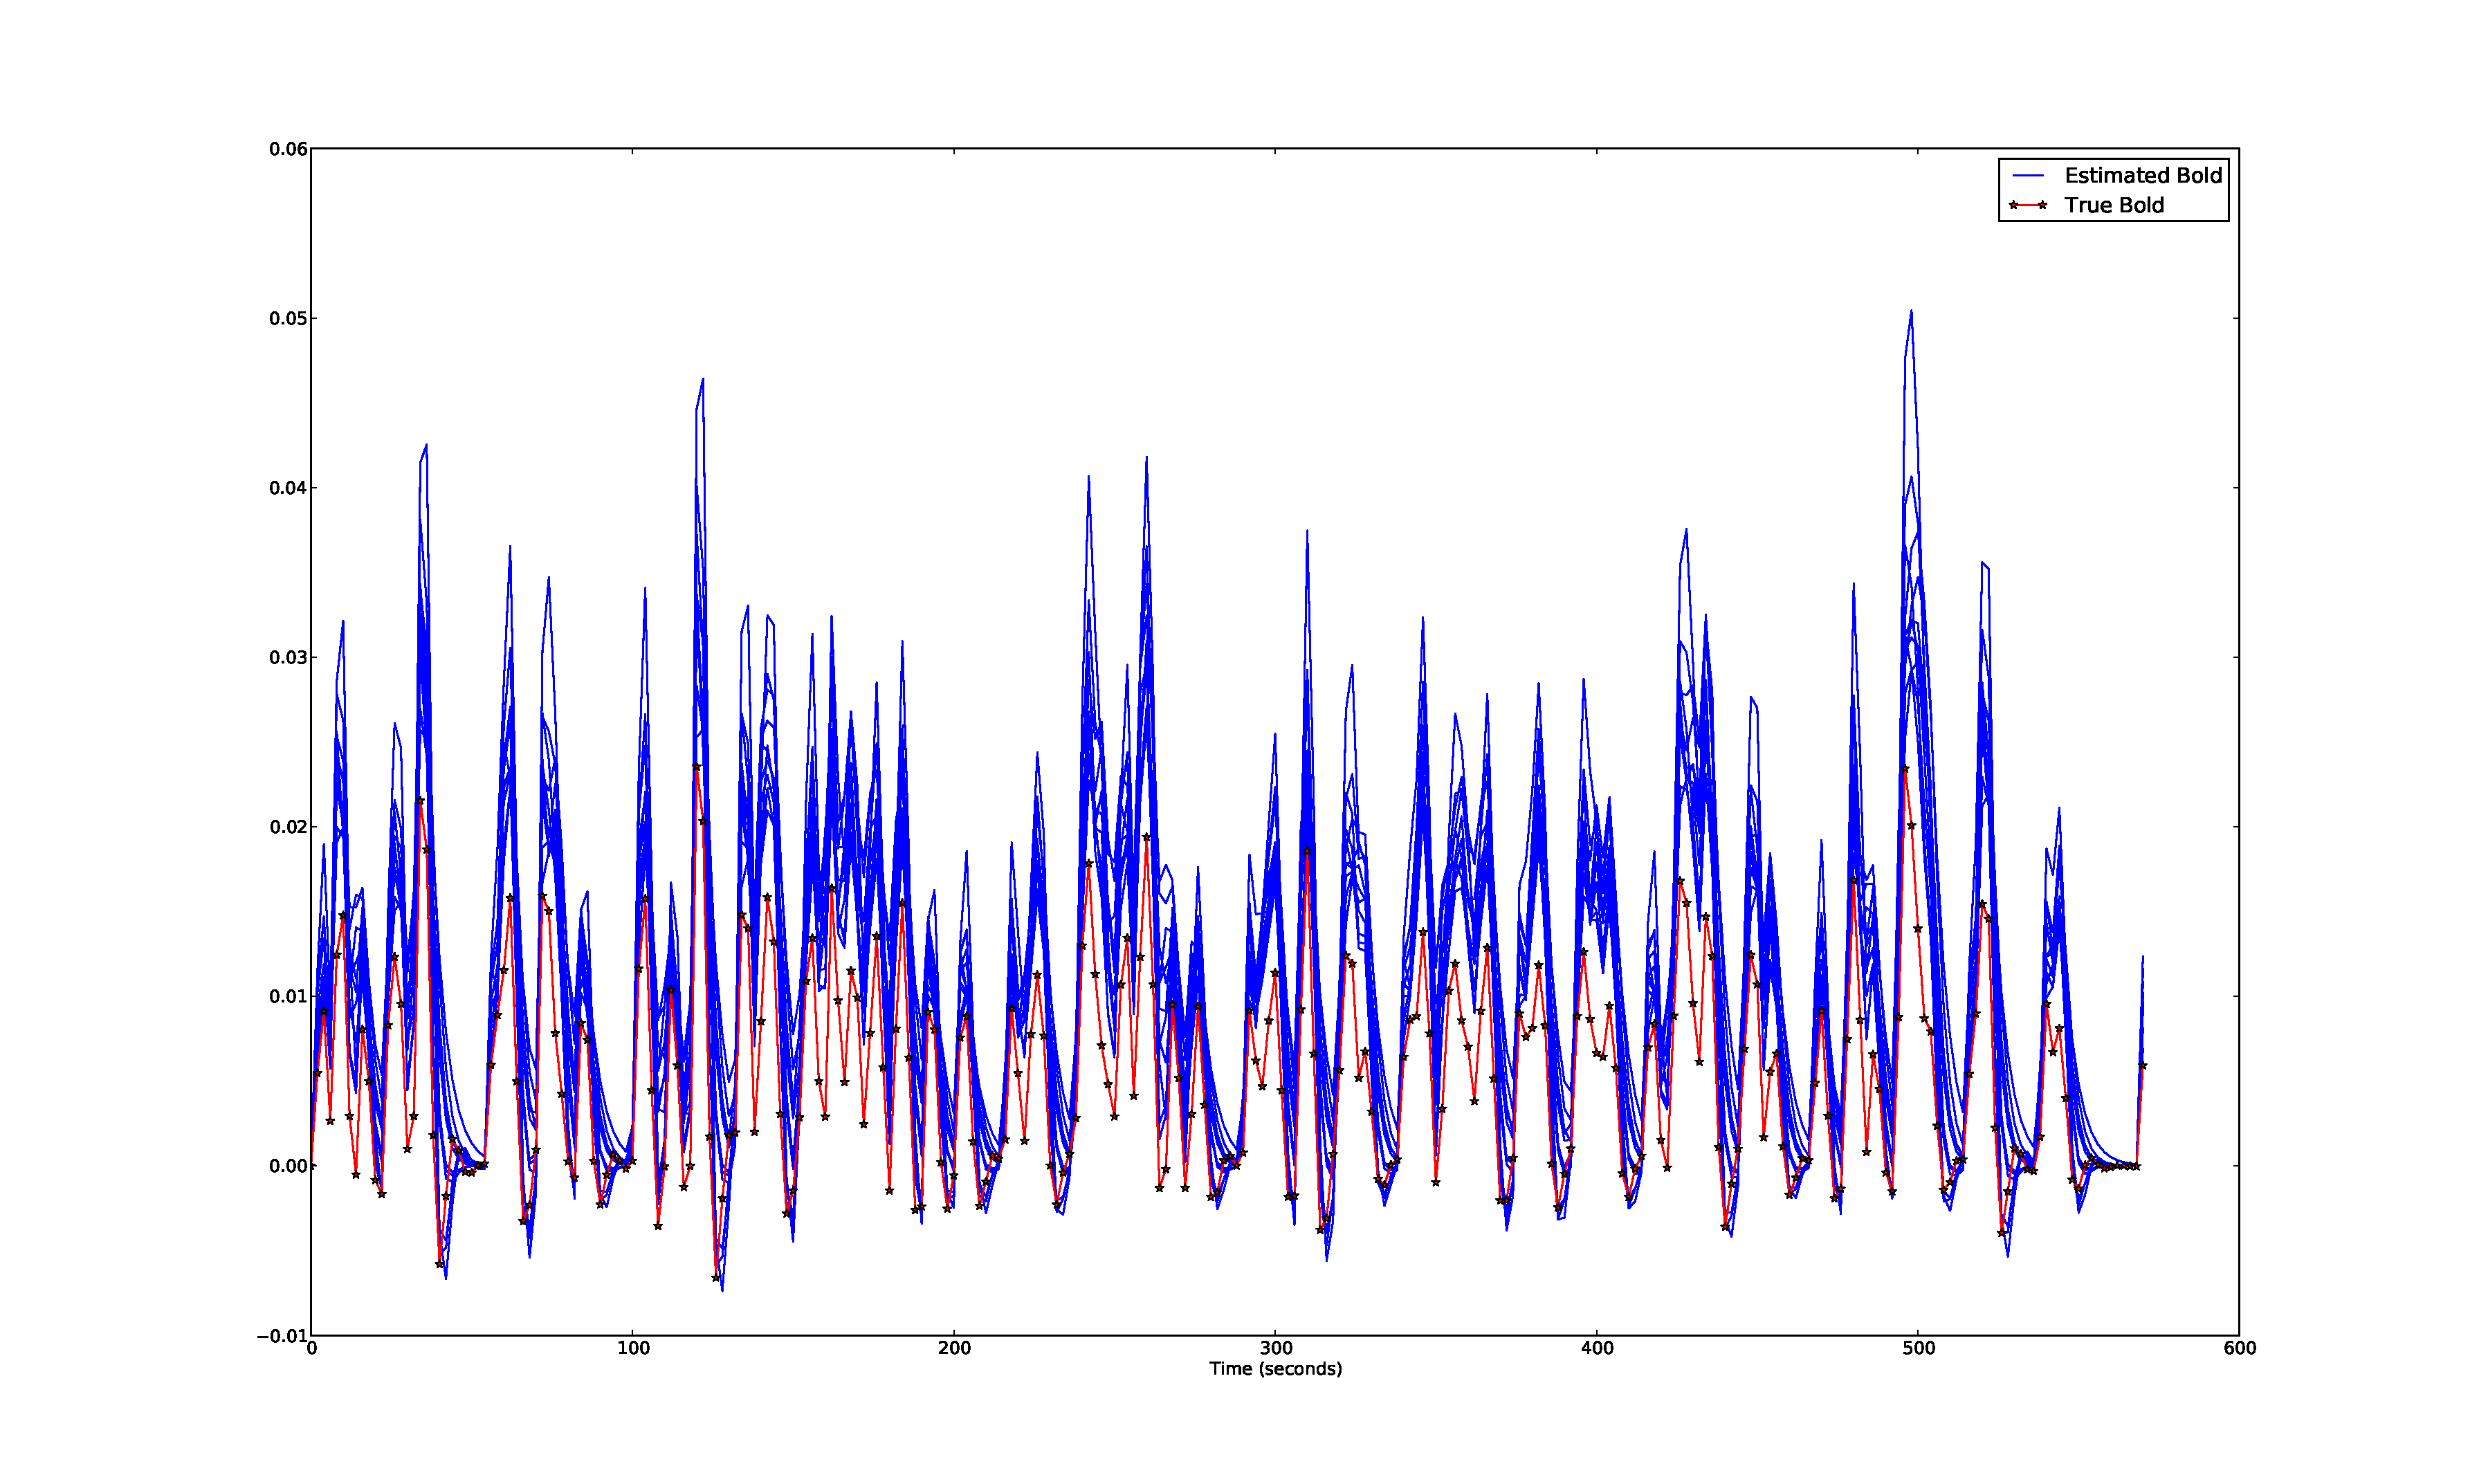
\includegraphics[clip=true,trim=6cm 2cm 5cm 3.5cm,width=15cm]{images/comparison_highnoise}
\caption[Results with High Noise/Drift]
{Results of the particles filter with preprocessed signals from \autoref{fig:PreprocessedHighNoise}
as input.}
\label{fig:FitComparisonHighNoise}
\end{figure}

\begin{figure}
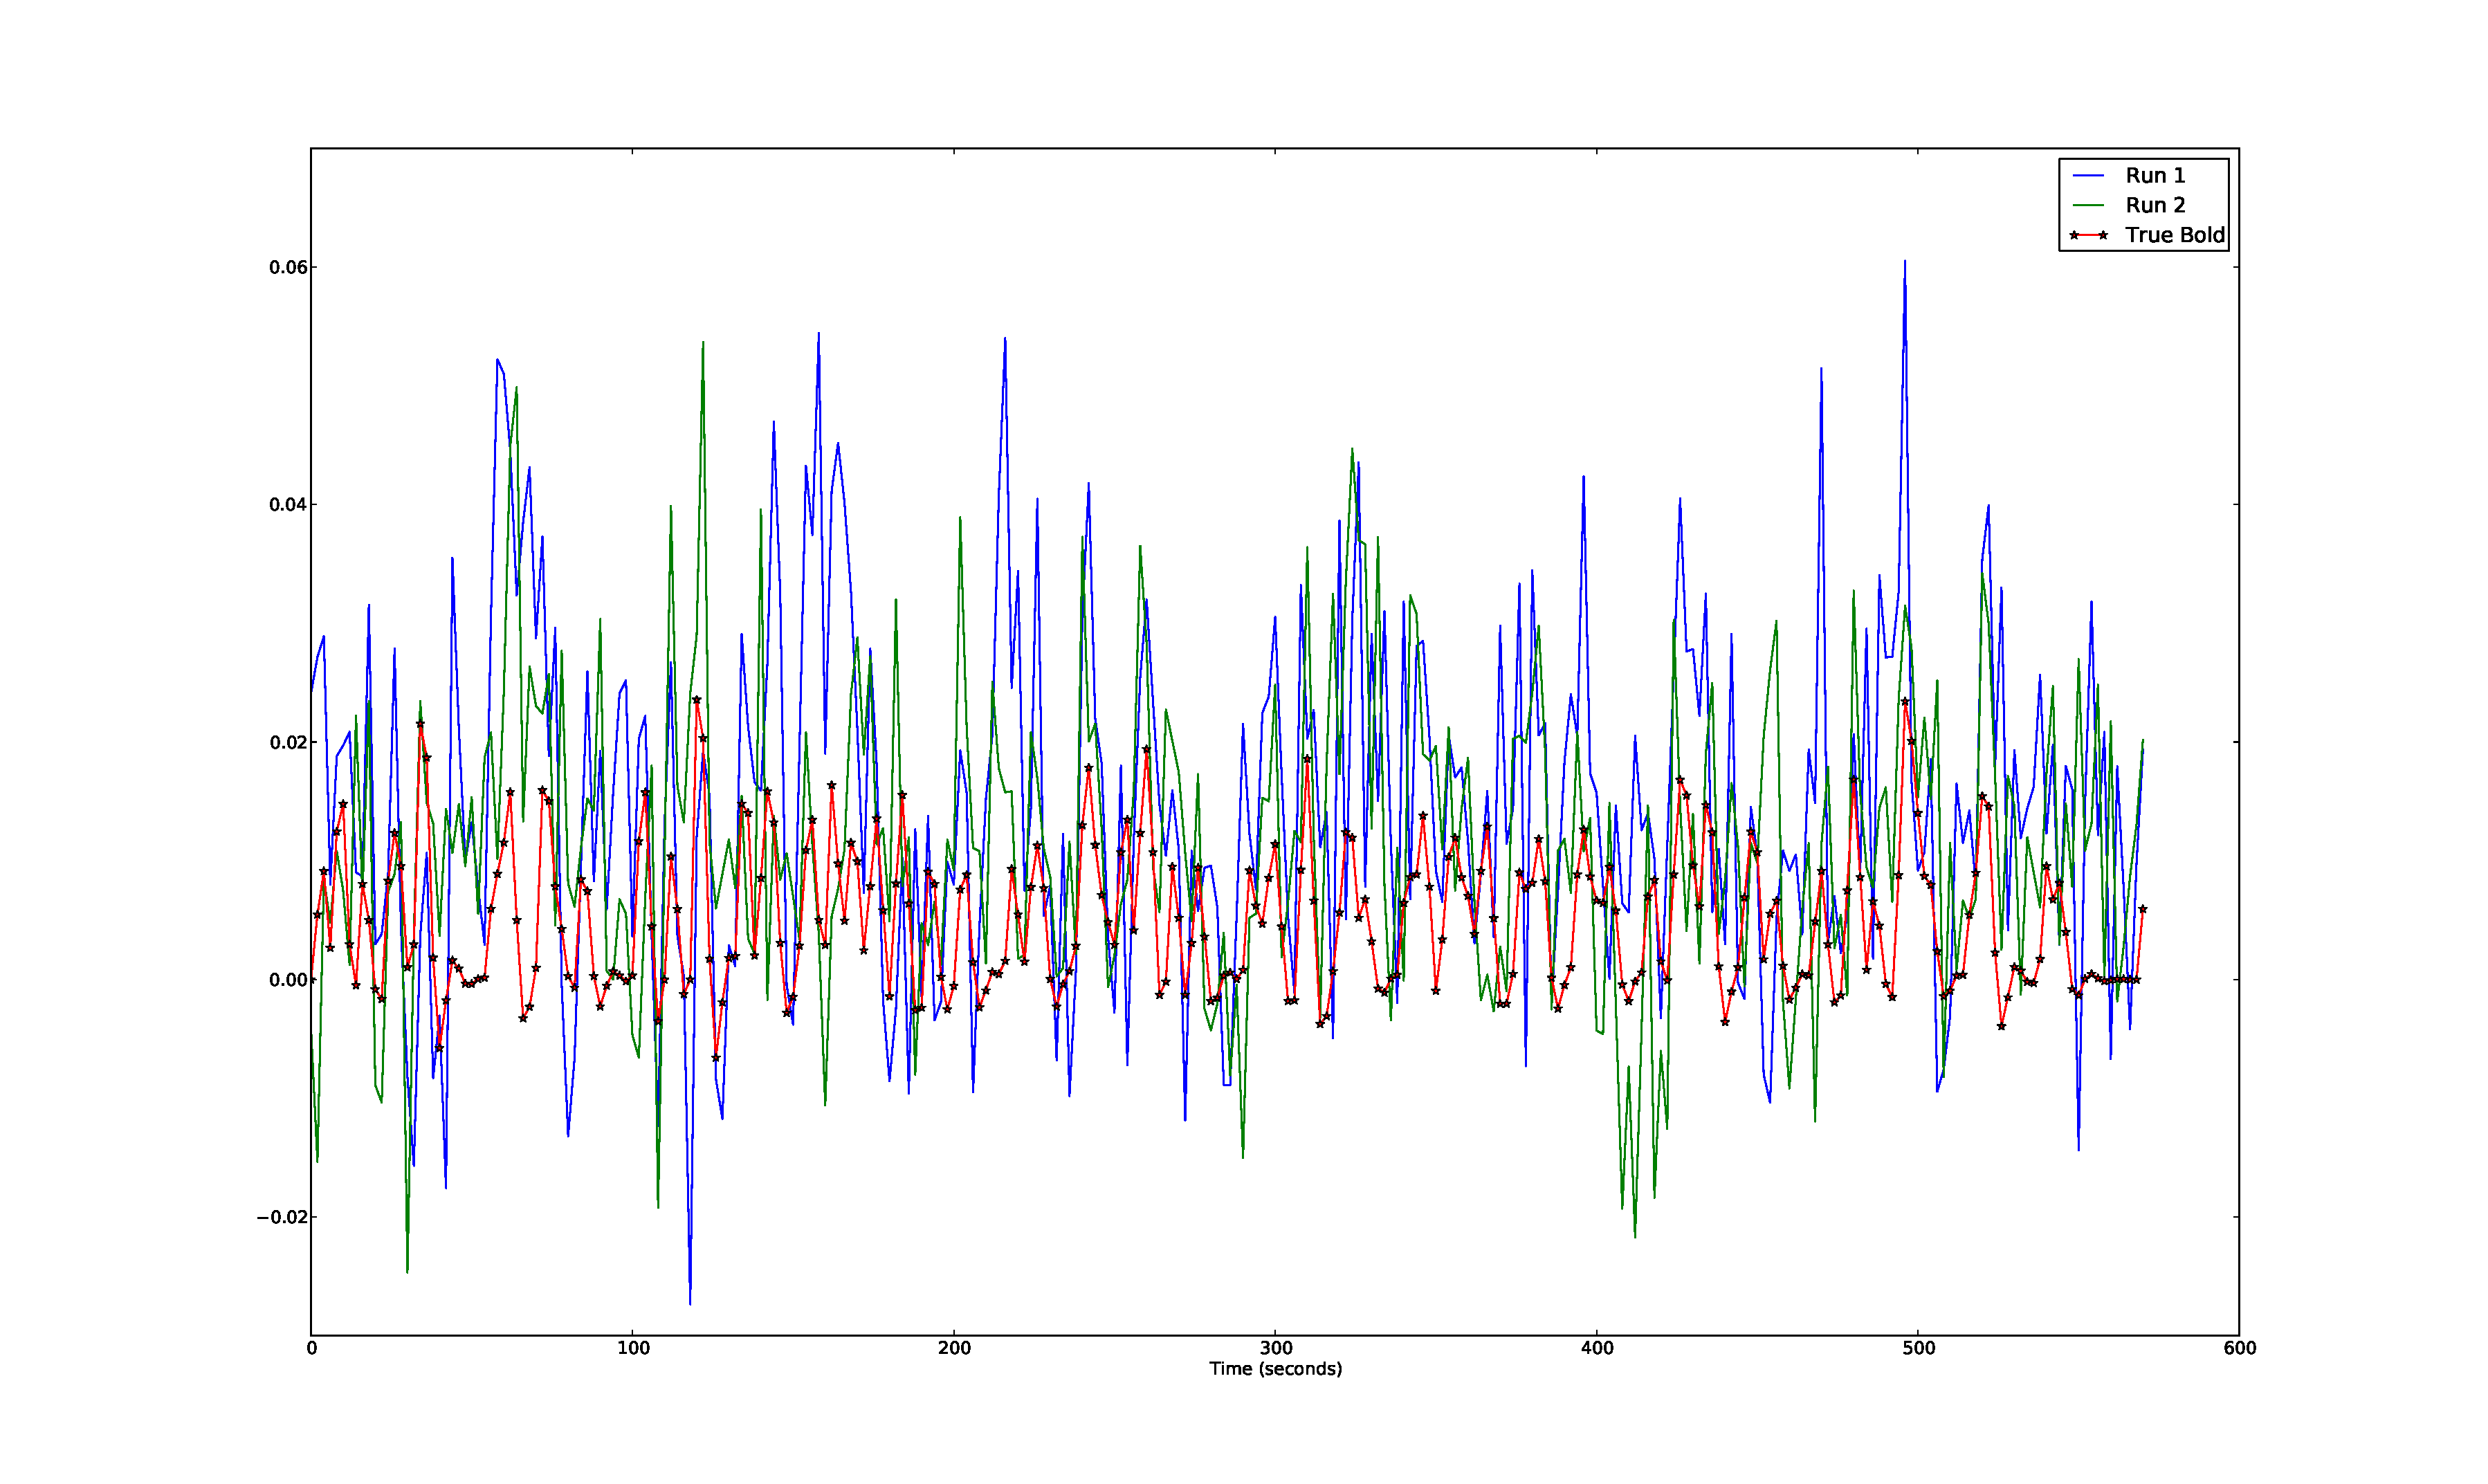
\includegraphics[clip=true,trim=6cm 2cm 5cm 3.5cm,width=15cm]{images/highnoise_56_noise}
\caption{Two particular preprocessed noise realizations for the high noise case.}
\label{fig:NoiseComparisonJustTwo}
\end{figure}

\begin{figure}
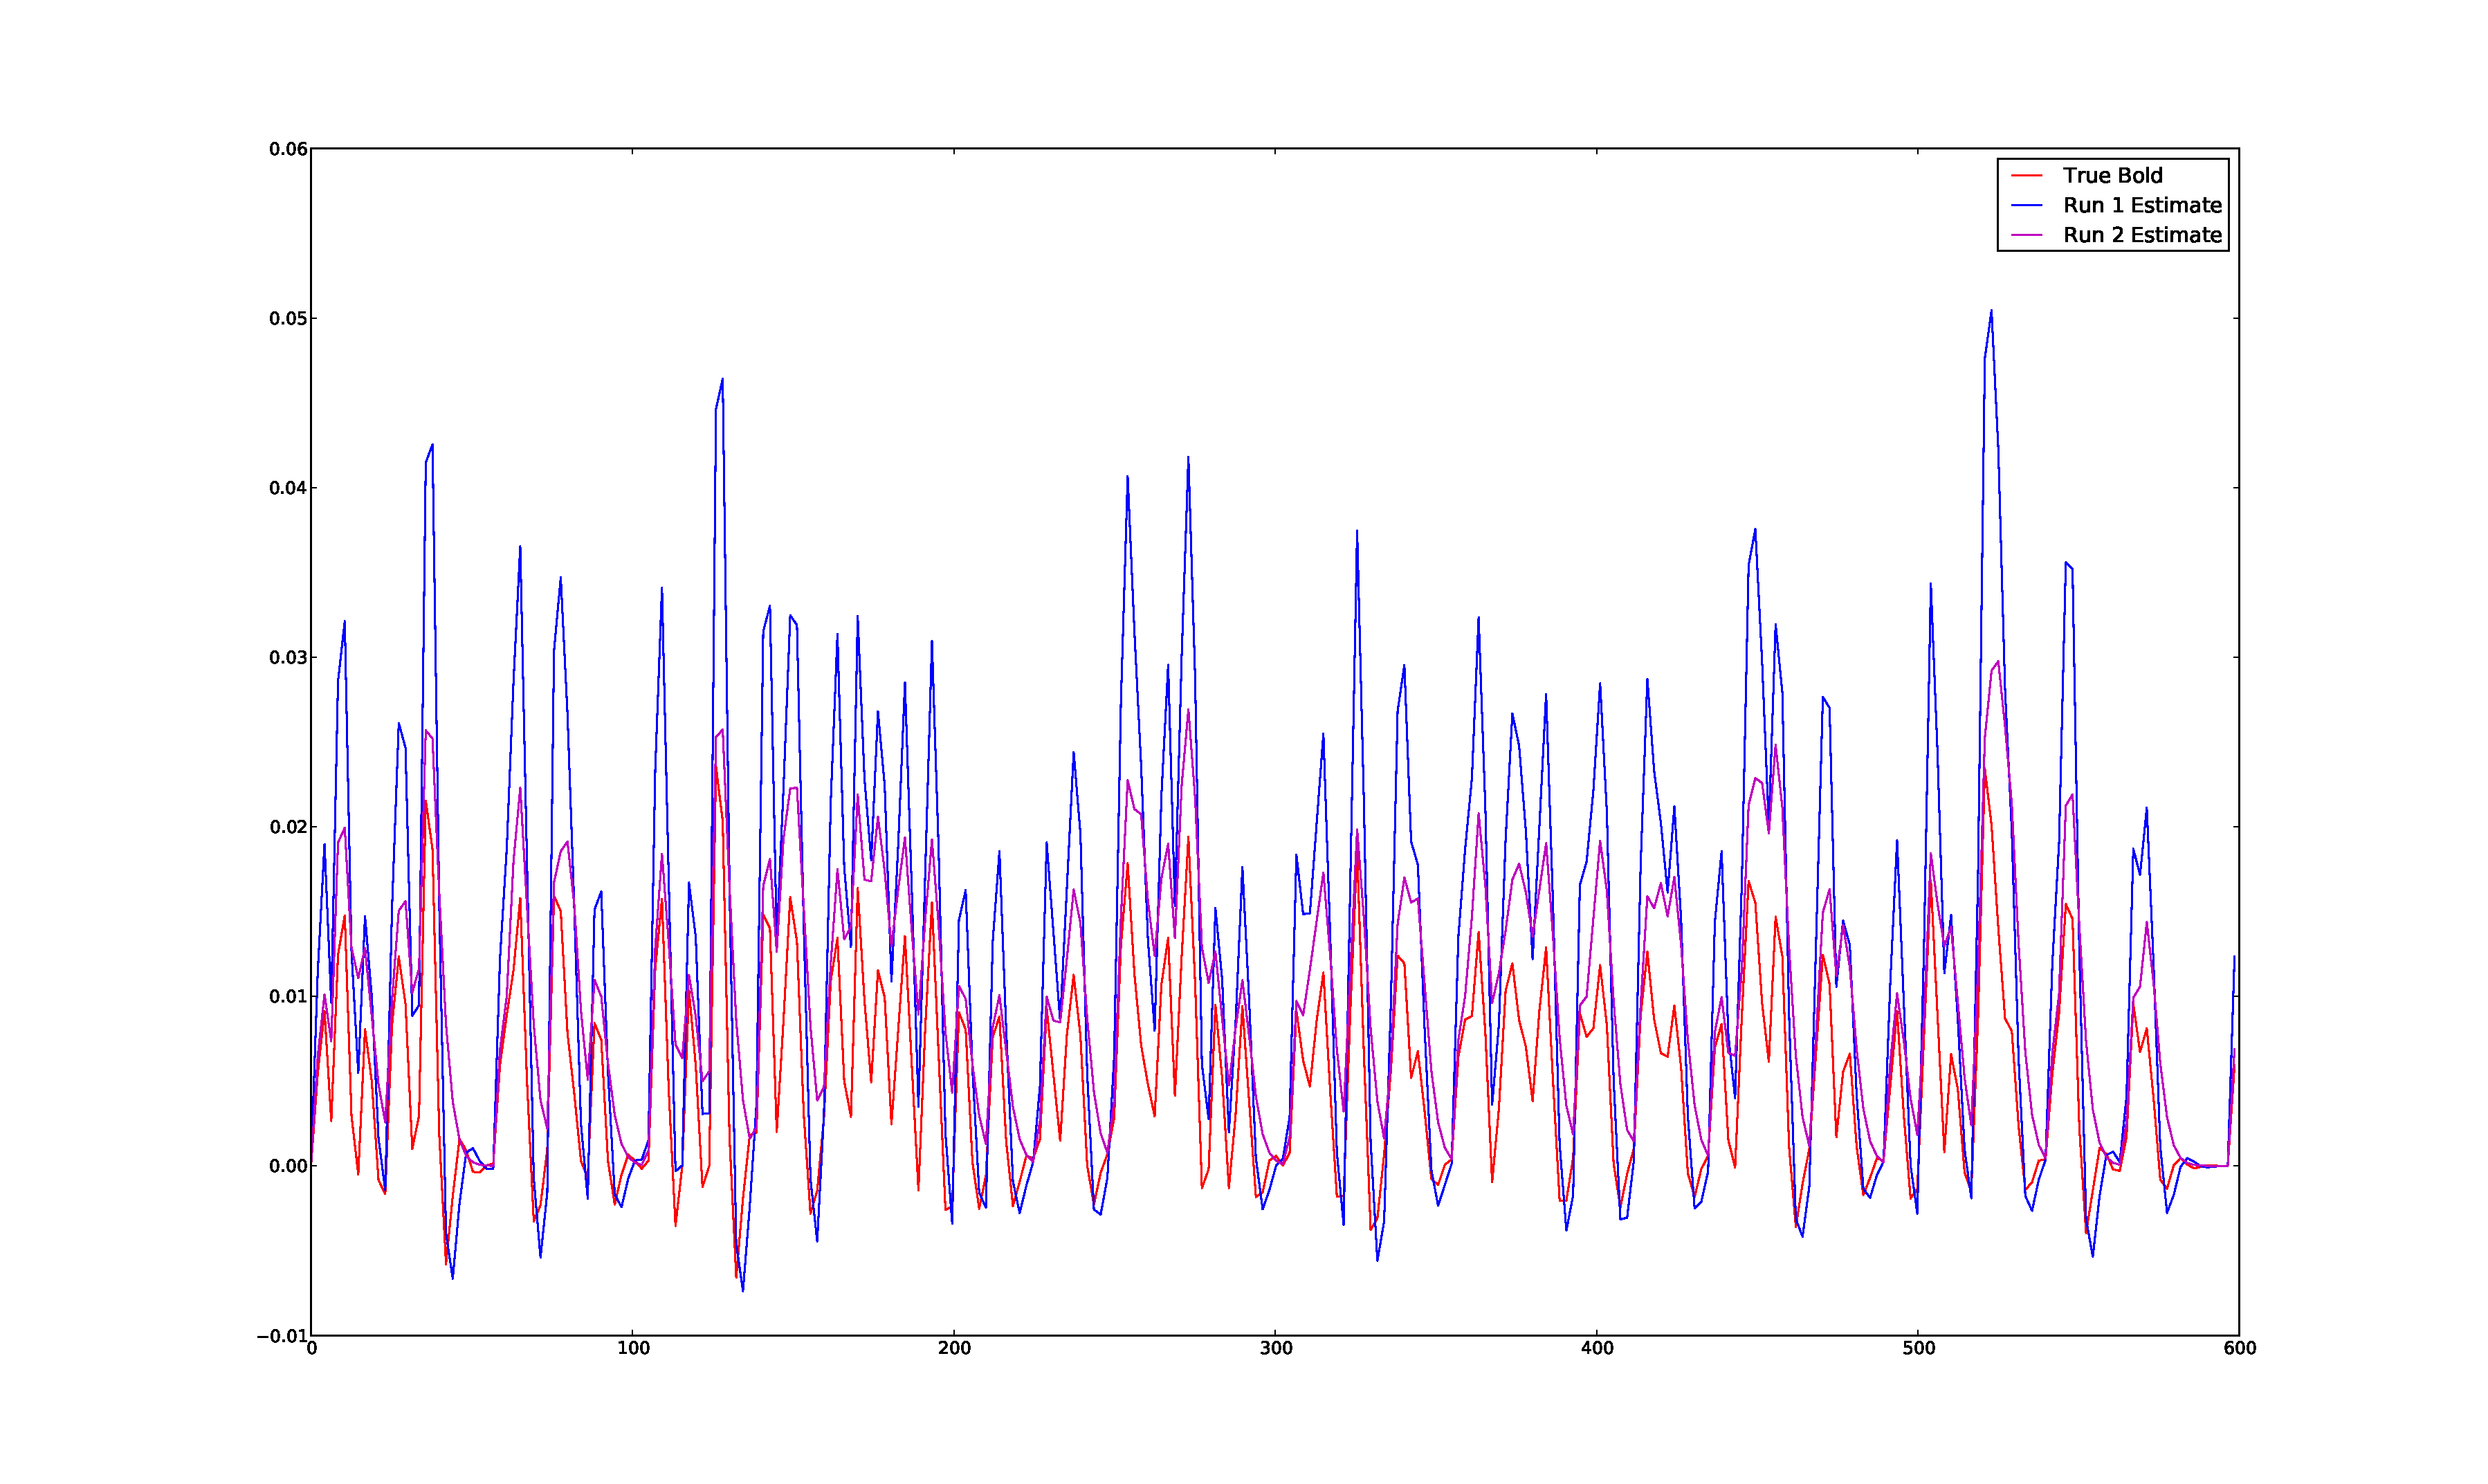
\includegraphics[clip=true,trim=6cm 2cm 5cm 3.5cm,width=15cm]{images/comparison_highnoise_just2}
\caption{The results for the noise realizations shown in \autoref{fig:NoiseComparisonJustTwo}.}
\label{fig:FitComparisonHighNoiseJust2}
\end{figure}

For the high noise simulation, the exact same procedure was followed as in \autoref{sec:SimLowNoise}
except that $\sigma_y$ and $\sigma_x$ were set to $0.01$ and $0.005$,
respectively. This is an order of magnitude higher than the previous tests, and indeed the
noise appears to dominate the output, as \autoref{fig:PreprocessedHighNoise} shows.
The results of the particle filter
for each of the eleven runs are shown in \autoref{fig:FitComparisonHighNoise}.
The noise and preprocessing again led the estimates
to higher peak activation levels, and the subtleties of different time constants
were lost in the noise.

\begin{table}[t]
\centering
\begin{tabular}{|c | c | c | c | c | c | c | c | c | c |}
\hline
$\tau_0$ & $\alpha$ & $E_0$    & $V_0$    & $\tau_s$ & $\tau_f$ & $\epsilon$  & $ \sum \tau $ & \acs{RMSR} & \acs{RMSE} \\
\hline
\rowcolor[gray]{.8}
1.45 & 0.3 & 0.47 & 0.044 & 1.94 & 1.99 & 1.8  & 5.38 &  & \\
\hline
\hline
1.1900 & 0.2349 & 0.4223 & 0.128  & 1.0147 & 2.4779 & 1.1168 & 4.6826 &0.01406 & 0.00859\\
0.9721 & 0.2190 & 0.3051 & 0.061  & 0.5780 & 1.9960 & 3.4613 & 3.5461 &0.01373 & 0.00735\\
1.5795 & 0.1415 & 0.3380 & 0.1089 & 0.5843 & 2.1247 & 1.7834 & 4.2885 &0.01275 & 0.00951\\
1.1094 & 0.2374 & 0.5349 & 0.0351 & 1.2186 & 3.0736 & 2.3504 & 5.4016 &0.01673 & 0.00479 \\
1.1071 & 0.2753 & 0.3365 & 0.0316 & 1.5057 & 2.6518 & 4.1910 & 5.2646 &0.01370 & 0.00475\\
0.5803 & 0.4793 & 0.4135 & 0.1189 & 0.9756 & 3.6902 & 1.0008 & 5.2461 &0.01150 & 0.00672\\
\rowcolor[rgb]{.9,.5,.5}
1.2952 & 0.2596 & 0.2756 & 0.2595 & 1.7026 & 2.8458 & 0.6617 & 5.8436 &0.01555 & 0.01039\\
\rowcolor[rgb]{.5,.5,.9}
1.5185 & 0.2199 & 0.2835 & 0.0742 & 0.8882 & 3.0771 & 1.7393 & 5.4838 &0.01205 & 0.00655\\
0.6874 & 0.3283 & 0.3979 & 0.1561 & 1.0778 & 3.1158 & 0.6643 & 4.8810 &0.01510 & 0.0057 \\
1.0170 & 0.285  & 0.3474 & 0.0567 & 1.5877 & 2.6516 & 2.2852 & 5.2563 &0.01249 & 0.00582\\
0.9925 & 0.298  & 0.3221 & 0.2094 & 0.4276 & 2.2108 & 1.0167 & 3.6308 &0.01217 & 0.00916\\
\hline
1.0954 & 0.2708 & 0.3615 & 0.1126 & 1.0510 & 2.7196 & 1.8428 & 4.8659 &0.01362 & 0.00721\\
\hline
\end{tabular}
\caption[Estimated Parameters on 11 different runs with high noise.]
{Estimated Parameters on 11 different runs with high noise. First row contains the true parameters,
last row contains the mean.
The red row is Run 1 and the blue row is Run 2 from  \autoref{fig:NoiseComparisonJustTwo}
and \autoref{fig:FitComparisonHighNoiseJust2}, respectively.}
\label{tab:HighNoiseResults}
\end{table}

\autoref{fig:NoiseComparisonJustTwo} shows two runs in more detail; these
results show that more drift was present that 20 measurements per knot 
could fit. Insufficient flexibility of the spline explains
the prolonged increase at 170 seconds in Run 1; although such areas
permeate the preprocessed signals.
Interestingly, Run 1 and Run 2 emphasize
different aspects of the signal. Run 2 had a much better match to the
peaks, when compared to the true signal, yet Run 1 matched the post-stimulus
undershoot better.  \autoref{tab:HighNoiseResults} shows
the \ac{RMSE} for all eleven runs, and highlights the two runs analyzed
in \autoref{fig:ConvergenceRuns1} and \autoref{fig:ConvergenceRuns2}.

\begin{figure}[H]
\subfigure
{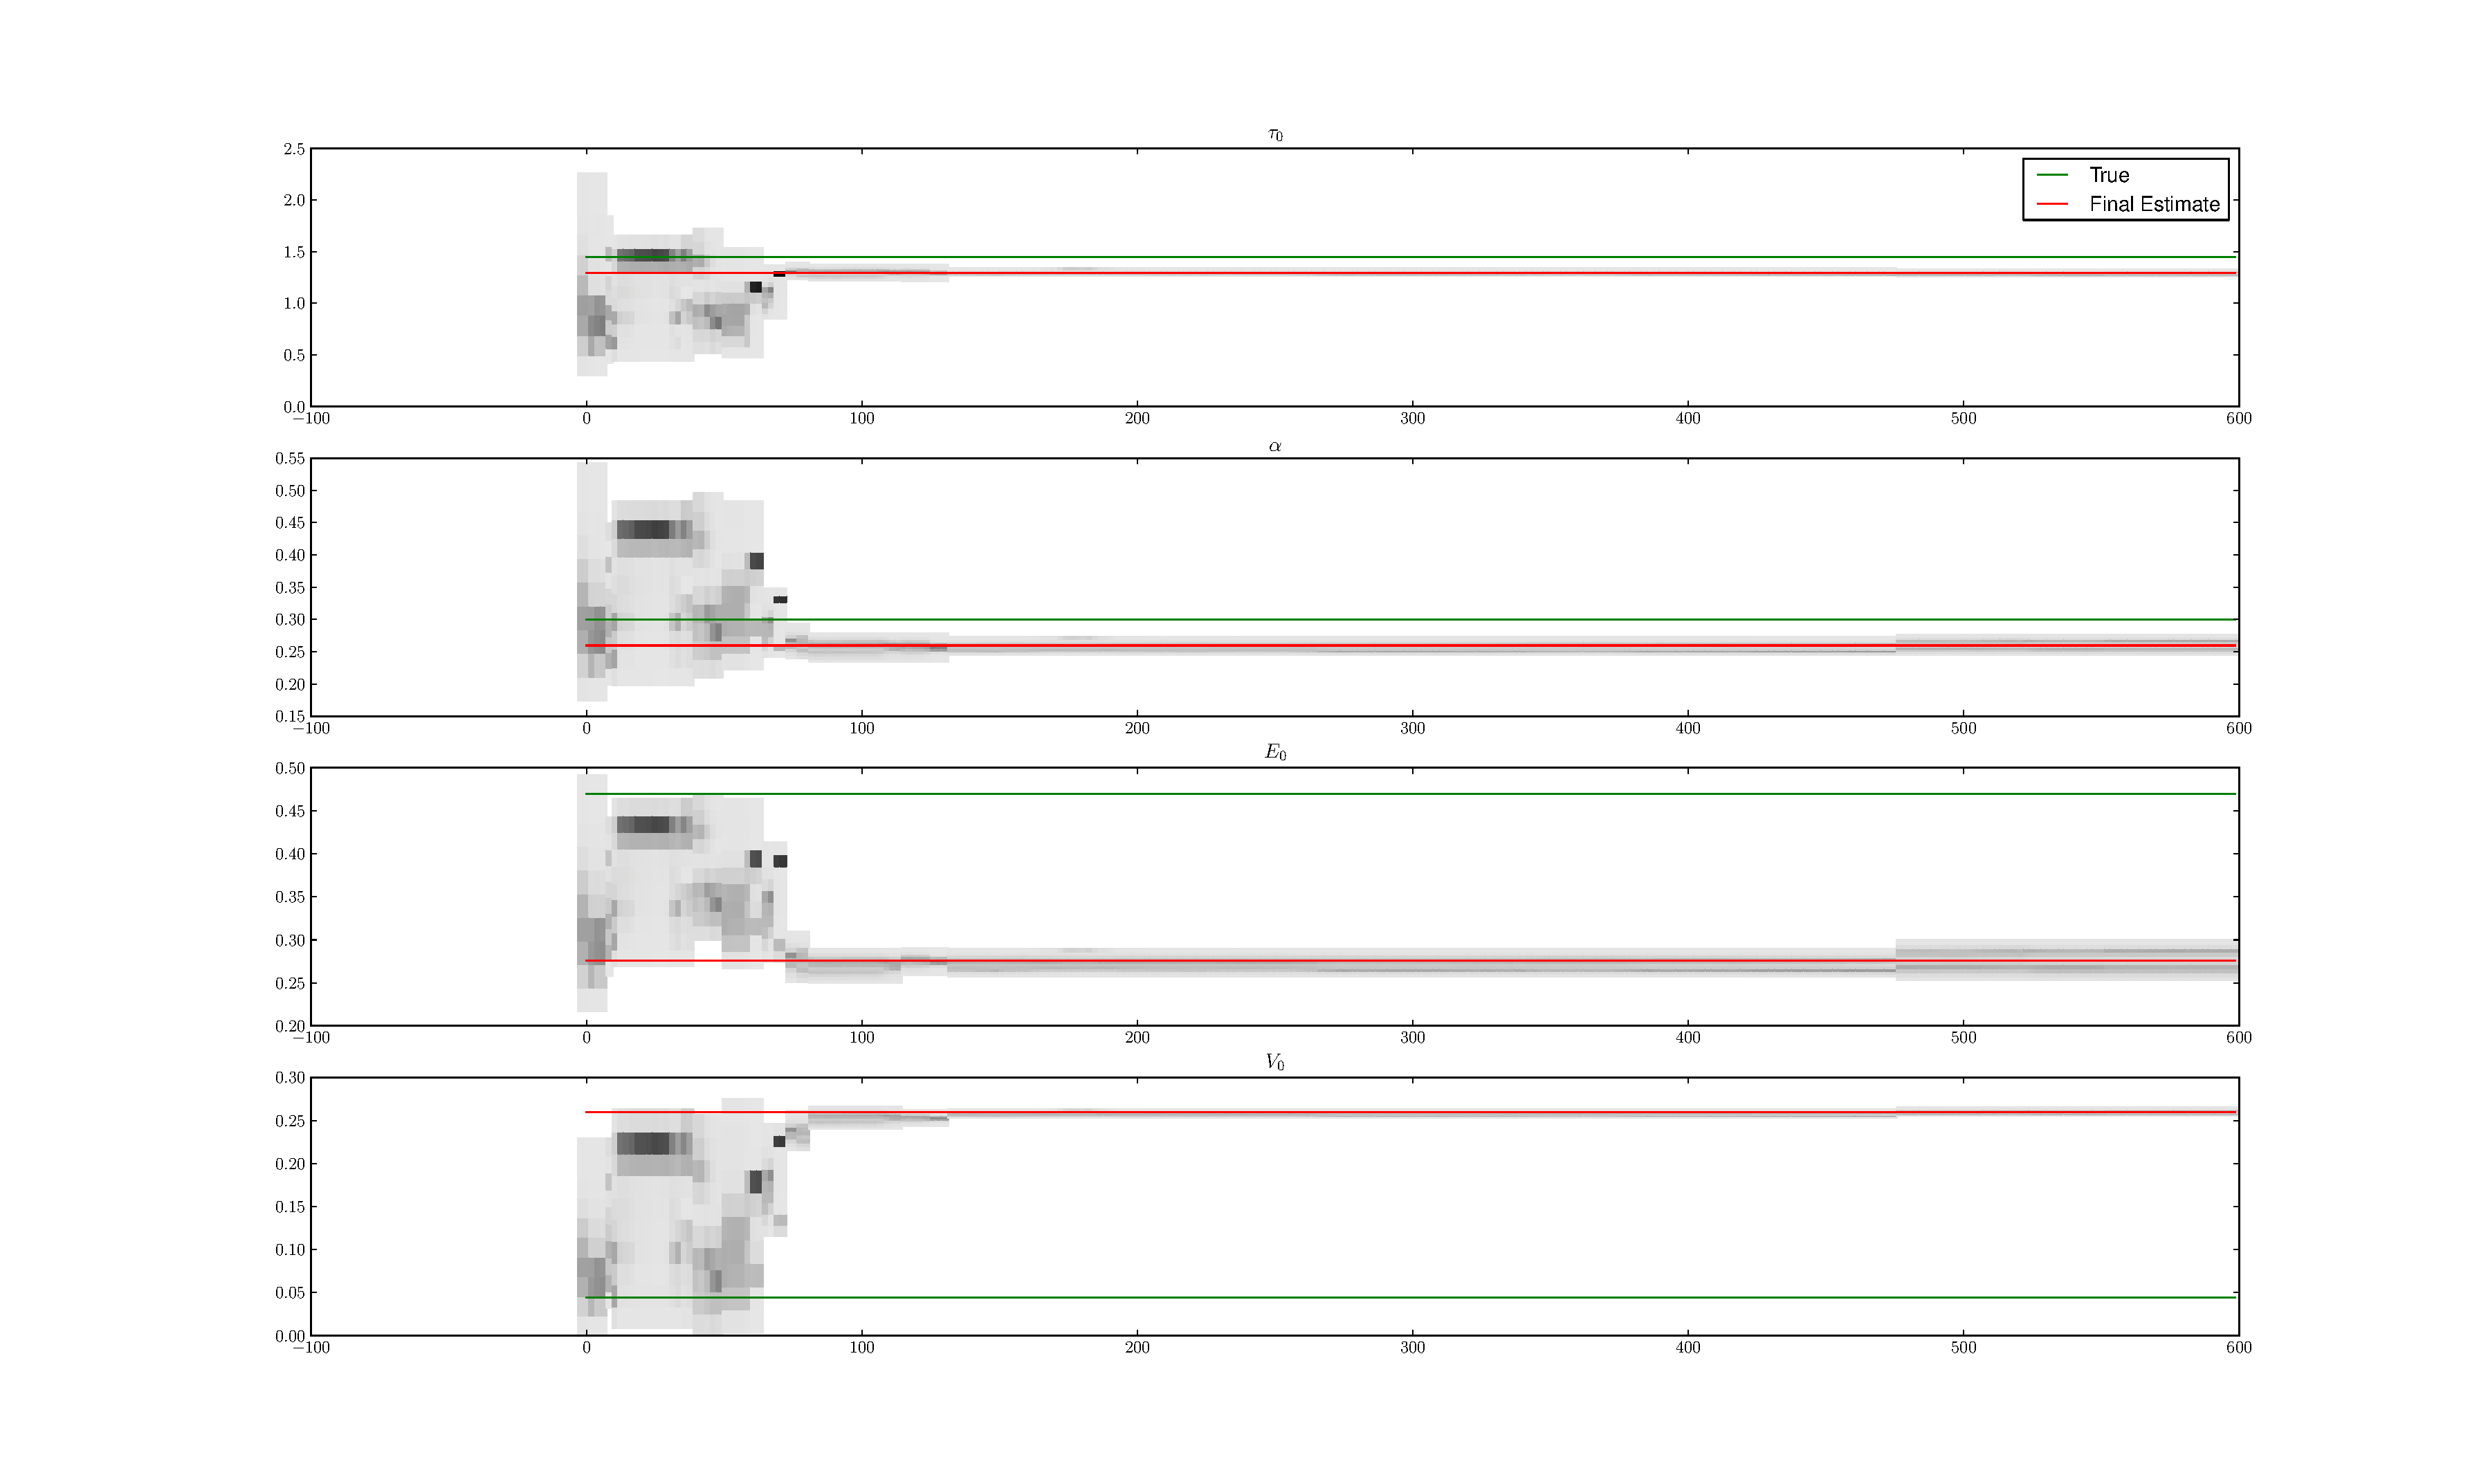
\includegraphics[clip=true,trim=6cm 2cm 6cm 3cm, width=\textwidth]{images/highnoise_run5_1}}
\subfigure
{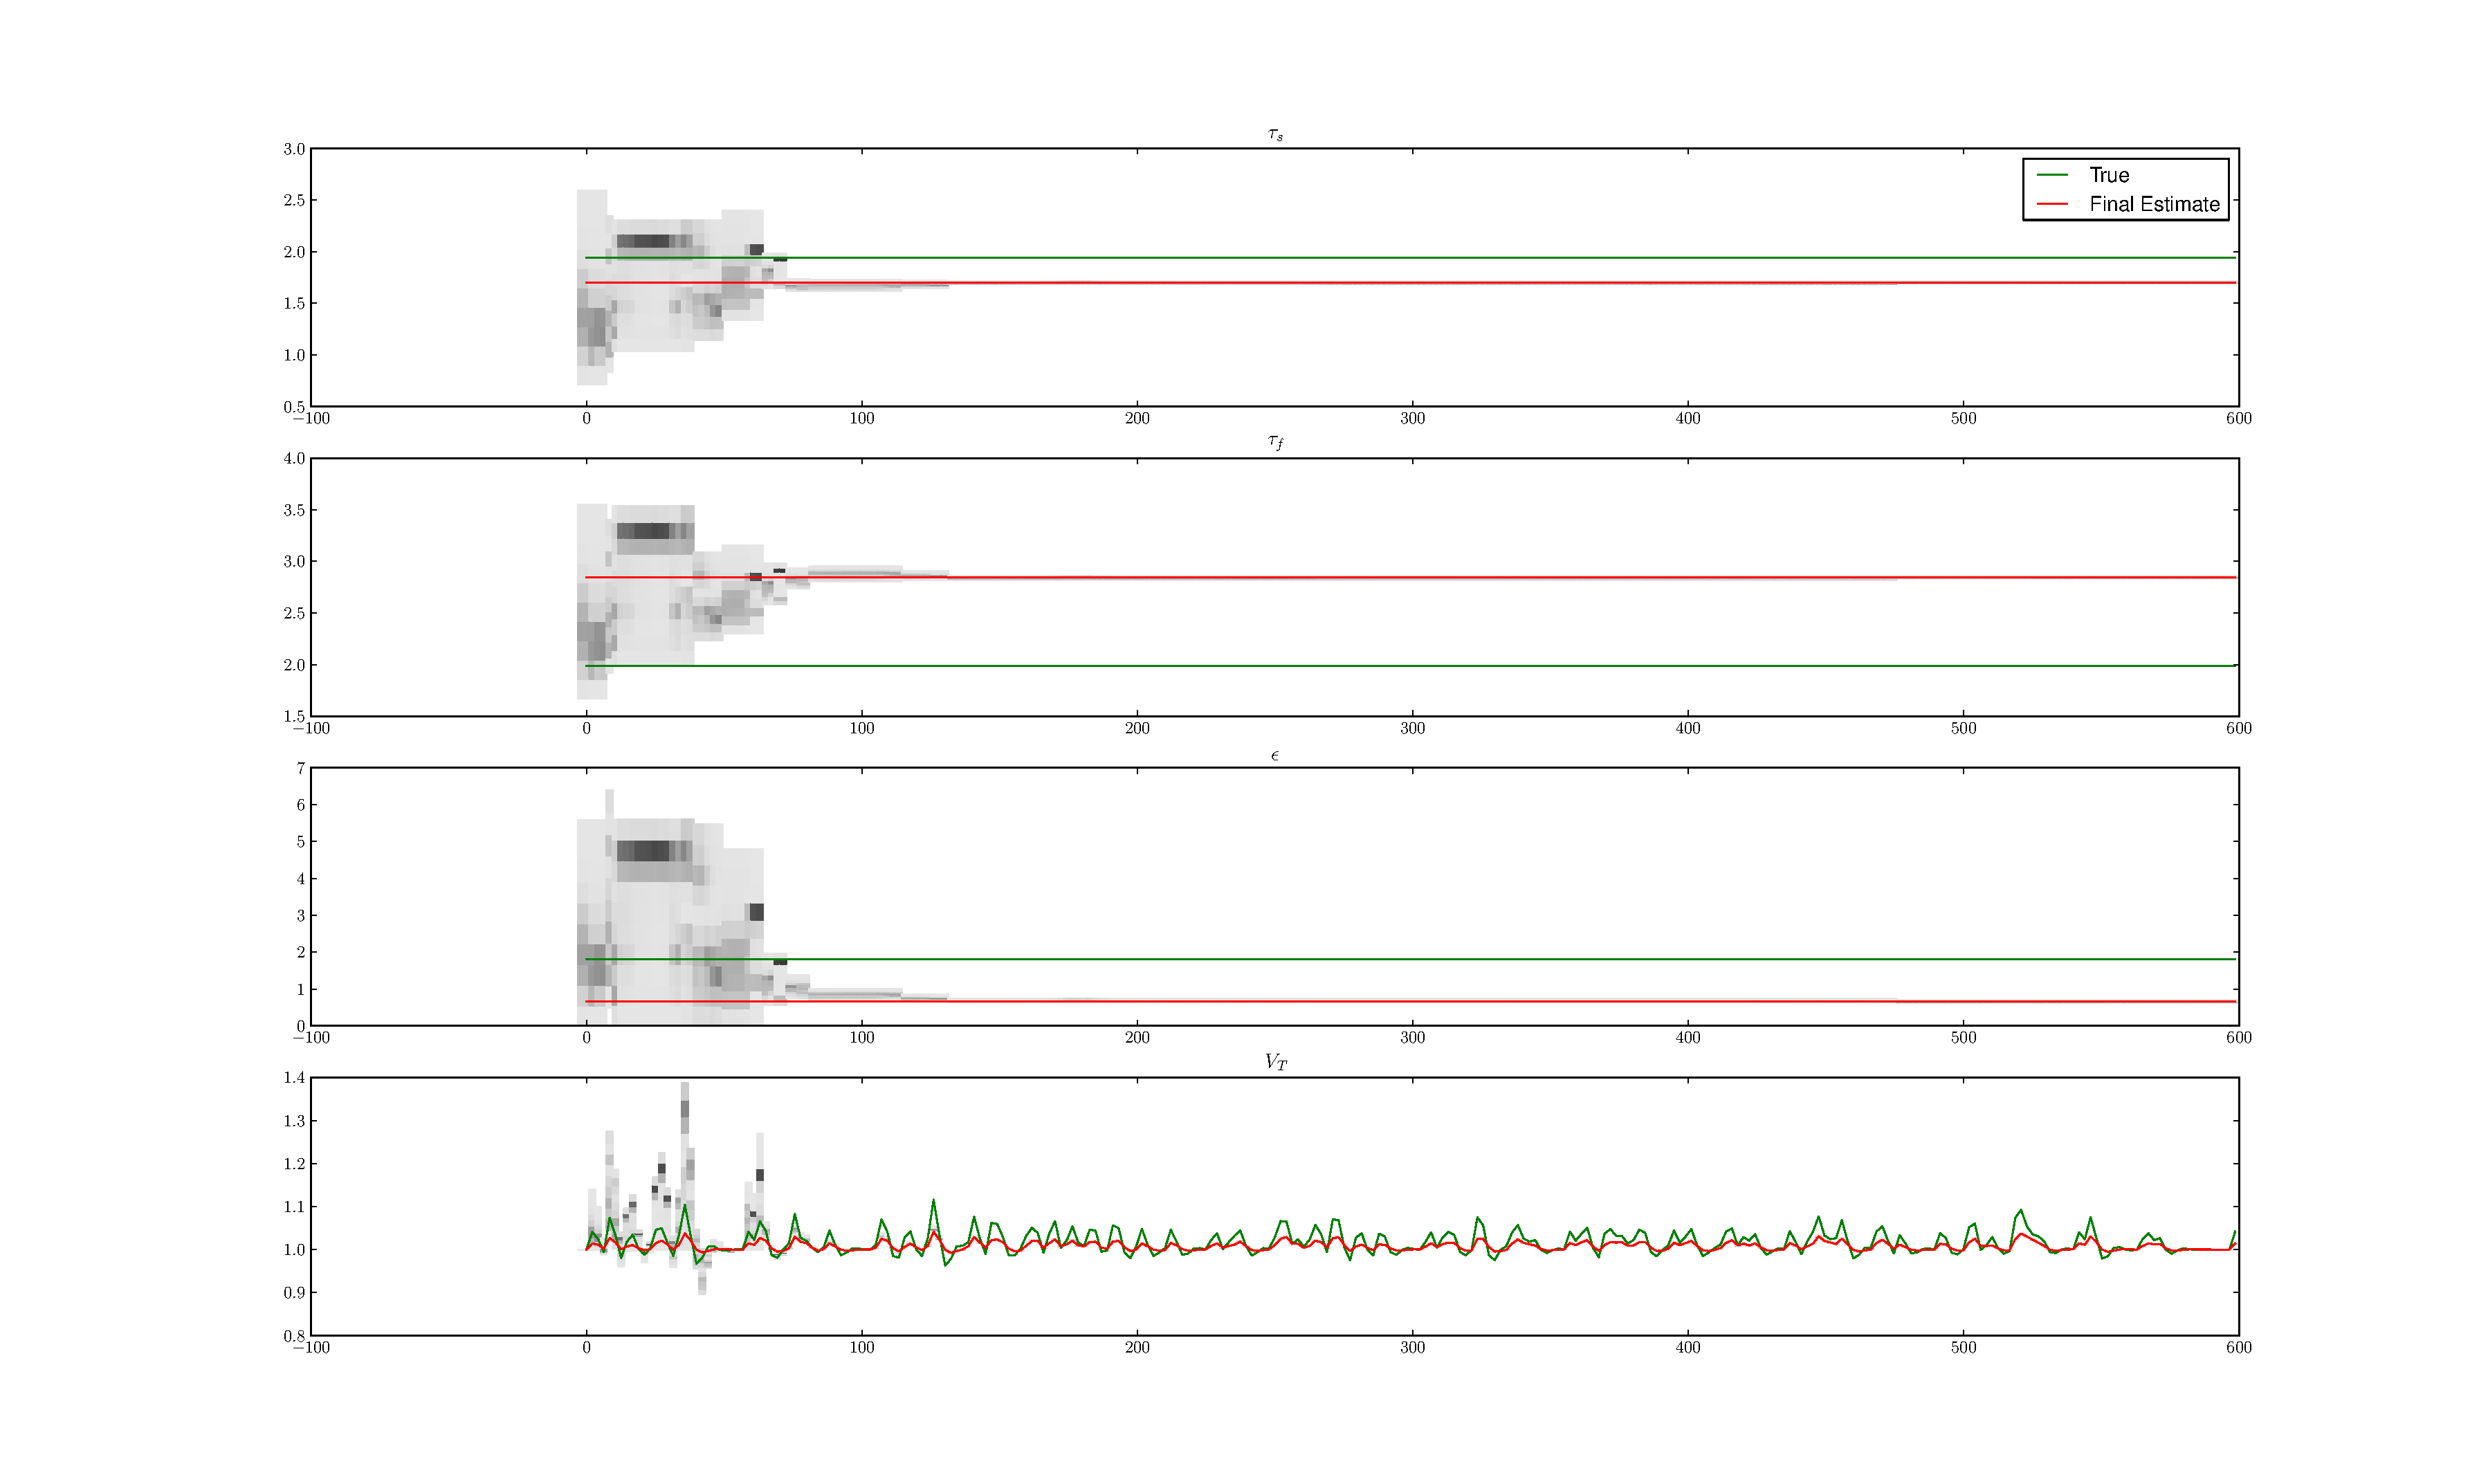
\includegraphics[clip=true,trim=6cm 2cm 6cm 3cm, width=\textwidth]{images/highnoise_run5_2}}
\end{figure}

\begin{figure}[H]
\subfigure
{\label{fig:ConvergenceRuns1c} 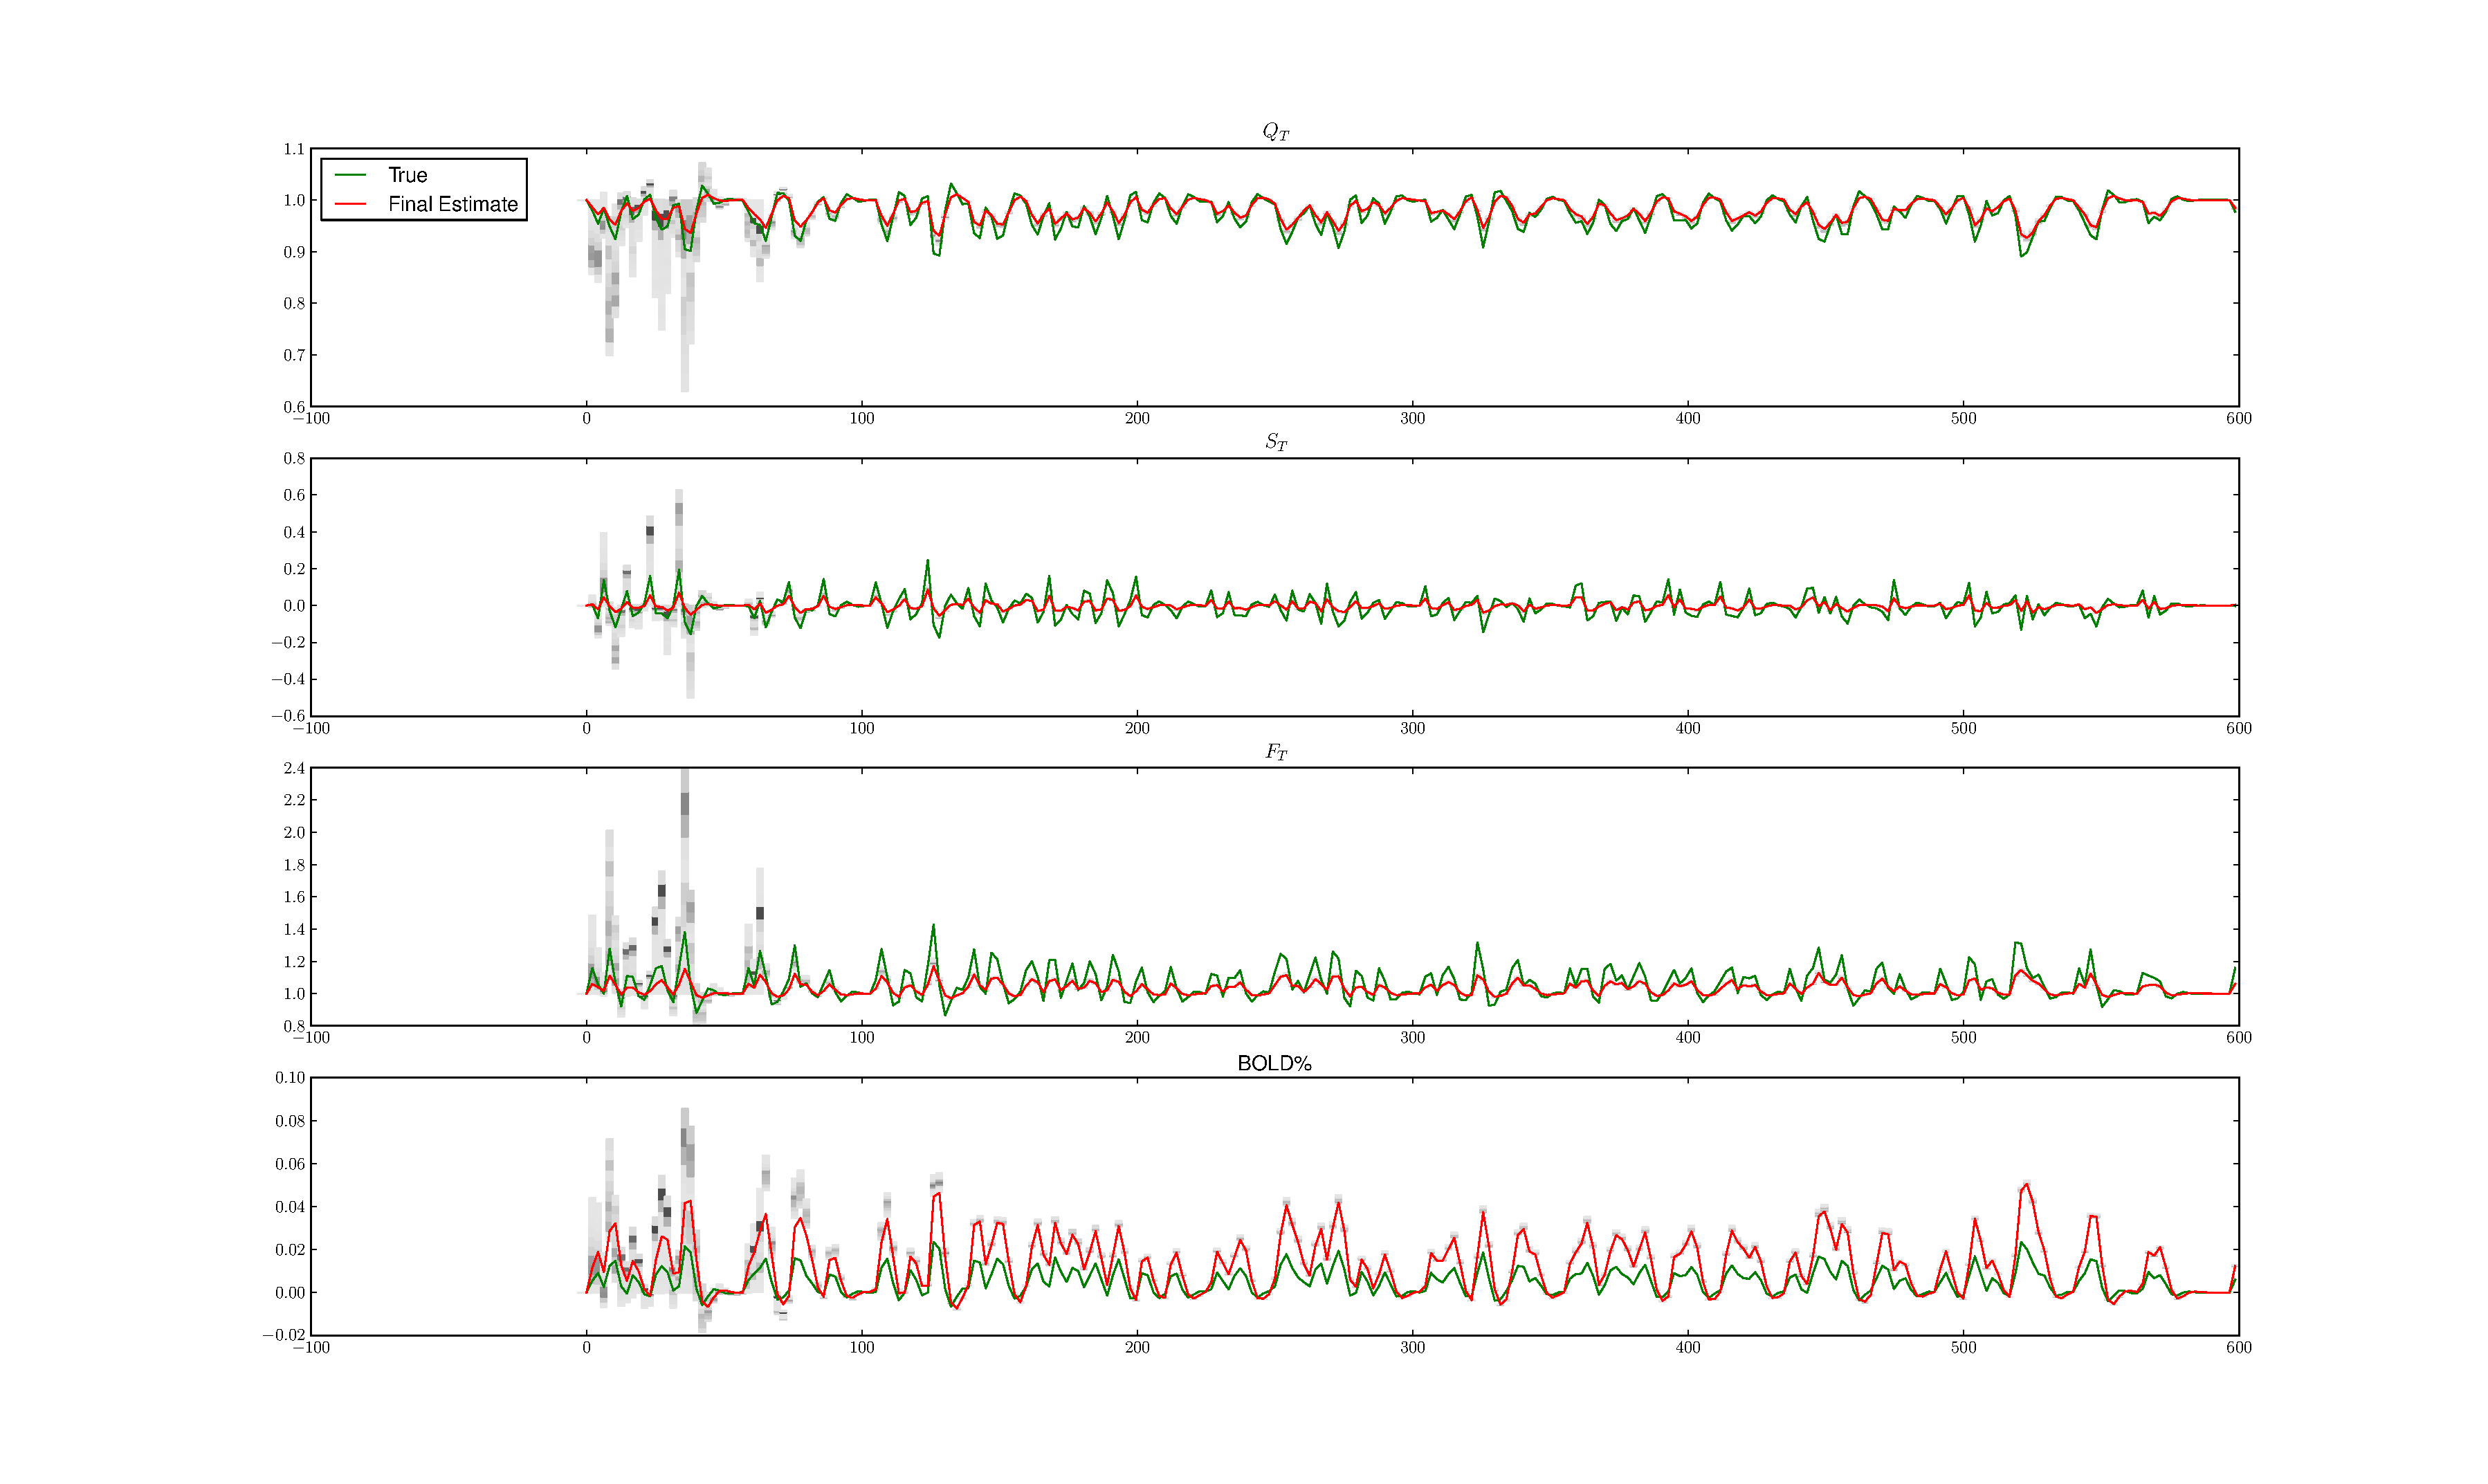
\includegraphics[clip=true,trim=6cm 2cm 6cm 3cm, width=\textwidth]{images/highnoise_run5_3}}
\caption[Convergence of the parameters during run 1 of \autoref{fig:NoiseComparisonJustTwo}]
{Convergence of the parameters during run 1 of \autoref{fig:NoiseComparisonJustTwo}.
Order of estimates: $\tau_0, \alpha, E_0, V_0, \tau_s, \tau_f, \epsilon, v,
q, s, f, BOLD$.  The bars represent
a histogram, where darker bars indicate more particles with parameters in that bin. The red 
line is the parameter used to generate the true signal, blue line is the final mean of the
particles.}
\label{fig:ConvergenceRuns1}
\end{figure}

\begin{figure}[H]
\subfigure
{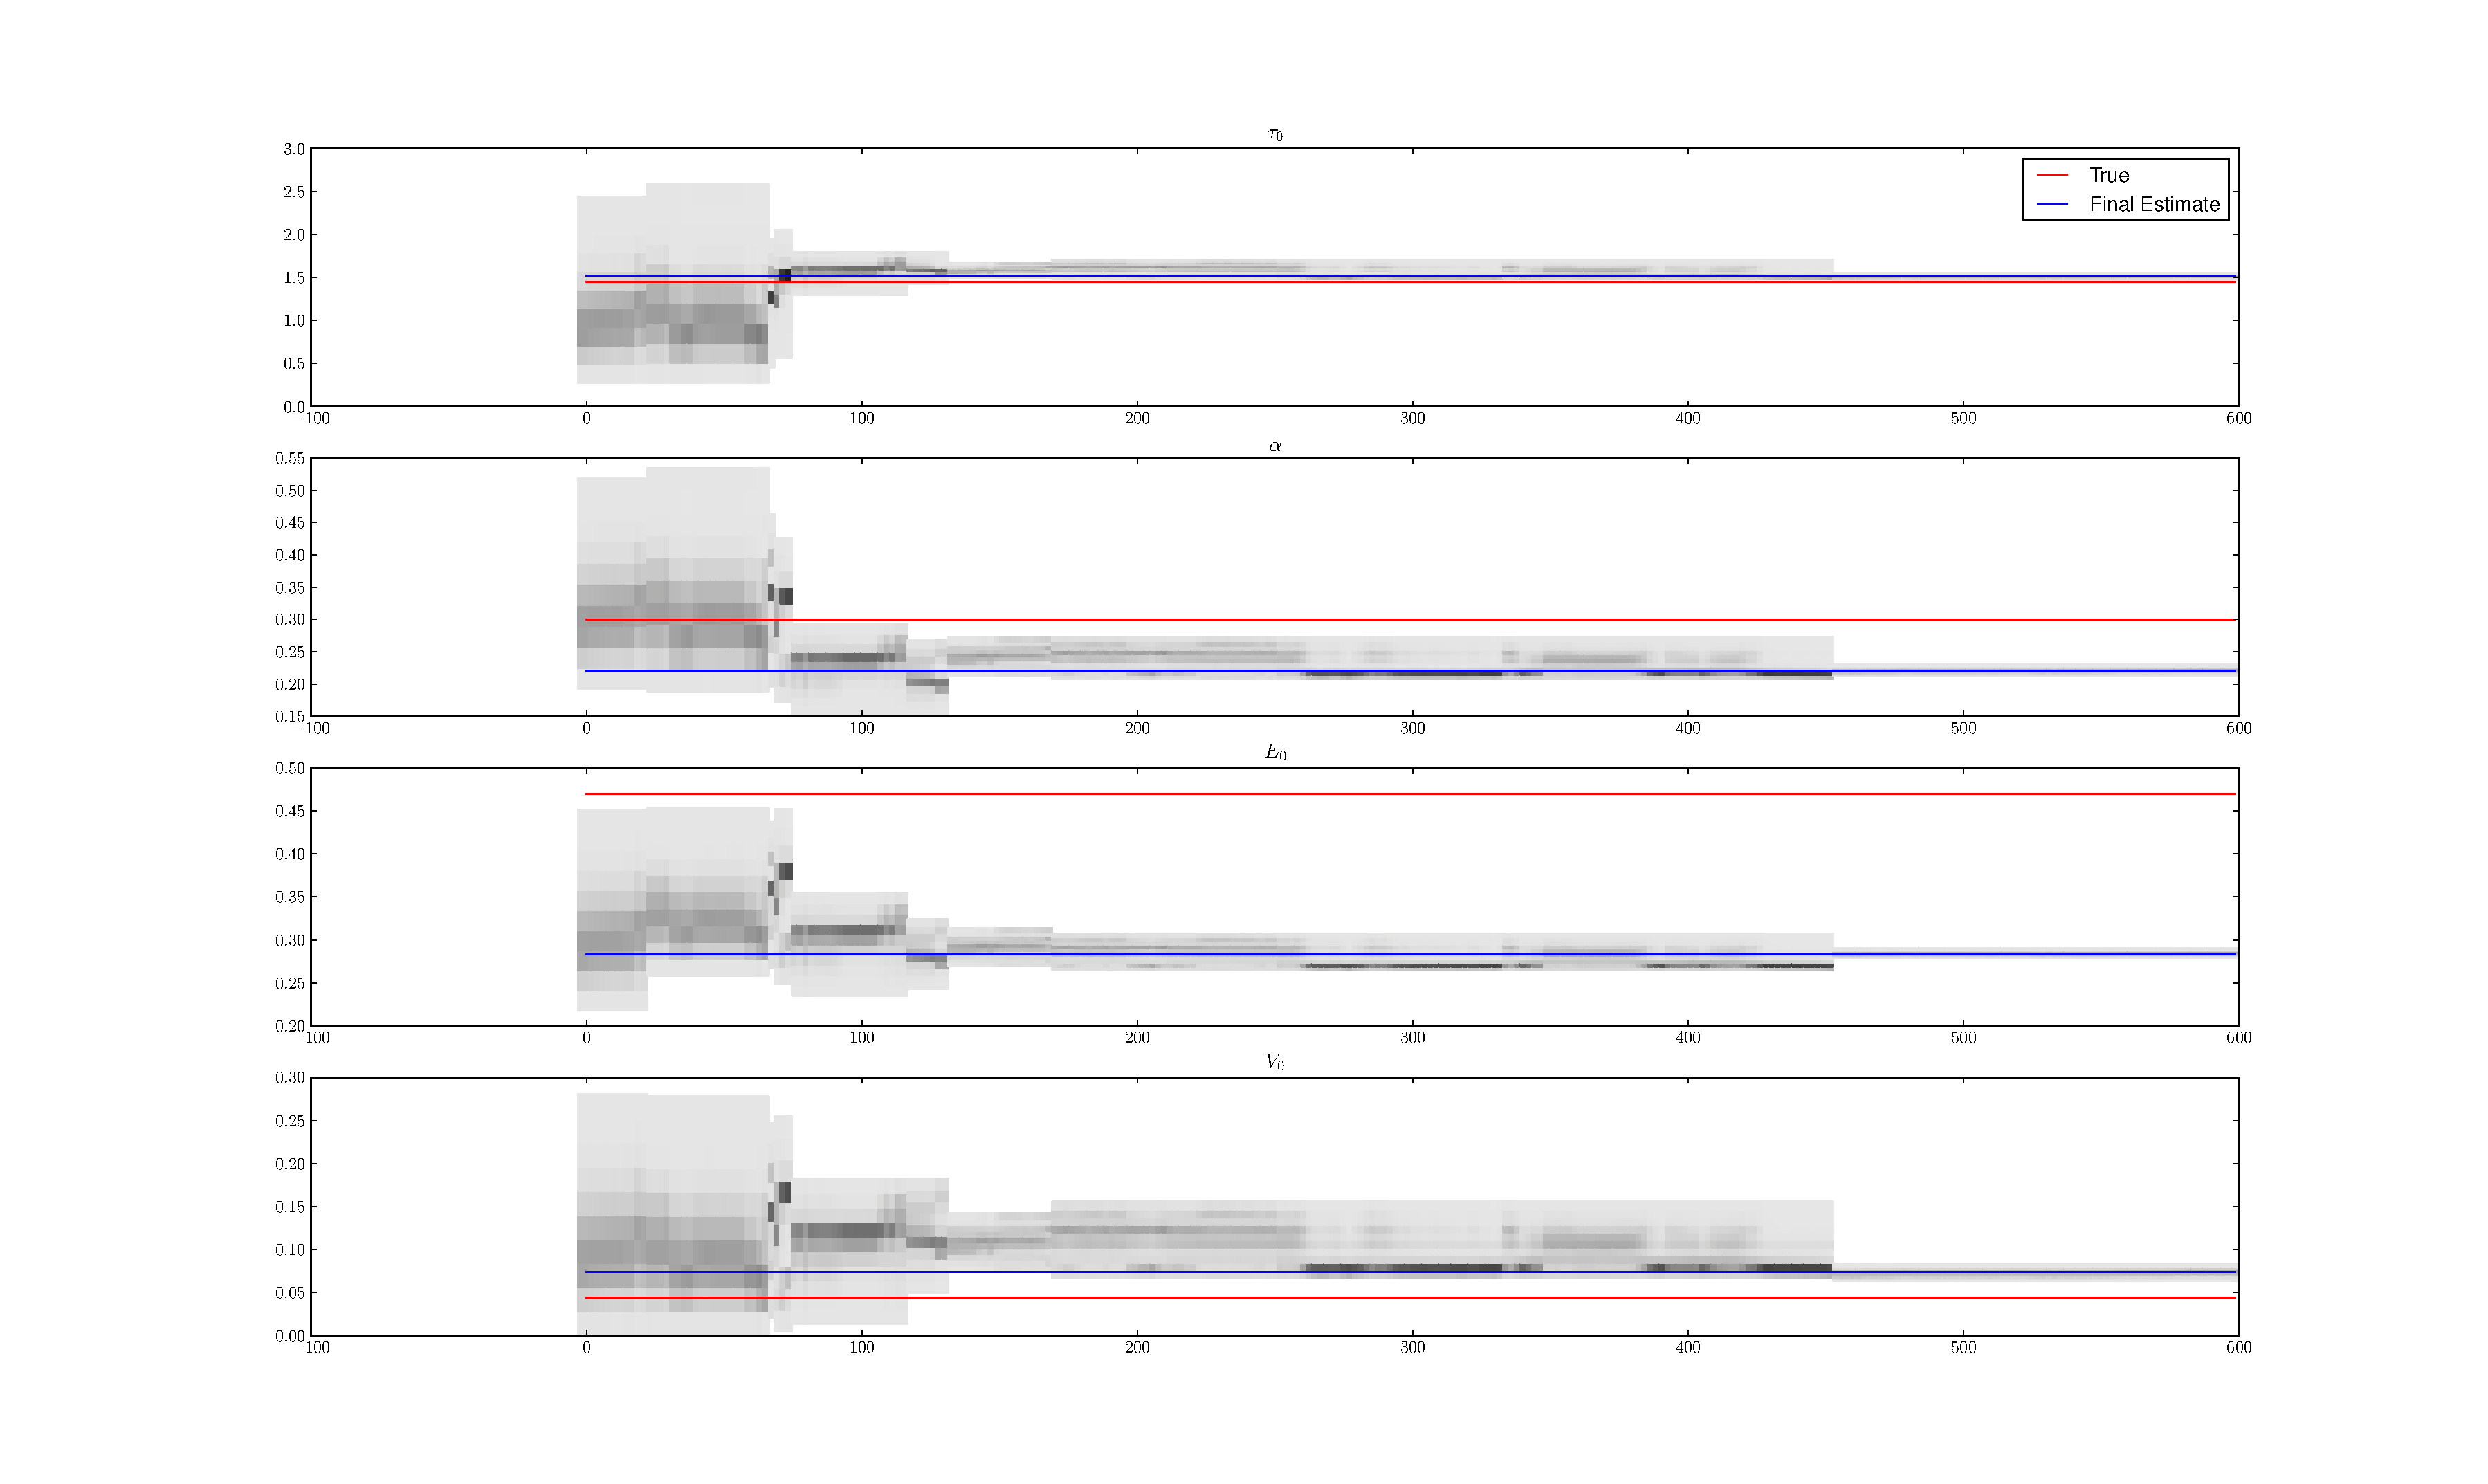
\includegraphics[clip=true,trim=6cm 2cm 6cm 3cm, width=\textwidth]{images/highnoise_run6_1}}
\subfigure
{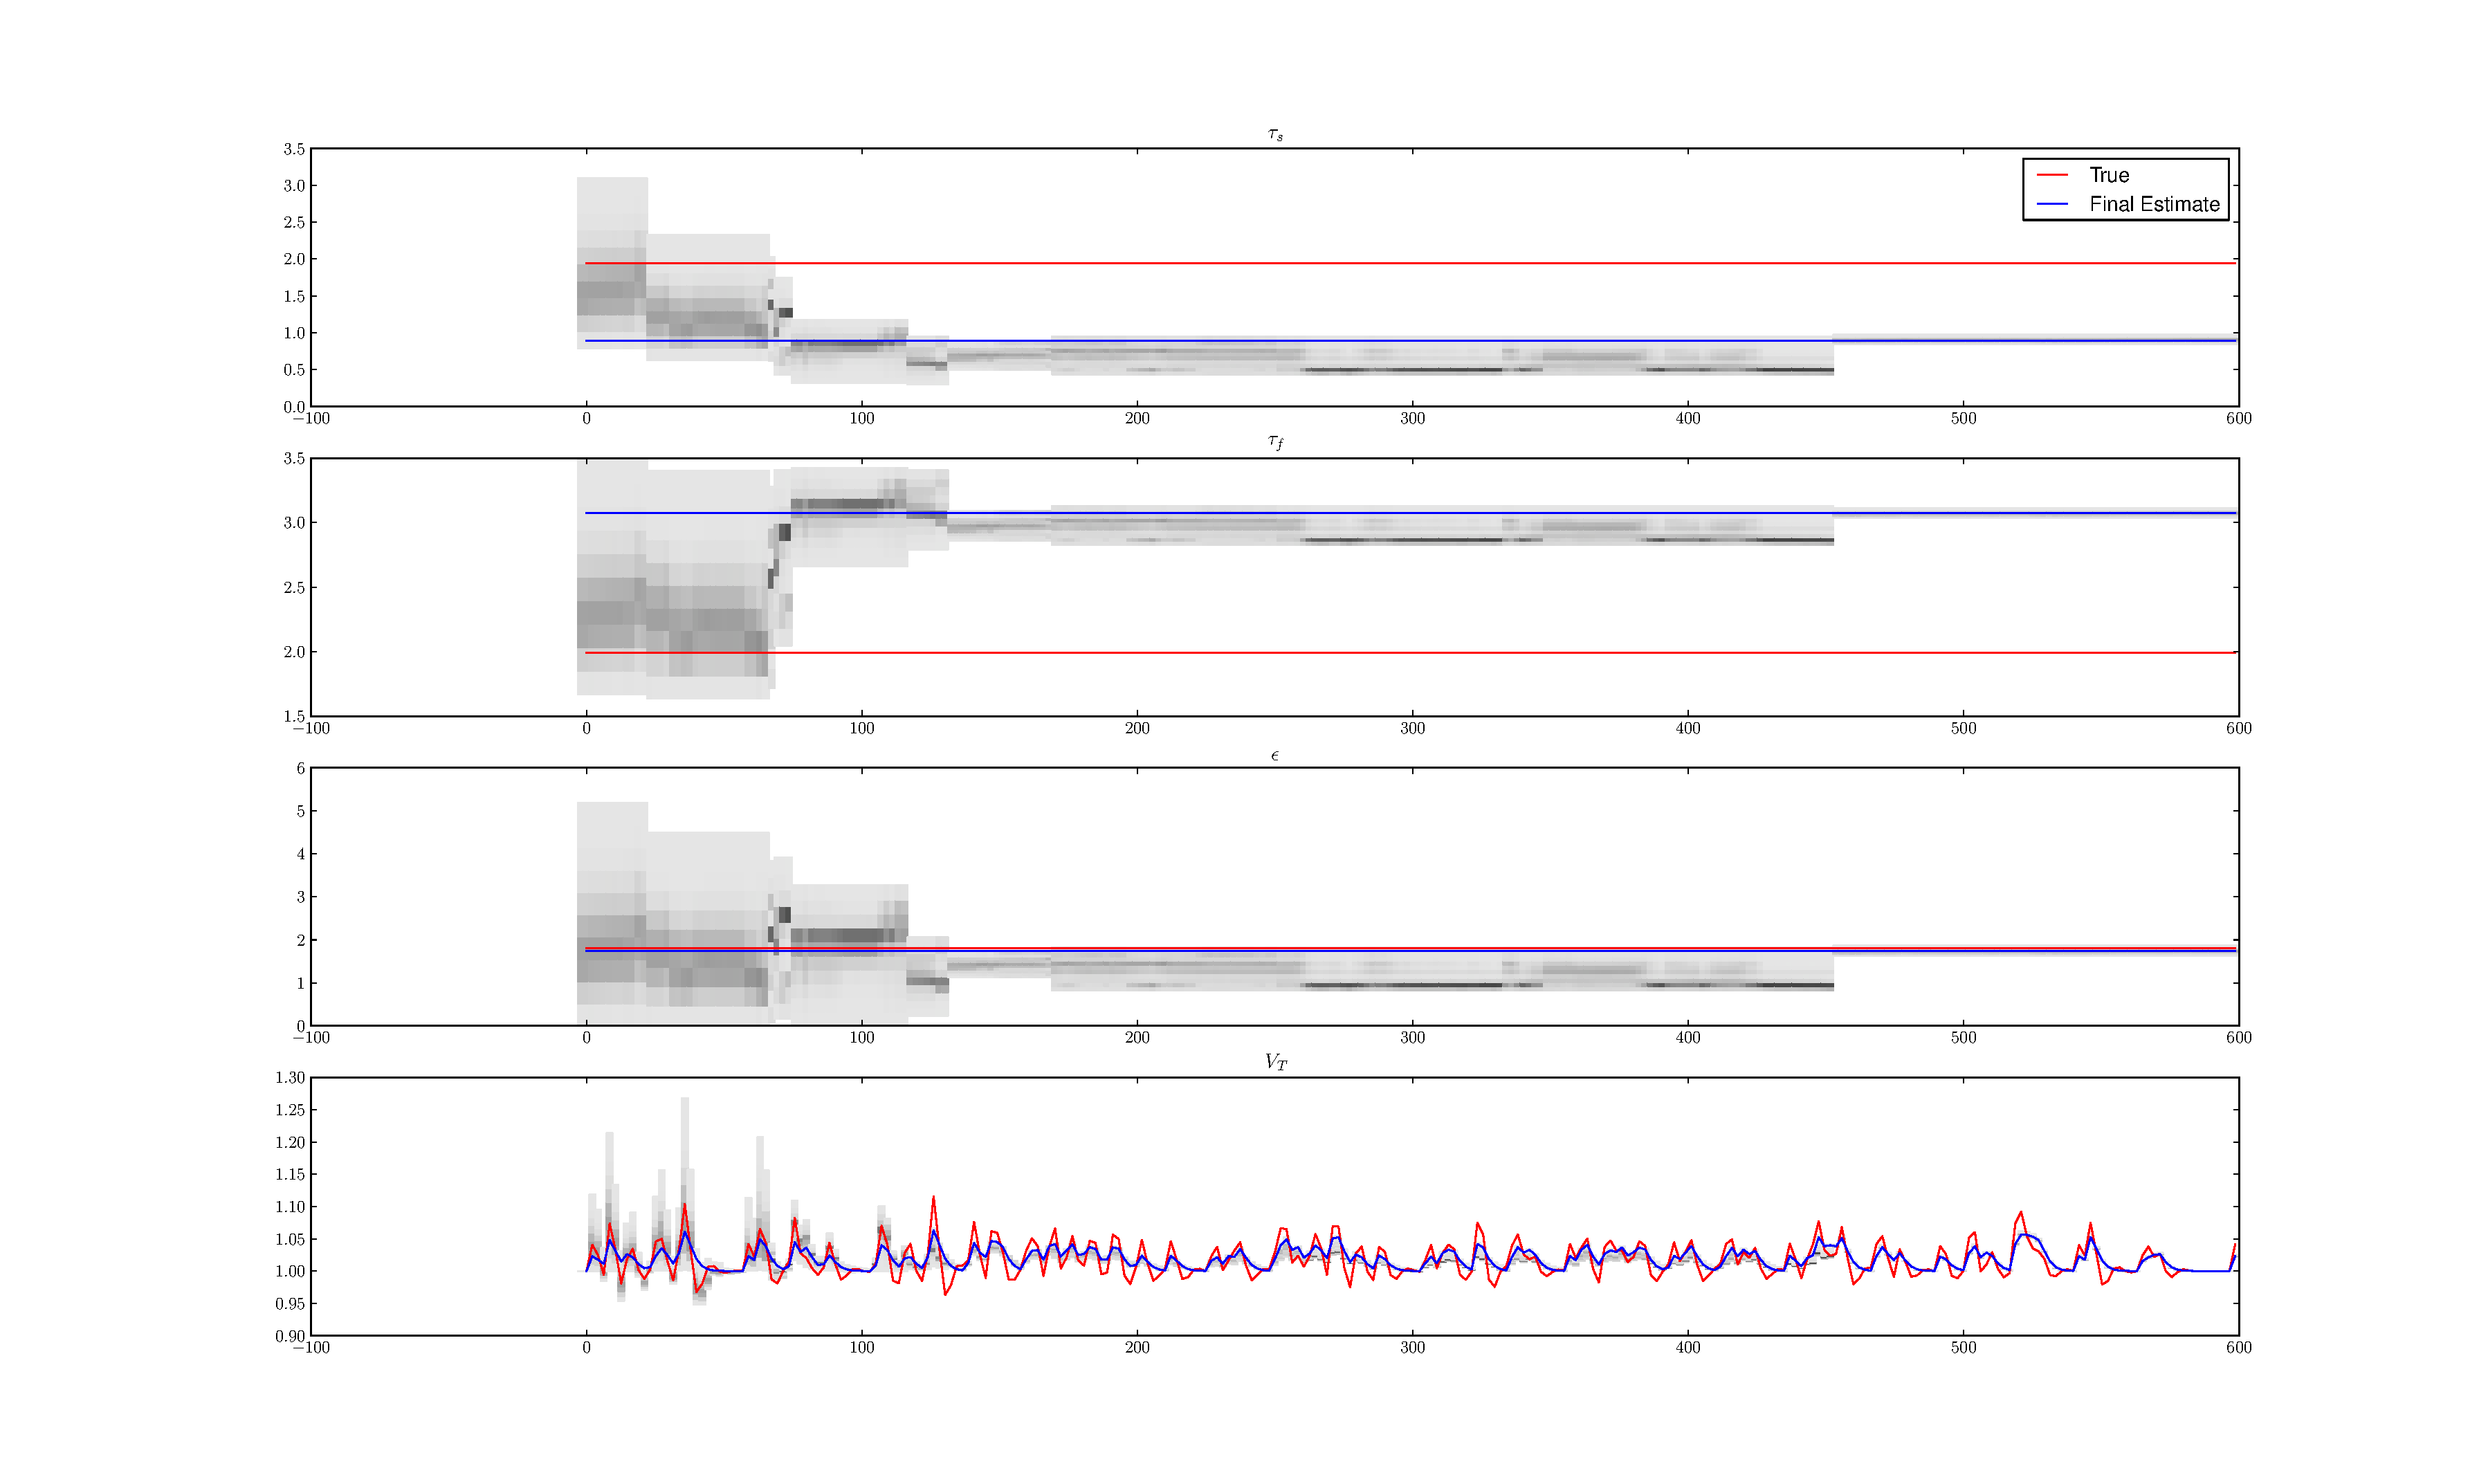
\includegraphics[clip=true,trim=6cm 2cm 6cm 3cm, width=\textwidth]{images/highnoise_run6_2}}
\end{figure}

\begin{figure}[H]
\subfigure
{\label{fig:ConvergenceRuns2c} 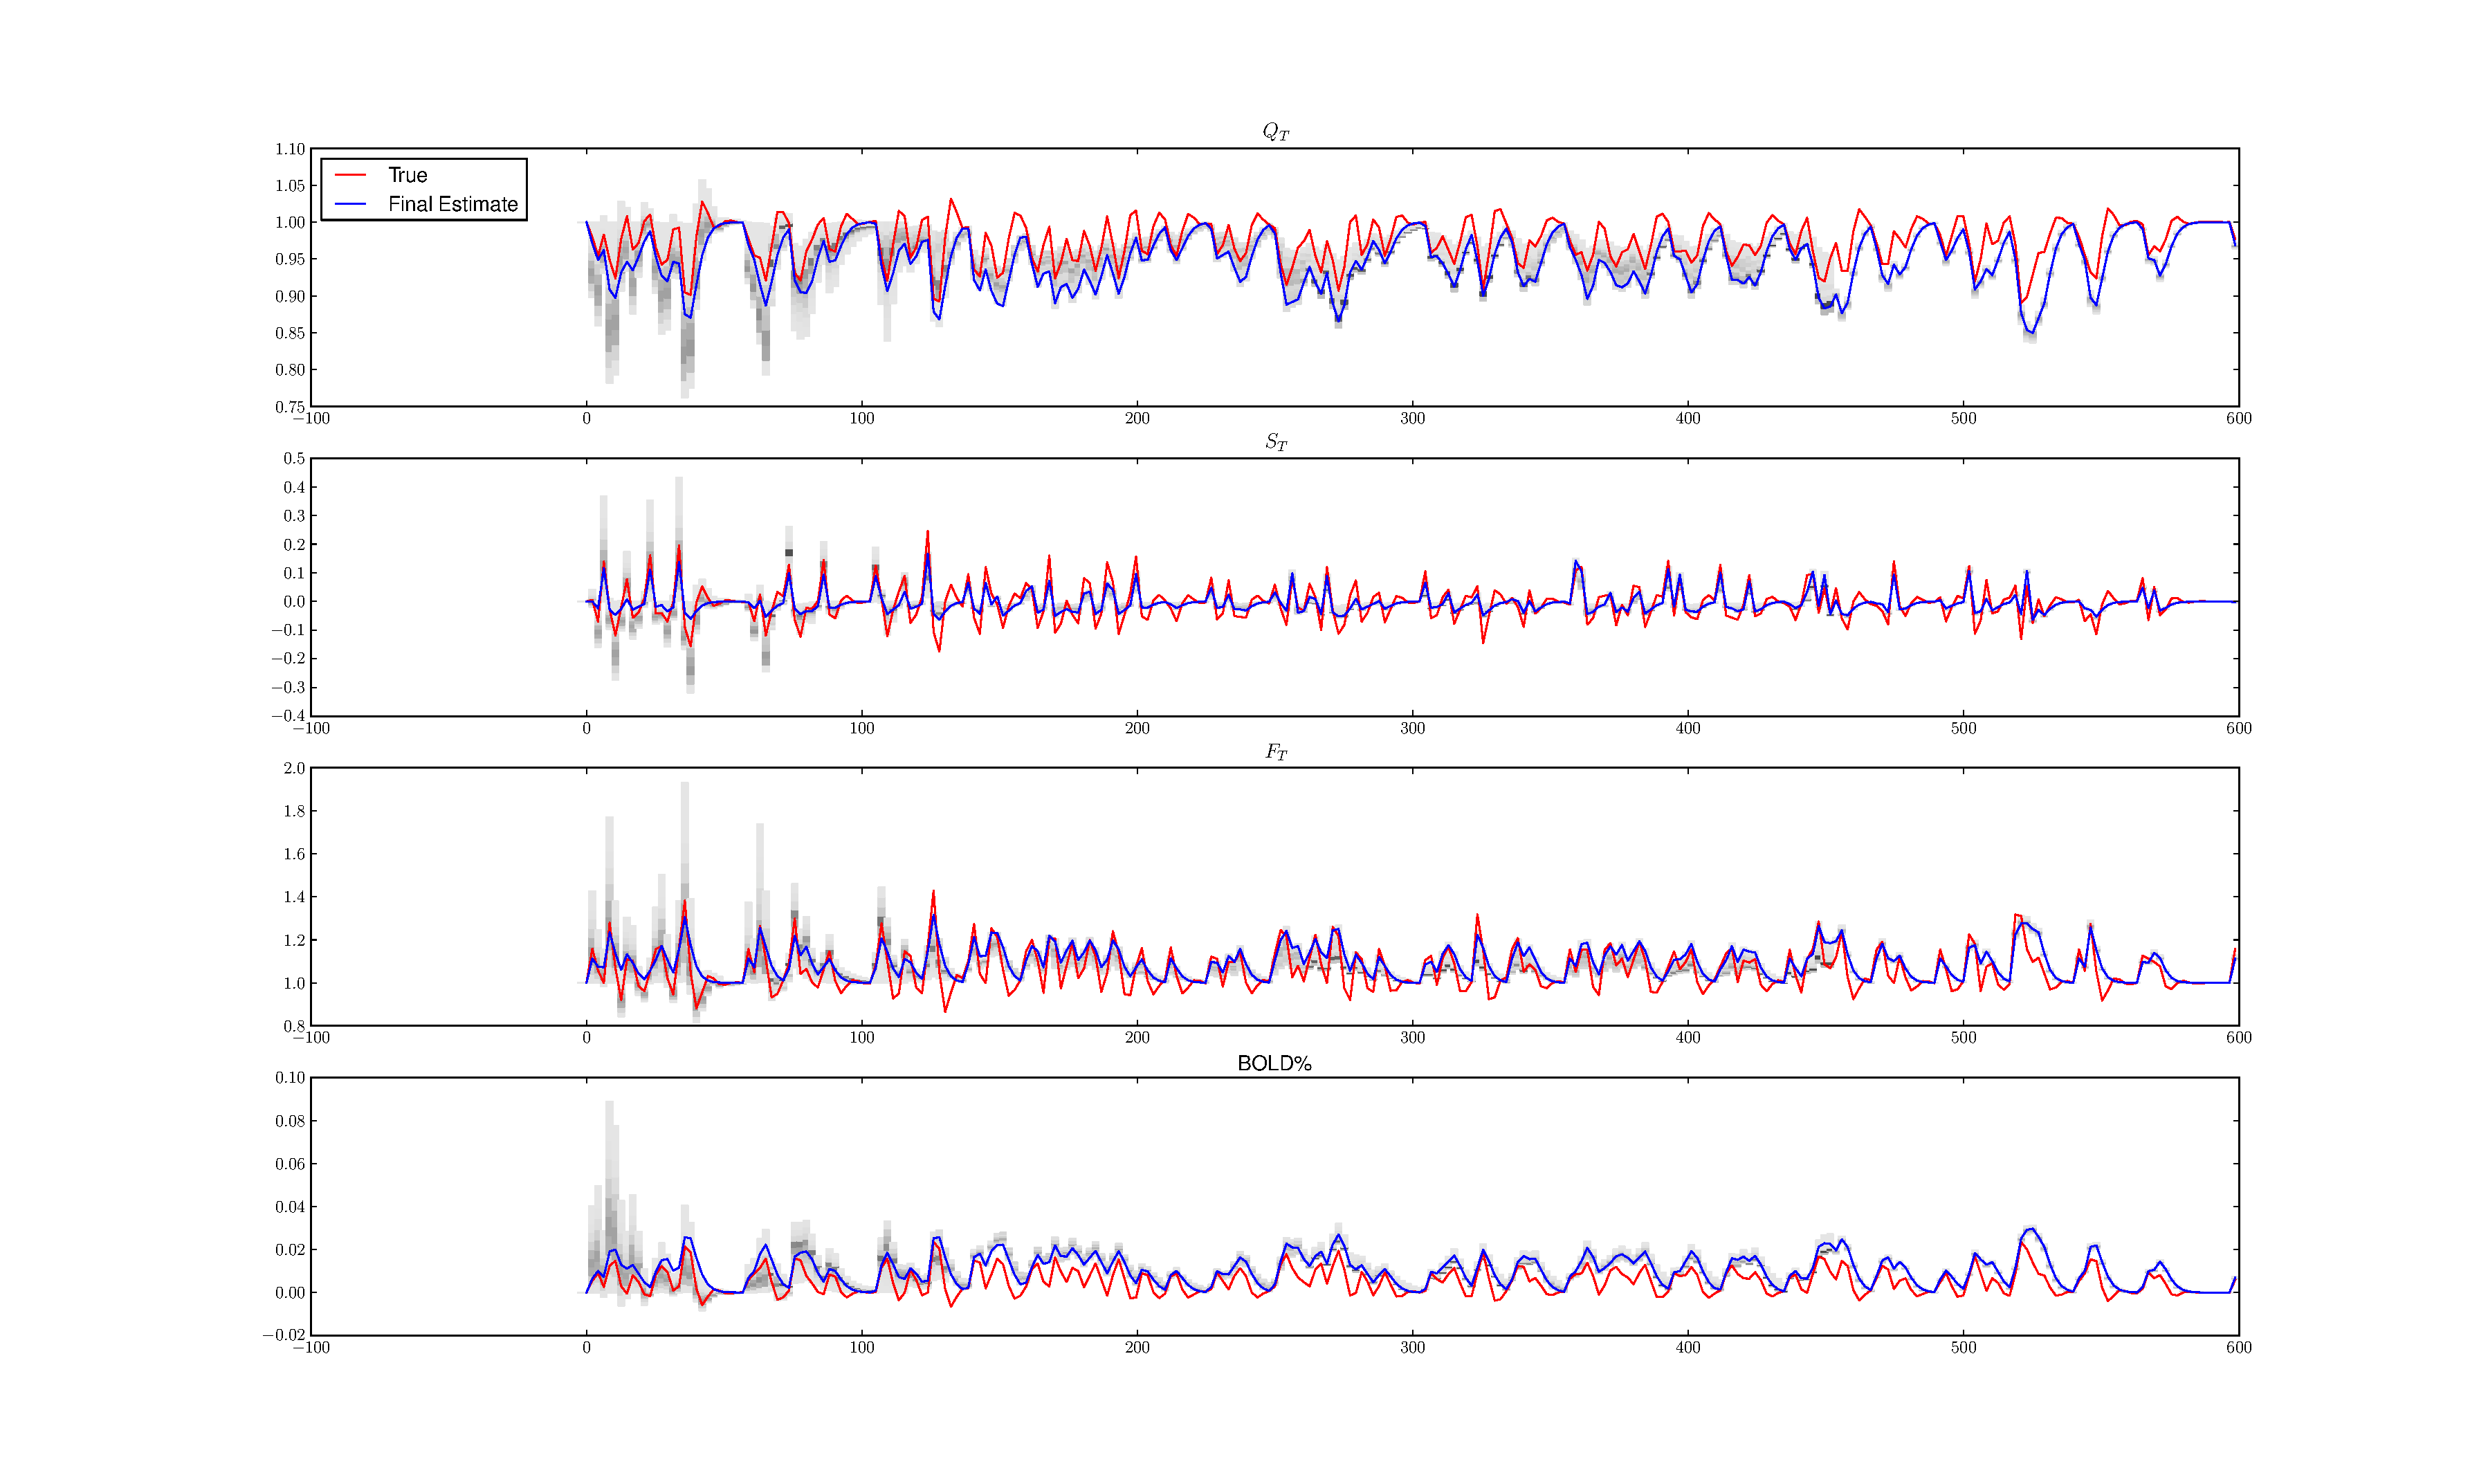
\includegraphics[clip=true,trim=6cm 2cm 6cm 3cm, width=\textwidth]{images/highnoise_run6_3}}
\caption[Convergence of the parameters during run 2 of \autoref{fig:NoiseComparisonJustTwo}]
{Convergence of the parameters during run 2 of \autoref{fig:NoiseComparisonJustTwo}.
Order of estimates: $\tau_0, \alpha, E_0, V_0, \tau_s, \tau_f, \epsilon, v,
q, s, f, BOLD$.  The bars represent
a histogram, where darker bars indicate more particles with parameters in that bin. The red 
line is the parameter used to generate the true signal, blue line is the final mean of the
particles.}
\label{fig:ConvergenceRuns2}
\end{figure}

The particles converged much faster when more noise was present (\autoref{fig:LowNoiseHist} vs.
\autoref{fig:ConvergenceRuns1}, \autoref{fig:ConvergenceRuns2}).
This also caused significantly more resampling which
is the explanation for the perceived jumps in the histograms.
Clearly the additional noise resulted in less consistent results 
(\autoref{tab:HighNoiseResults}).
This is often the
result when the particle filter converges too fast, in this case the result of the
weighting function's variance being smaller than the measurement noise ($0.005$ vs. $0.01$).
The \ac{RMSE} clearly suffers due to this effect (\autoref{tab:HighNoiseResults}).
Note that neither Run 1 nor Run 2 estimated the underlying state well (\autoref{fig:ConvergenceRuns1c}
and \autoref{fig:ConvergenceRuns2c}), whereas
in the previous test the particle filter was extremely successful in this area (\autoref{fig:LowNoiseHistc}).

%NO SIGNAL, LOW NOISE
\subsection{Pure Noise, Low magnitude}
\label{sec:PureNoiseLowMag}
The next two single-voxel tests forced the particle filter to attempt to learn a noise-only
time series. In this test the noise was the same as that from the \autoref{sec:SimHighNoise},
$\sigma_x = 0.01, \sigma_y = 0.005$. The stimulus neuronal efficiency ($\epsilon$) was set
to 0, in effect simulating a brain region with no response to the stimuli.
This test was used to determine how the output of a pure noise time series
is different from that of a simple noisy signal (as in the previous two sections).
The preprocessed signals are shown in \autoref{fig:PreprocessedNoiseOnly}
and line fit for each run is shown in \autoref{fig:fits_noiseonly}.

%\begin{figure}[H]
%\centering
%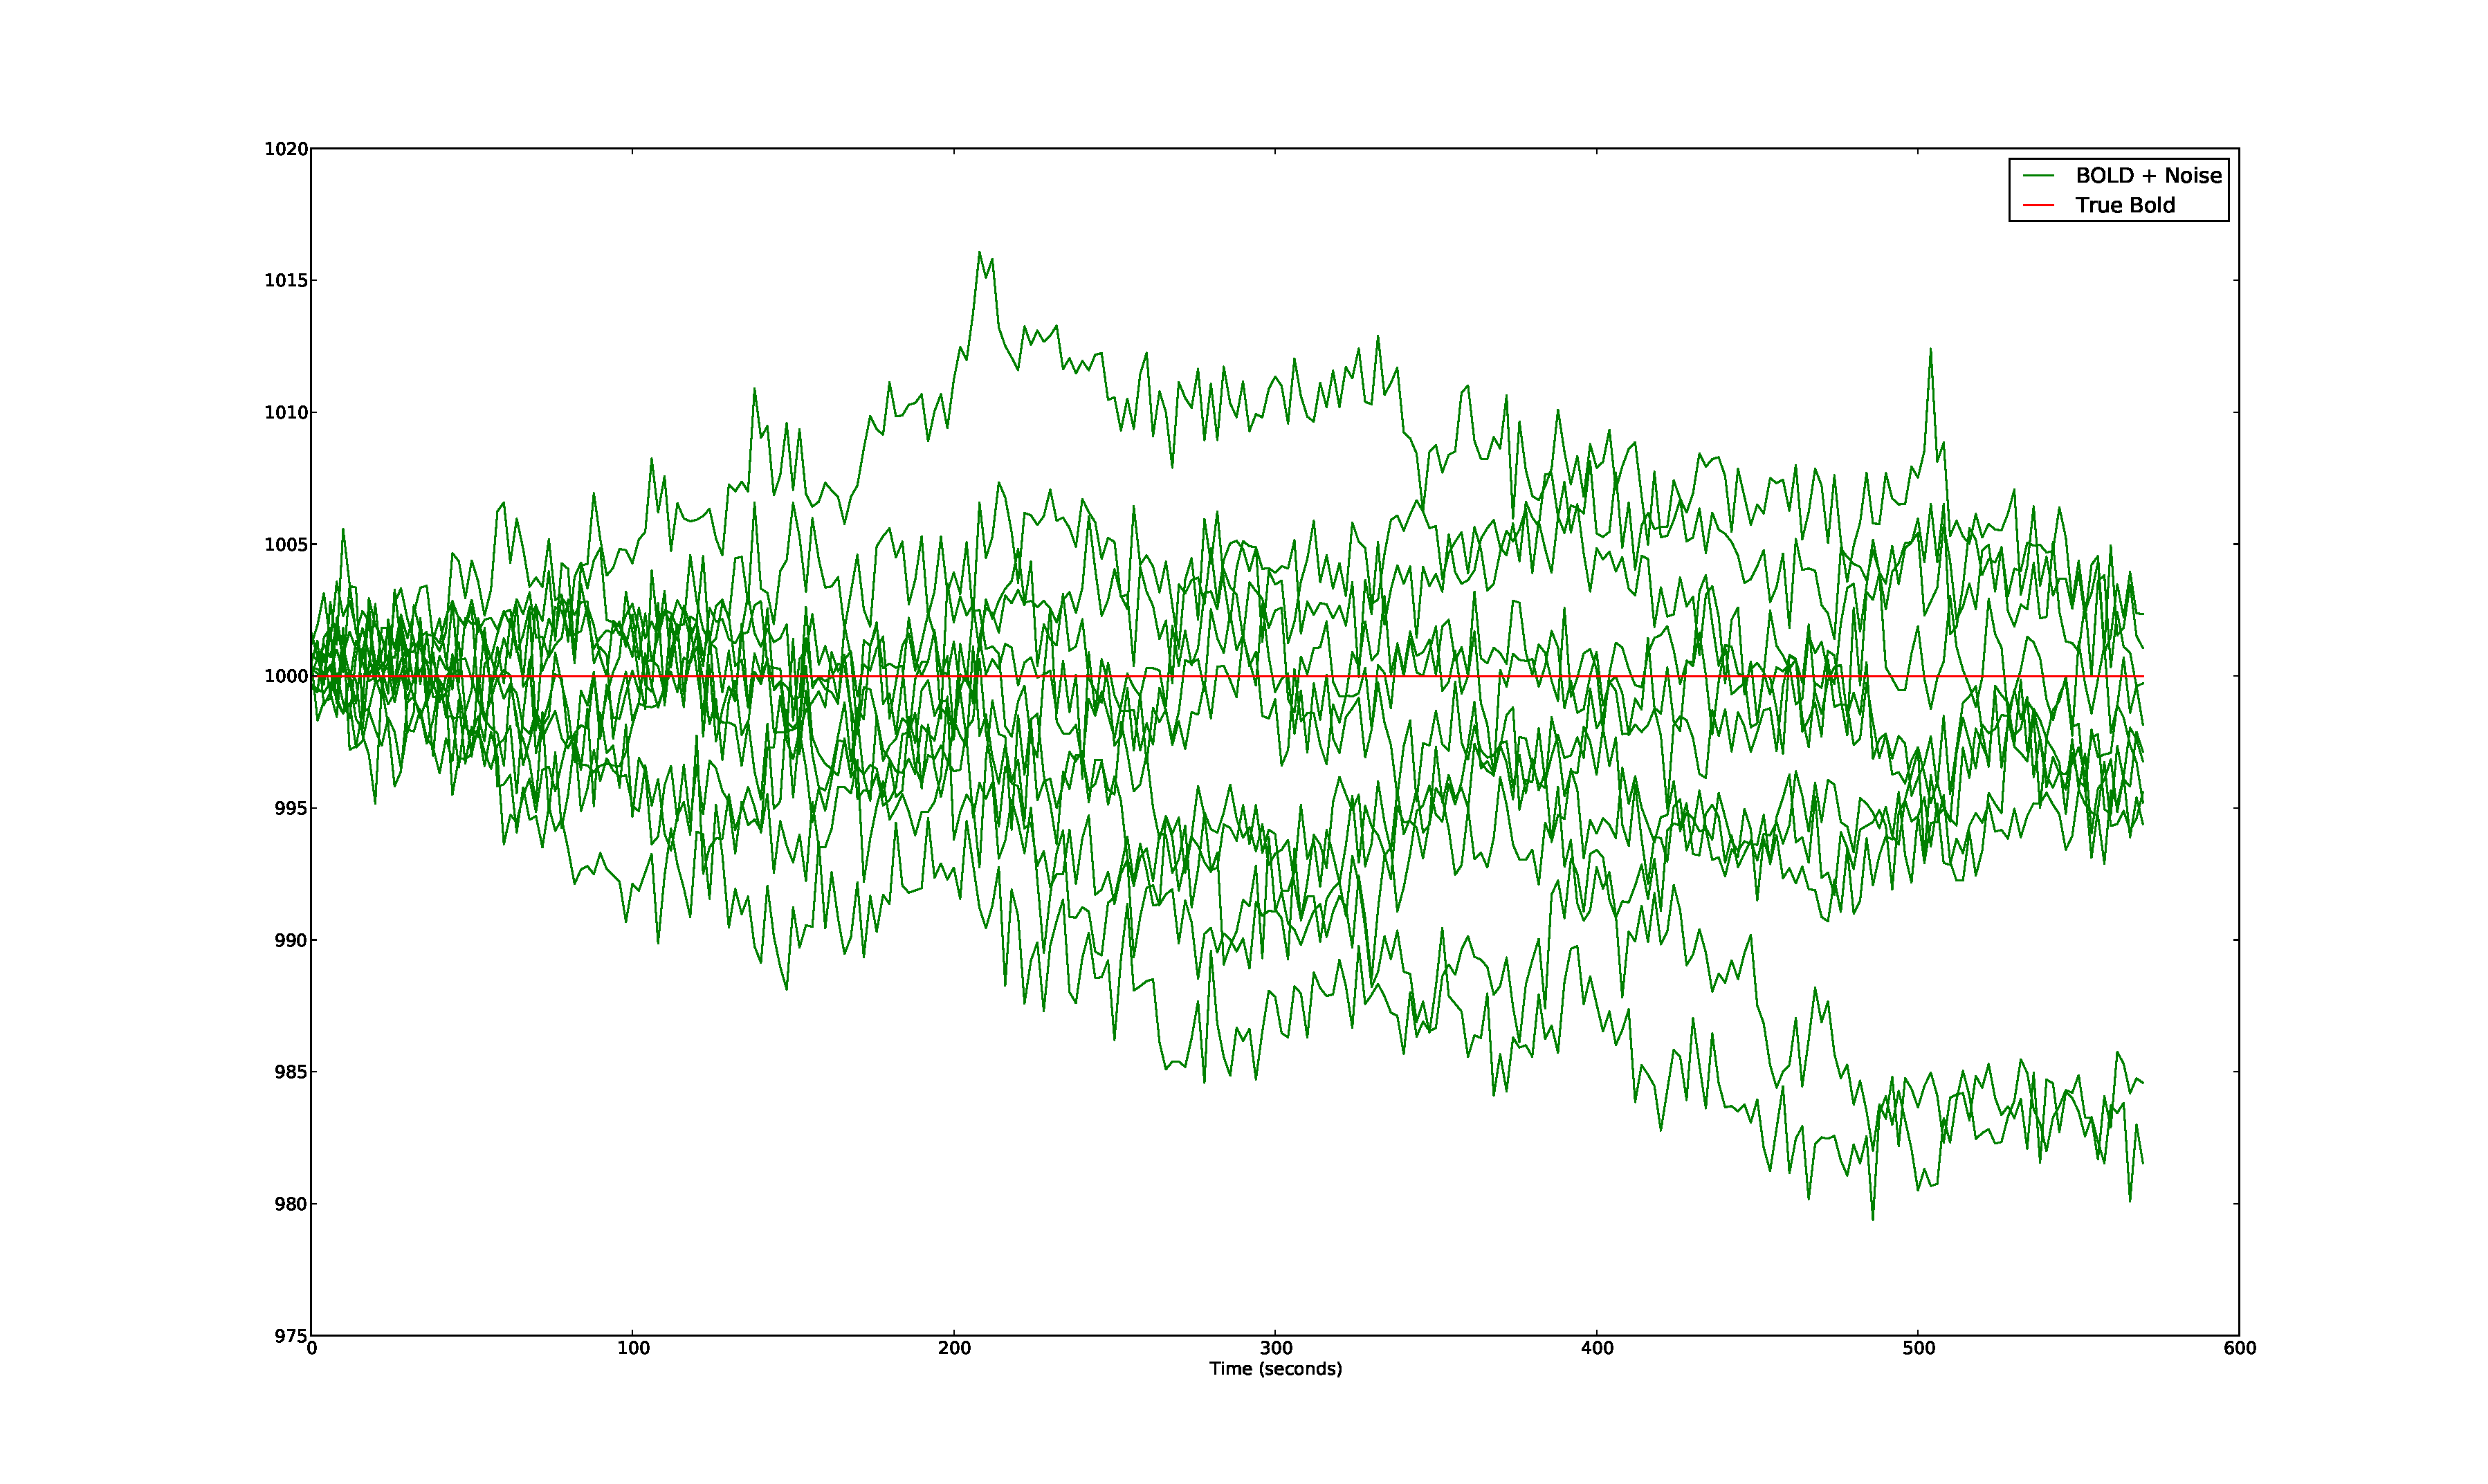
\includegraphics[clip=true,trim=6cm 3cm 6cm 3cm,height=7cm]{images/realization_noiseonly}
%\caption{Time-series lacking any real signal. With, ($\sigma_x = 0.01, \sigma_y=0.005$).}
%\label{fig:NoiseOnly}
%\end{figure}

\begin{figure}[H]
\centering
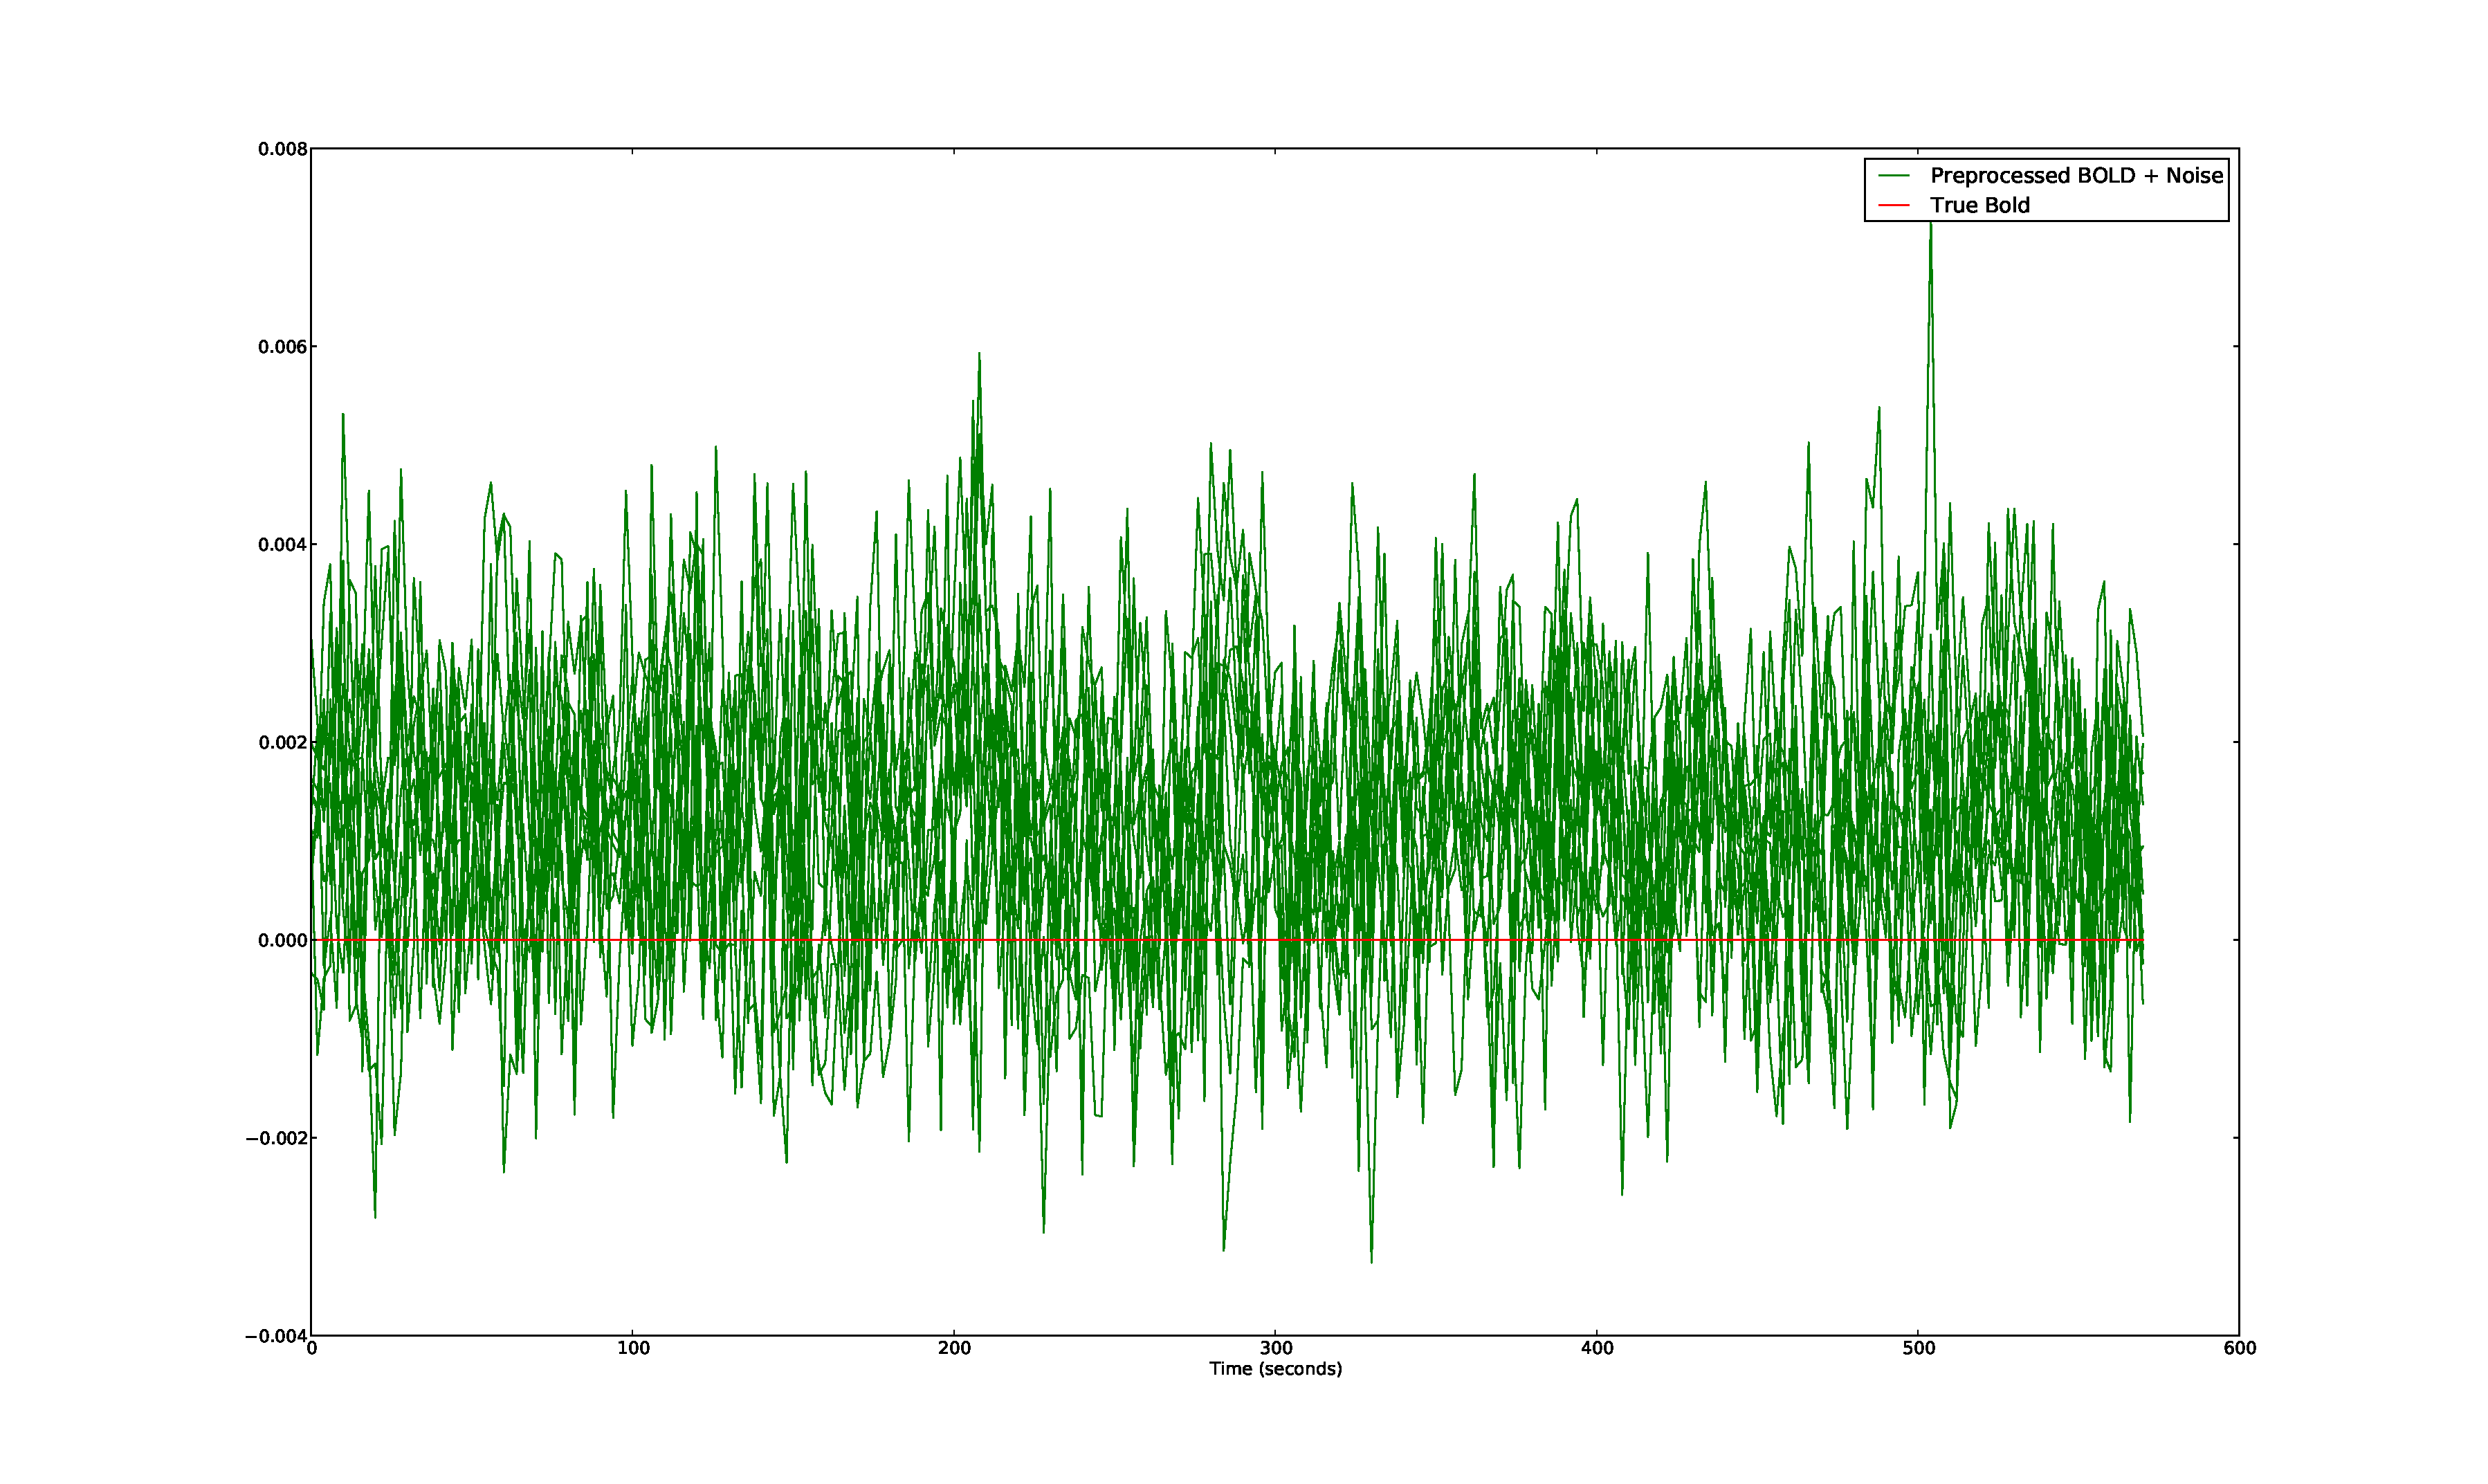
\includegraphics[clip=true,trim=6cm 2cm 6cm 3.5cm,width=15cm]{images/preprocessed_noiseonly}
\caption[Preprocessed Signal for non-active, low noise signal]
{Comparison of the preprocessed signals for the low noise signal-free case.
 ($\sigma_x = 0.005$, $\sigma_y = 0.01$)}
\label{fig:PreprocessedNoiseOnly}
\end{figure}

\begin{figure}[H]
\centering
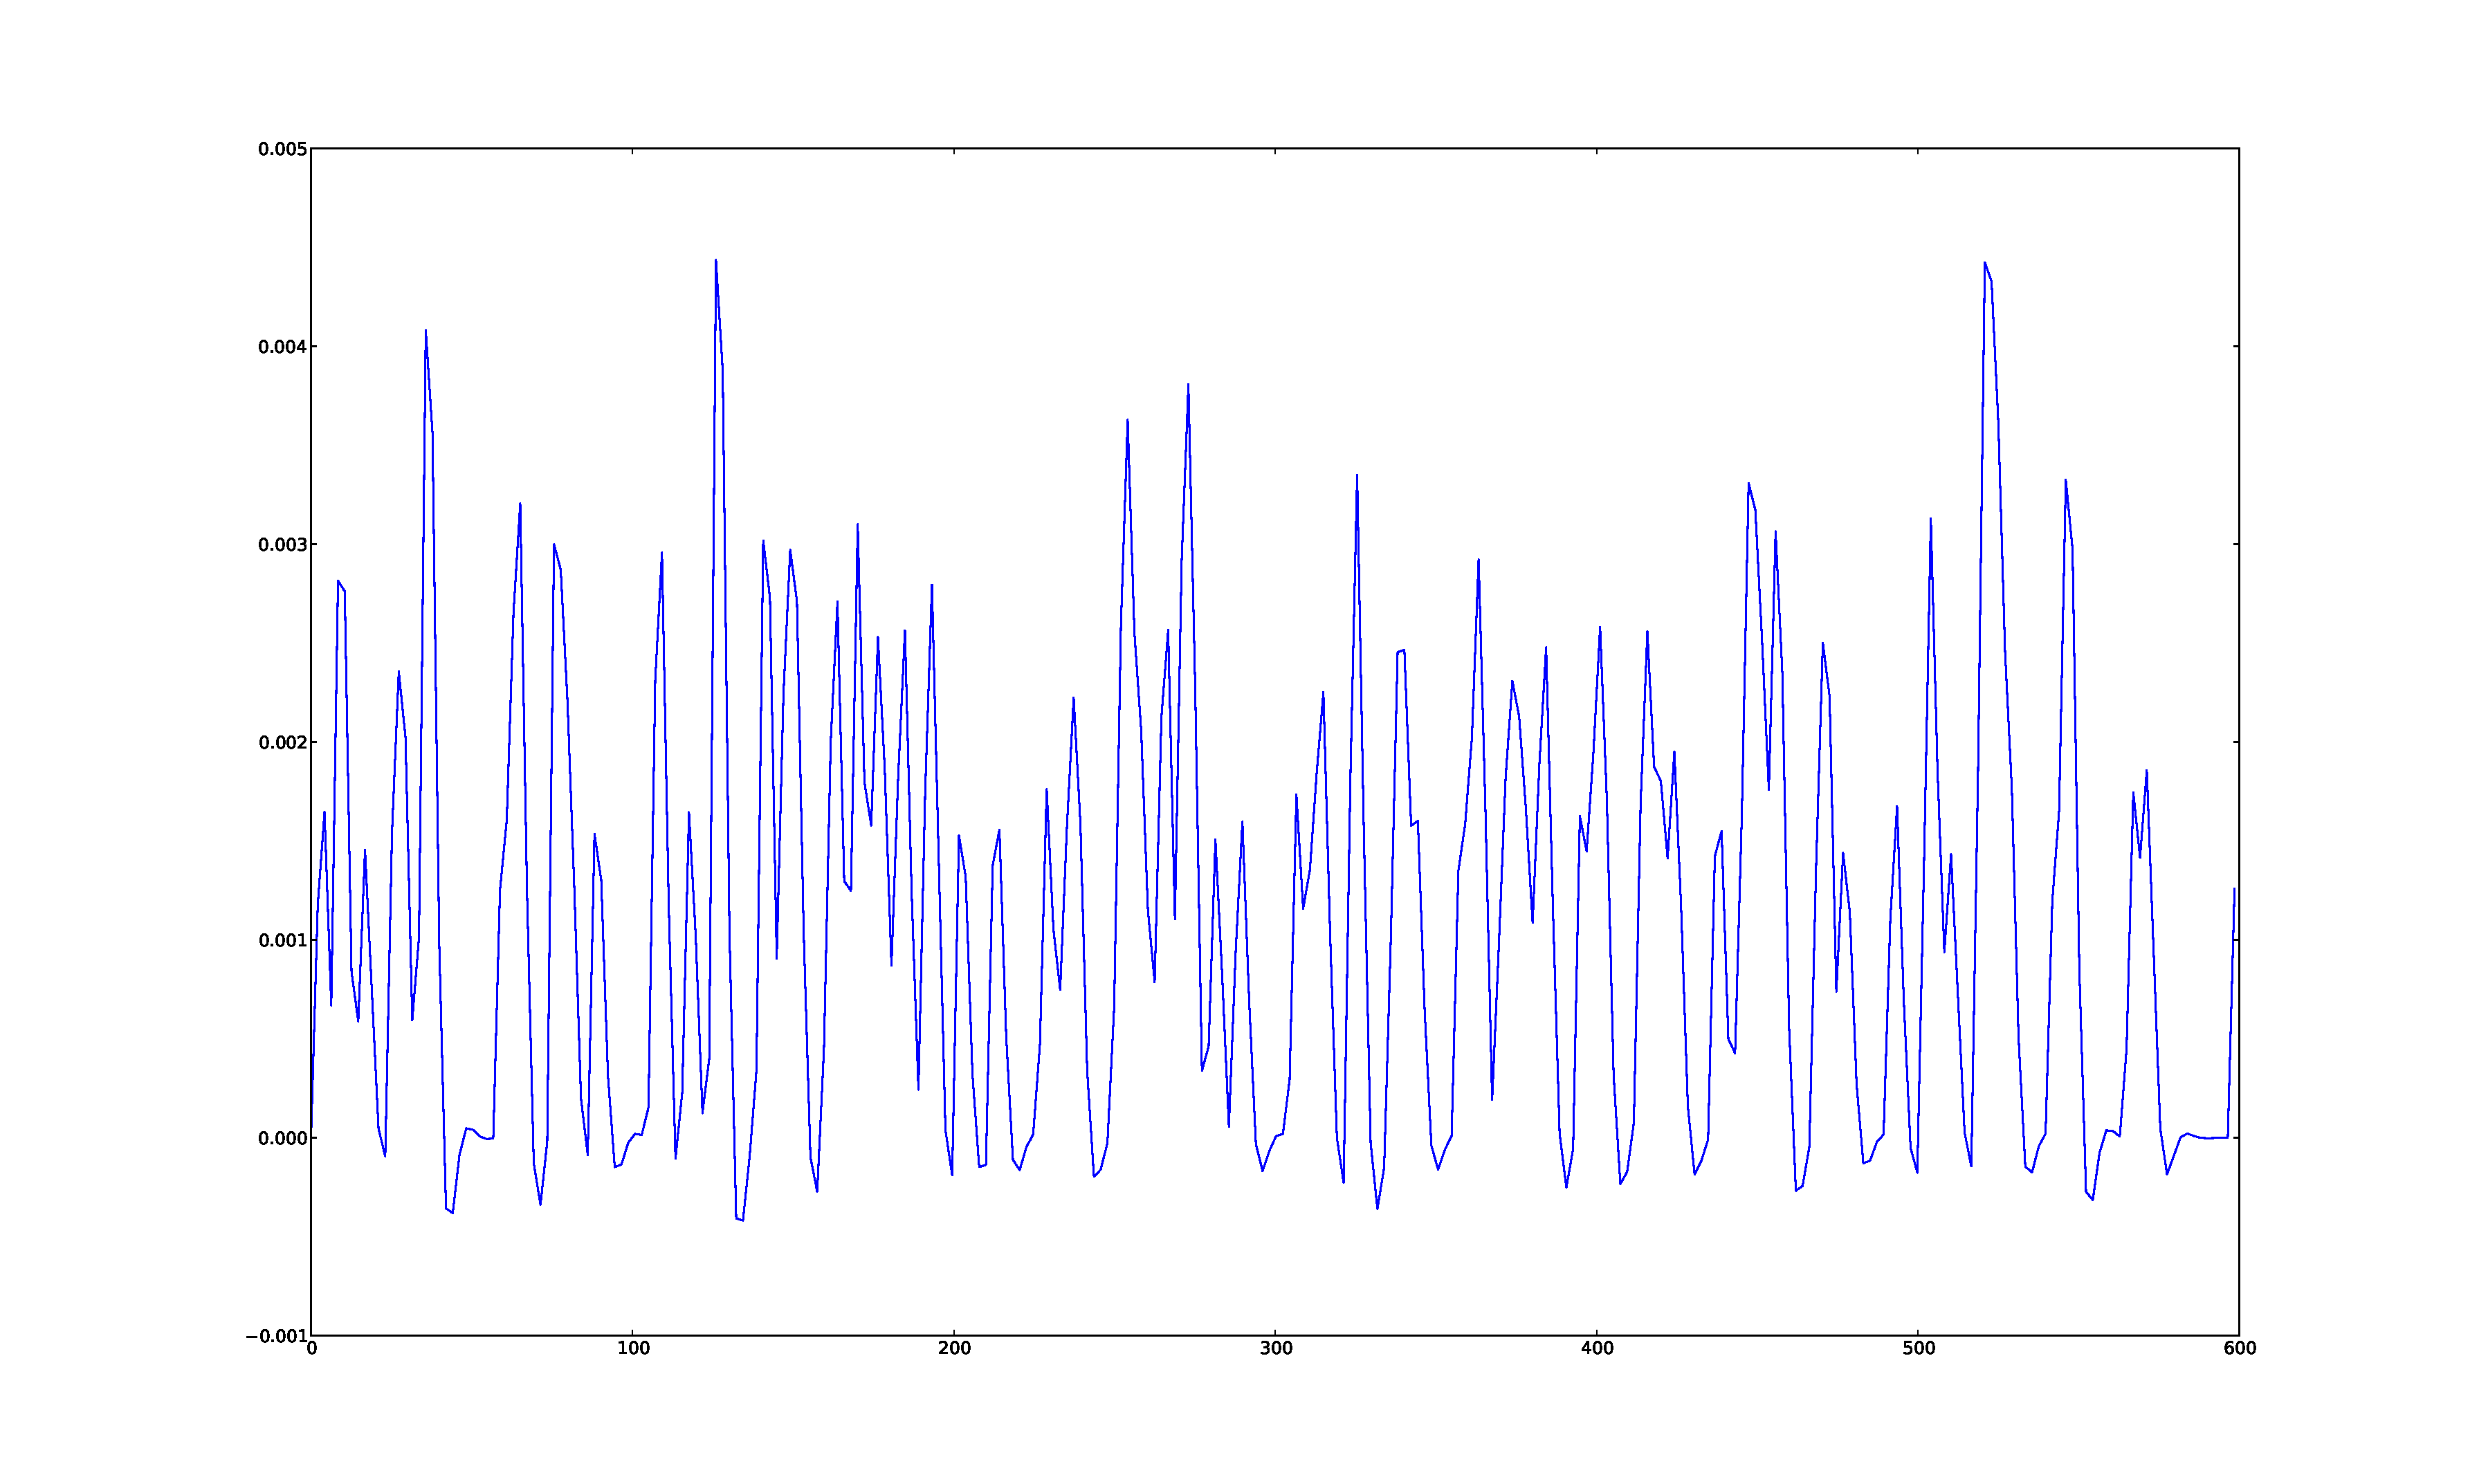
\includegraphics[clip=true,trim=6cm 3cm 6cm 3cm,height=9cm]{images/fits_noiseonly}
\caption[Results for non-active, low noise signal]  ($\sigma_x = 0.005$, $\sigma_y = 0.01$)
{Comparison of the estimated BOLD signal for the low noise signal-free case.
 ($\sigma_x = 0.005$, $\sigma_y = 0.01$). Note the line thickness is caused
by all the estimates overlapping.}
\label{fig:fits_noiseonly}
\end{figure}

\begin{table}[t]
\centering
\begin{tabular}{|c | c | c | c | c | c | c | c | c |}
\hline
$\tau_0$ & $\alpha$ & $E_0$    & $V_0$    & $\tau_s$ & $\tau_f$ & $\epsilon$  & \acs{RMSR} \\
\hline
1.0324 & 0.33211 & 0.34058 & 0.03012 & 1.40665 & 2.52079 & 0.5311 &   0.00167  \\
 0.98189 & 0.33047 & 0.3386 & 0.03014 & 1.45707 & 2.47232 & 0.45049 & 0.00159   \\
 1.0429 & 0.33224 & 0.34124 & 0.02946 & 1.4618 & 2.49245 & 0.43012 &  0.00165   \\
 1.02054 & 0.3321 & 0.33484 & 0.02586 & 1.45848 & 2.48741 & 0.4193 &  0.00151   \\
 1.0565 & 0.33405 & 0.33758 & 0.02791 & 1.43784 & 2.52545 & 0.47517 & 0.00152   \\
 1.01867 & 0.33528 & 0.33918 & 0.02782 & 1.48345 & 2.49605 & 0.44209 &0.00156   \\
 1.051 & 0.33038 & 0.33837 & 0.02985 & 1.47651 & 2.48621 & 0.42719 &  0.00159   \\
 1.00281 & 0.32929 & 0.33988 & 0.0298 & 1.43519 & 2.49256 & 0.48899 & 0.00164   \\
 1.00893 & 0.33273 & 0.33982 & 0.0289 & 1.42903 & 2.49754 & 0.45688 & 0.00168   \\
 1.01289 & 0.33275 & 0.3376 & 0.02997 & 1.41188 & 2.49881 & 0.50628 & 0.00183   \\
 1.10247 & 0.33371 & 0.3419 & 0.02939 & 1.43774 & 2.53384 & 0.44079 & 0.00195   \\
\hline
1.03009 & 0.33228 & 0.33905 & 0.02902 & 1.44506 & 2.50031 & 0.46076 & 0.00165 \\
\hline
\end{tabular}
\caption{Estimated Parameters on 11 different runs with low noise and no signal present.
 ($\sigma_x = 0.005$, $\sigma_y = 0.01$)}
\label{tab:NoiseOnlyResults}
\end{table}

\begin{figure}[H]
\centering
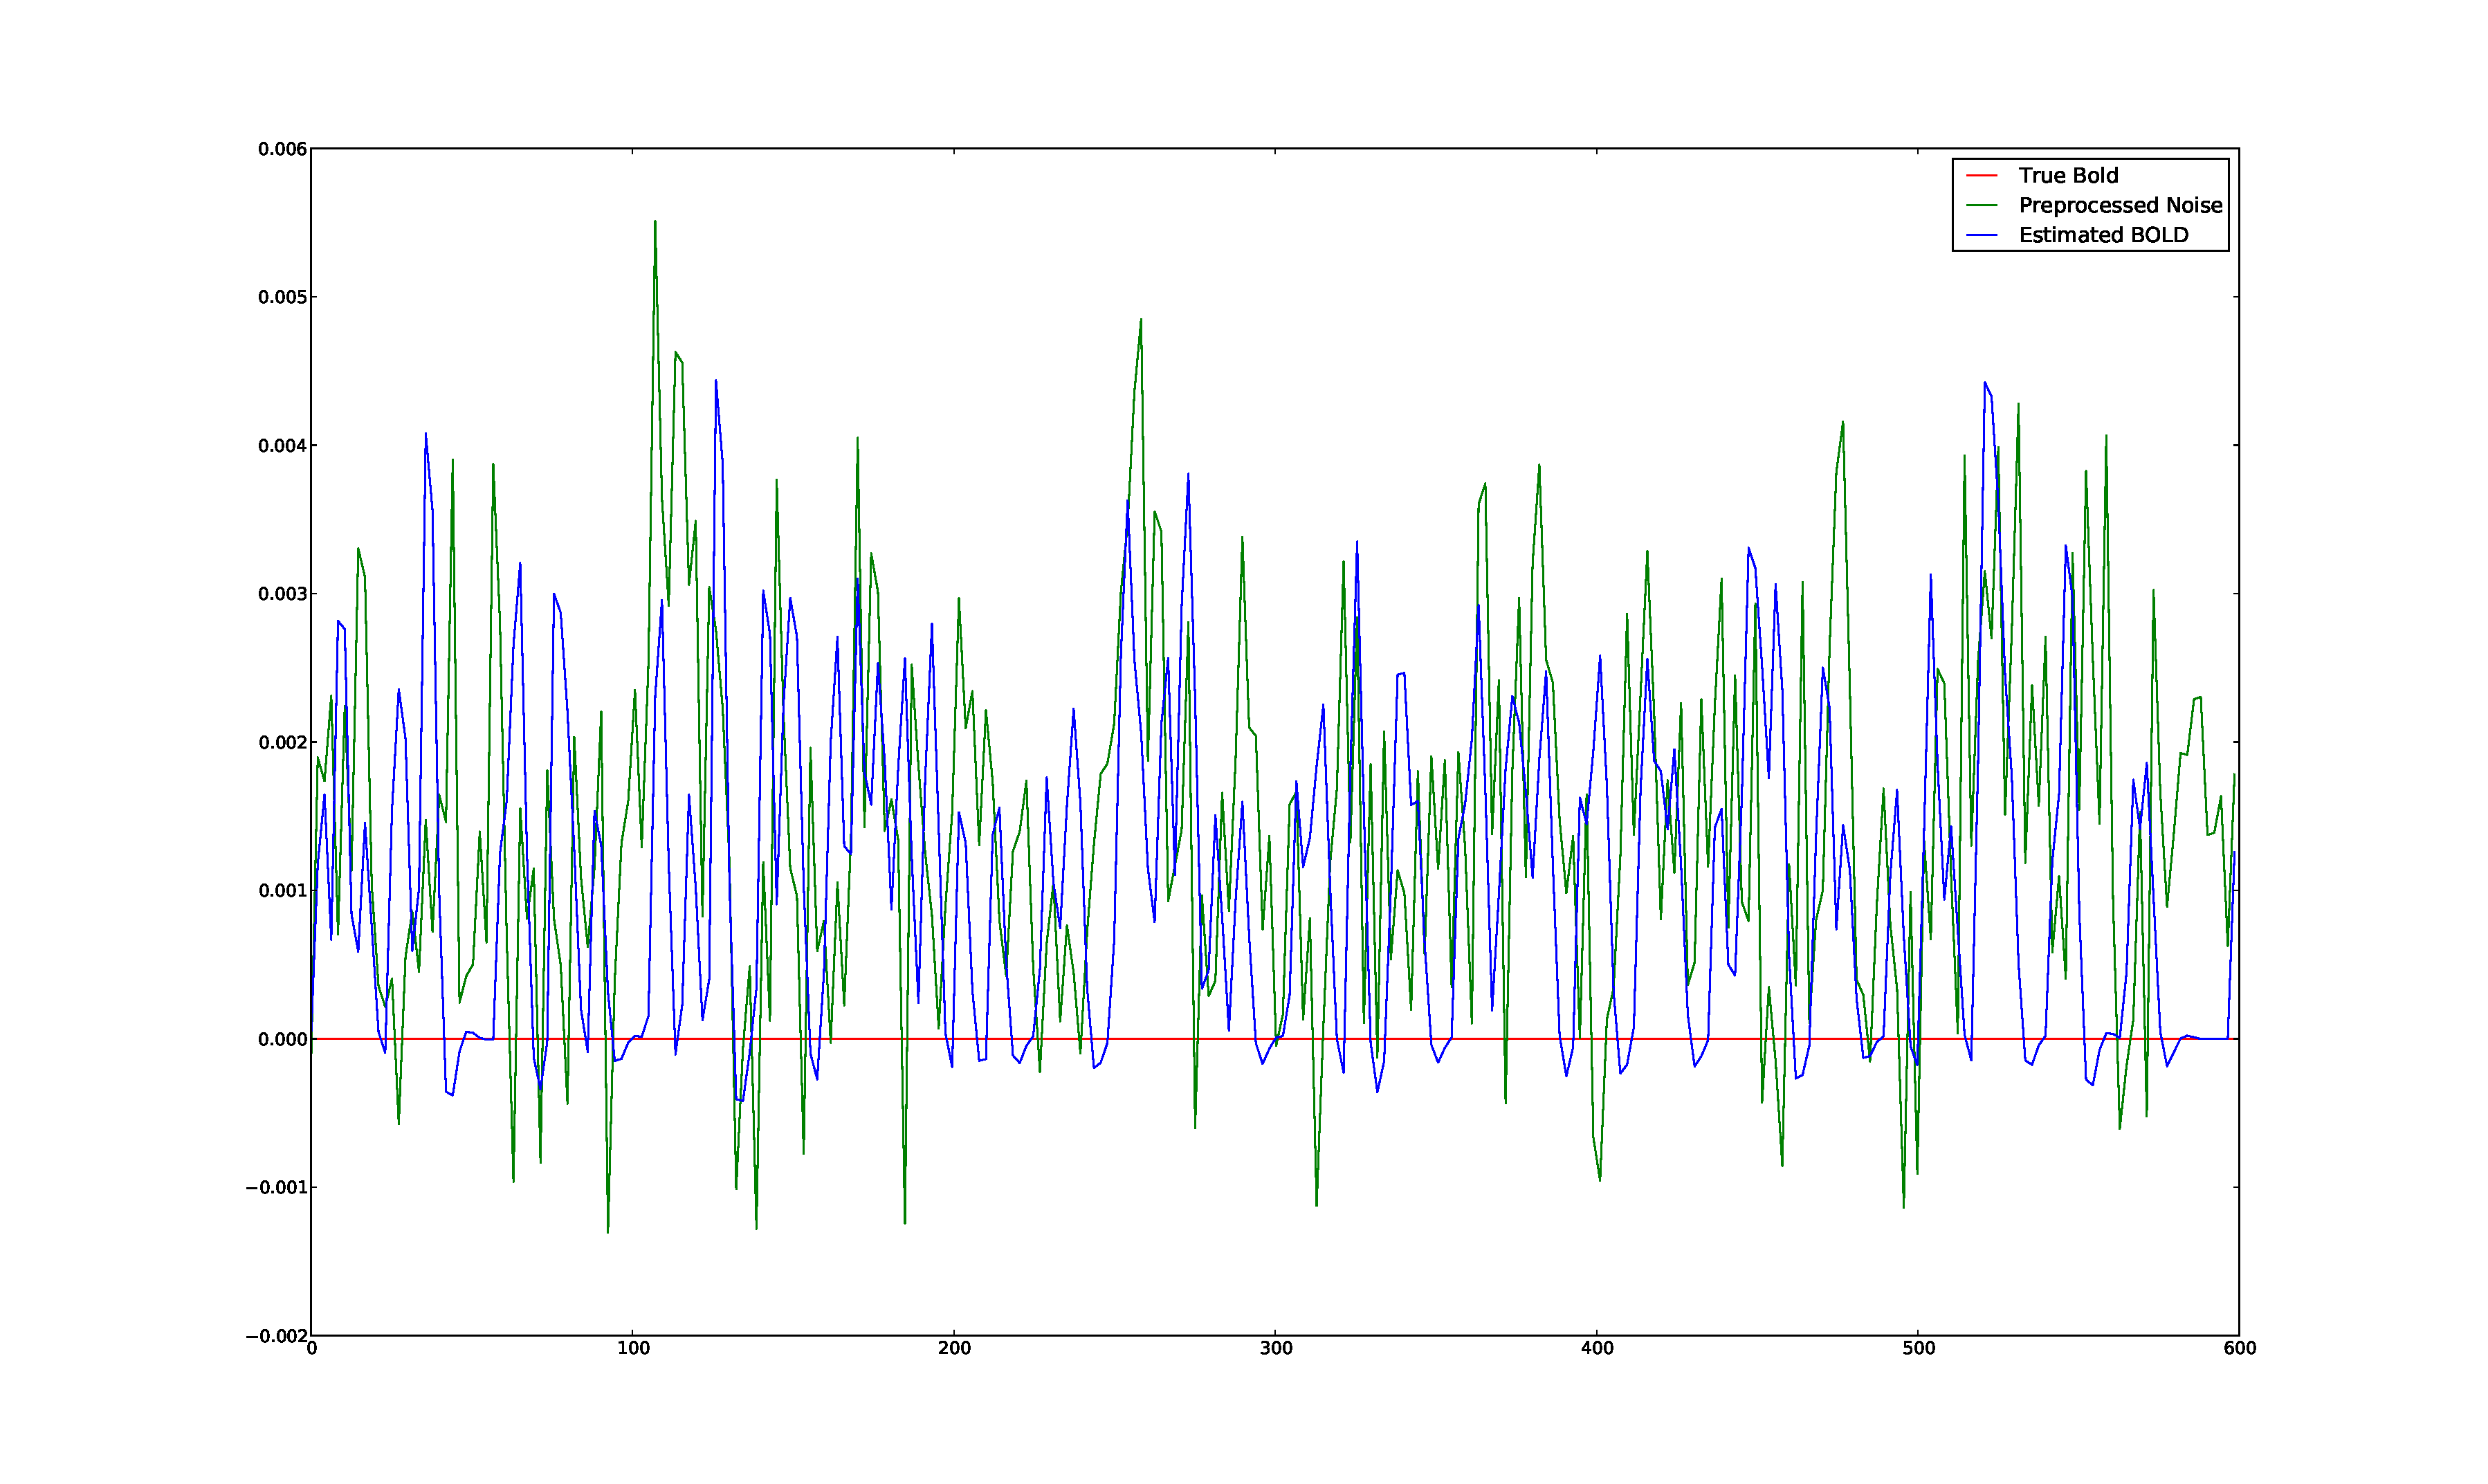
\includegraphics[clip=true,trim=6cm 3cm 6cm 3cm,height=9cm]{images/justnoise_fit_0}
\caption{Single Fit Results for non-active, low noise signal.}
\label{fig:justnoise_fit_0}
\end{figure} %uses allnoise/ALLNOISE-0-w0

\begin{figure}[H]
\centering
\subfigure
{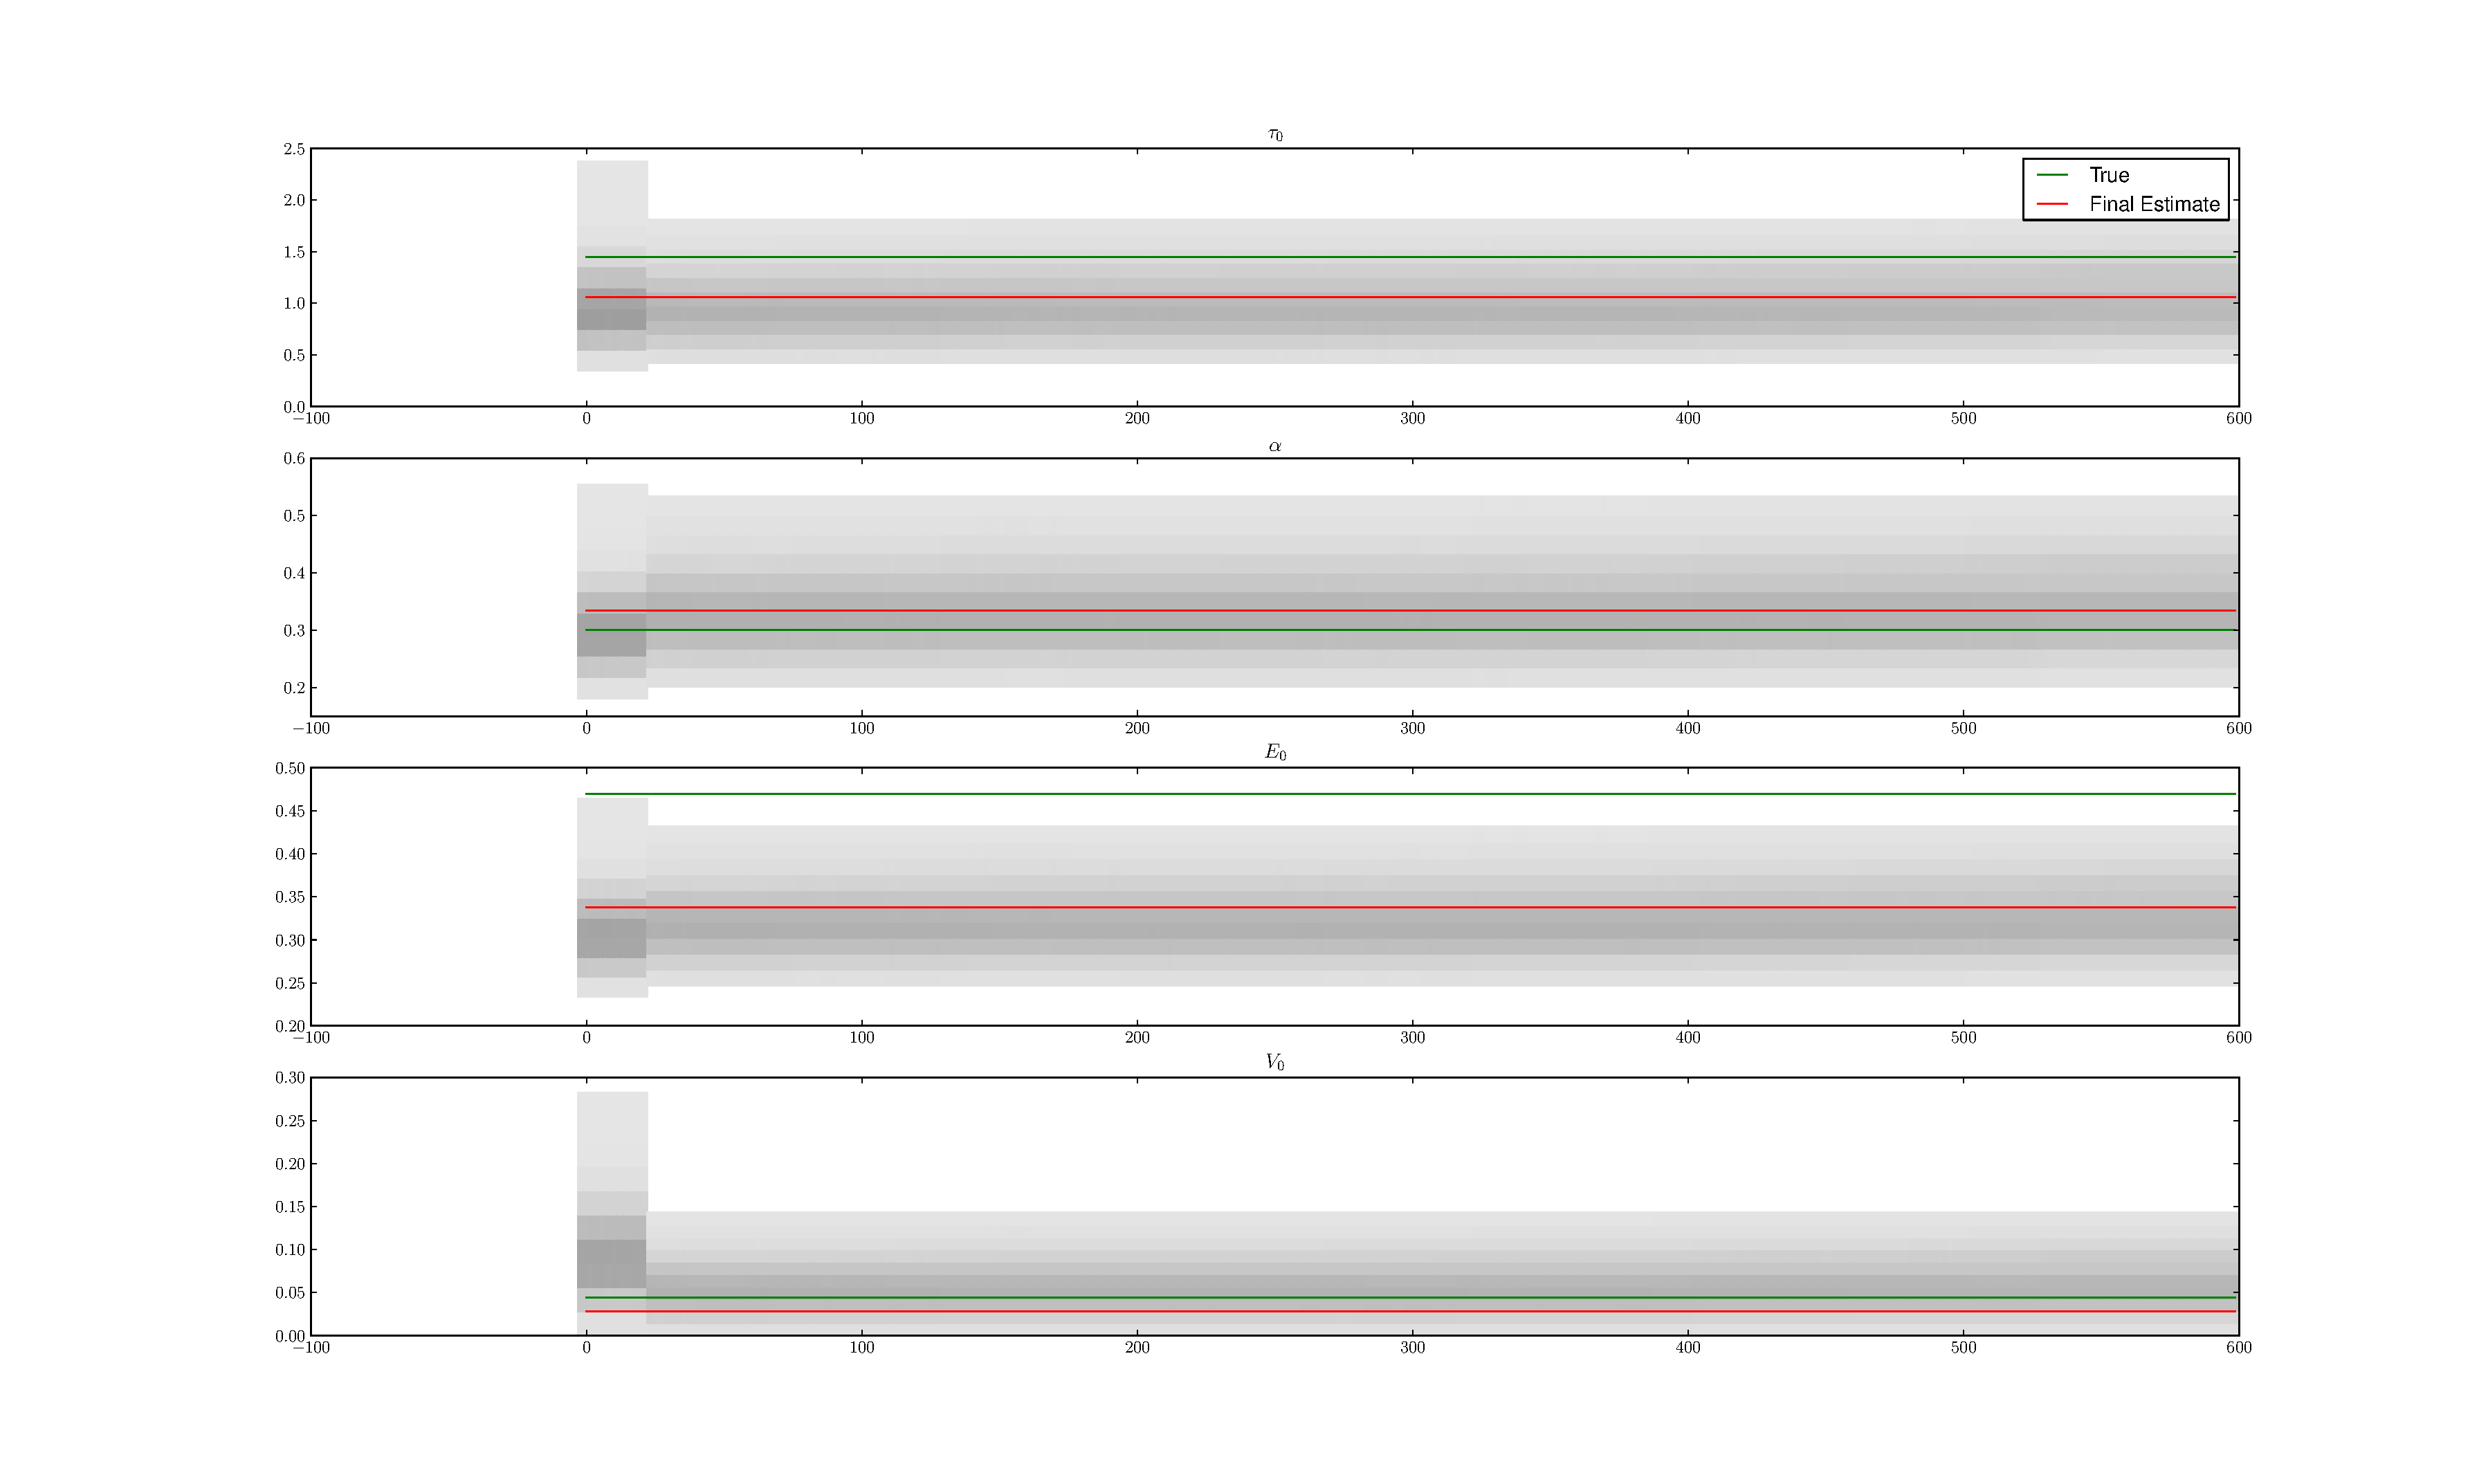
\includegraphics[clip=true,trim=7cm 3cm 6cm 3cm, width=\textwidth]{images/justnoise_hist_1}}
\subfigure
{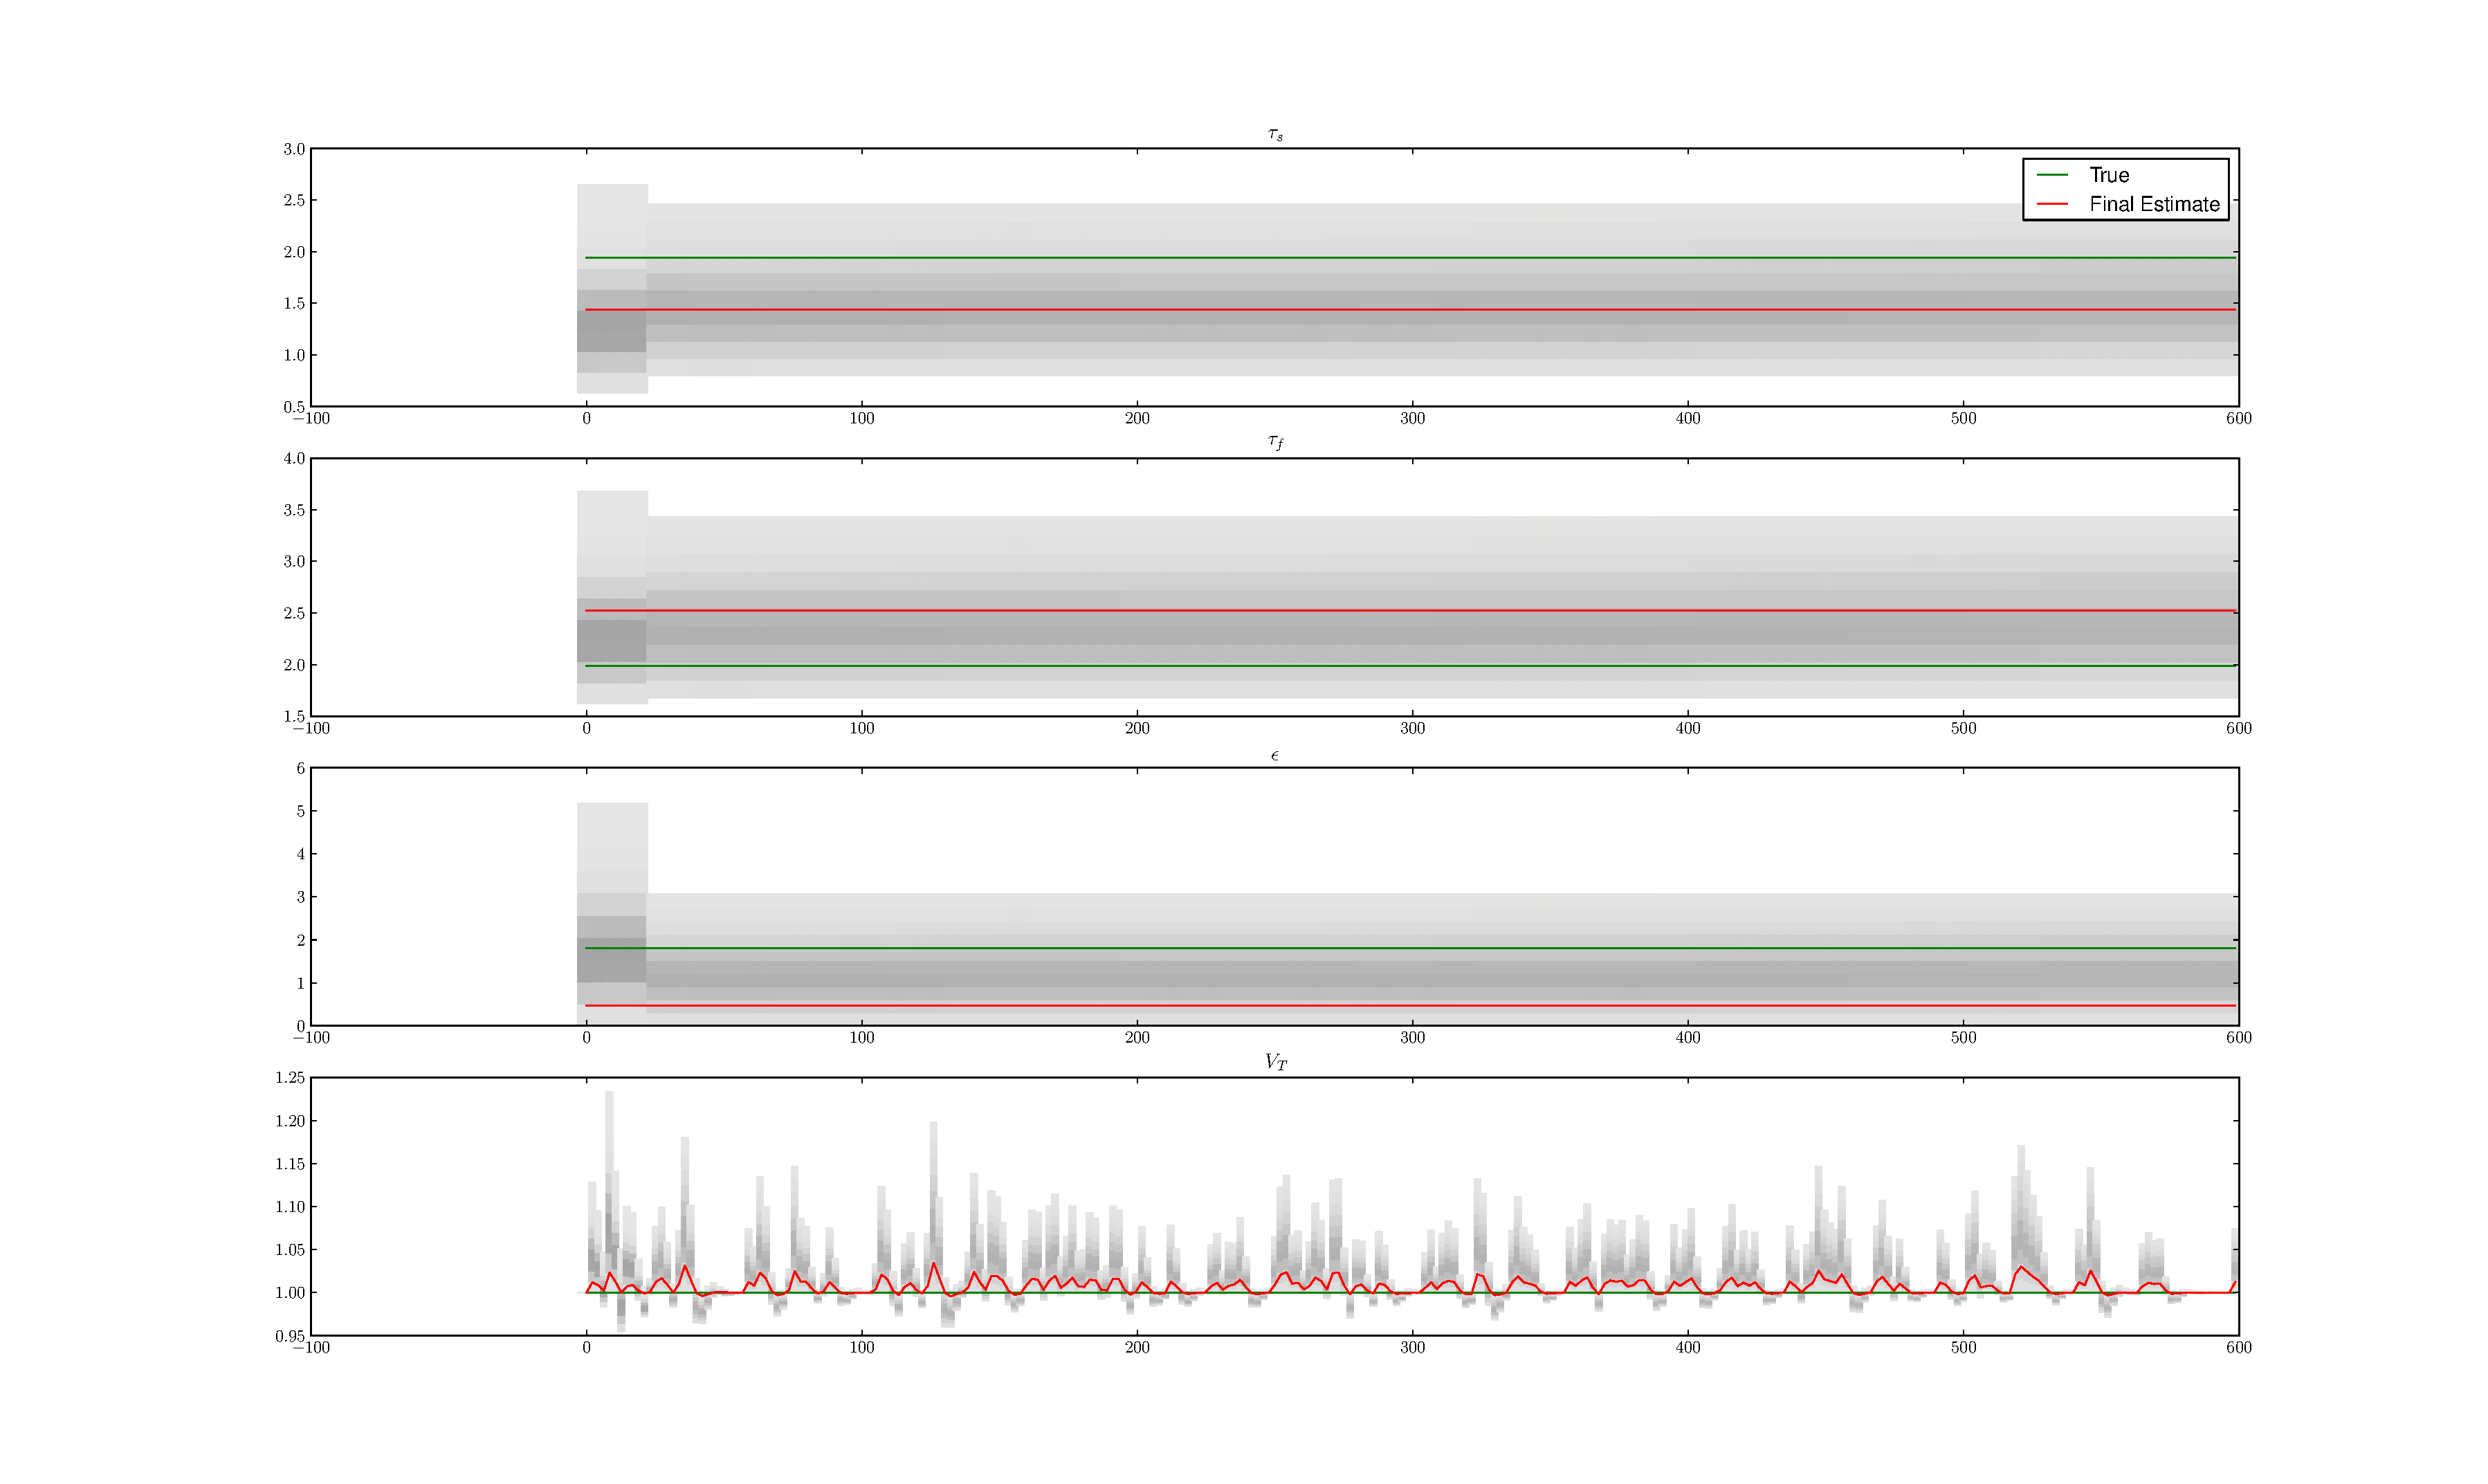
\includegraphics[clip=true,trim=7cm 3cm 6cm 3cm, width=\textwidth]{images/justnoise_hist_2}}
\end{figure}

\begin{figure}[H]
\centering
\subfigure
{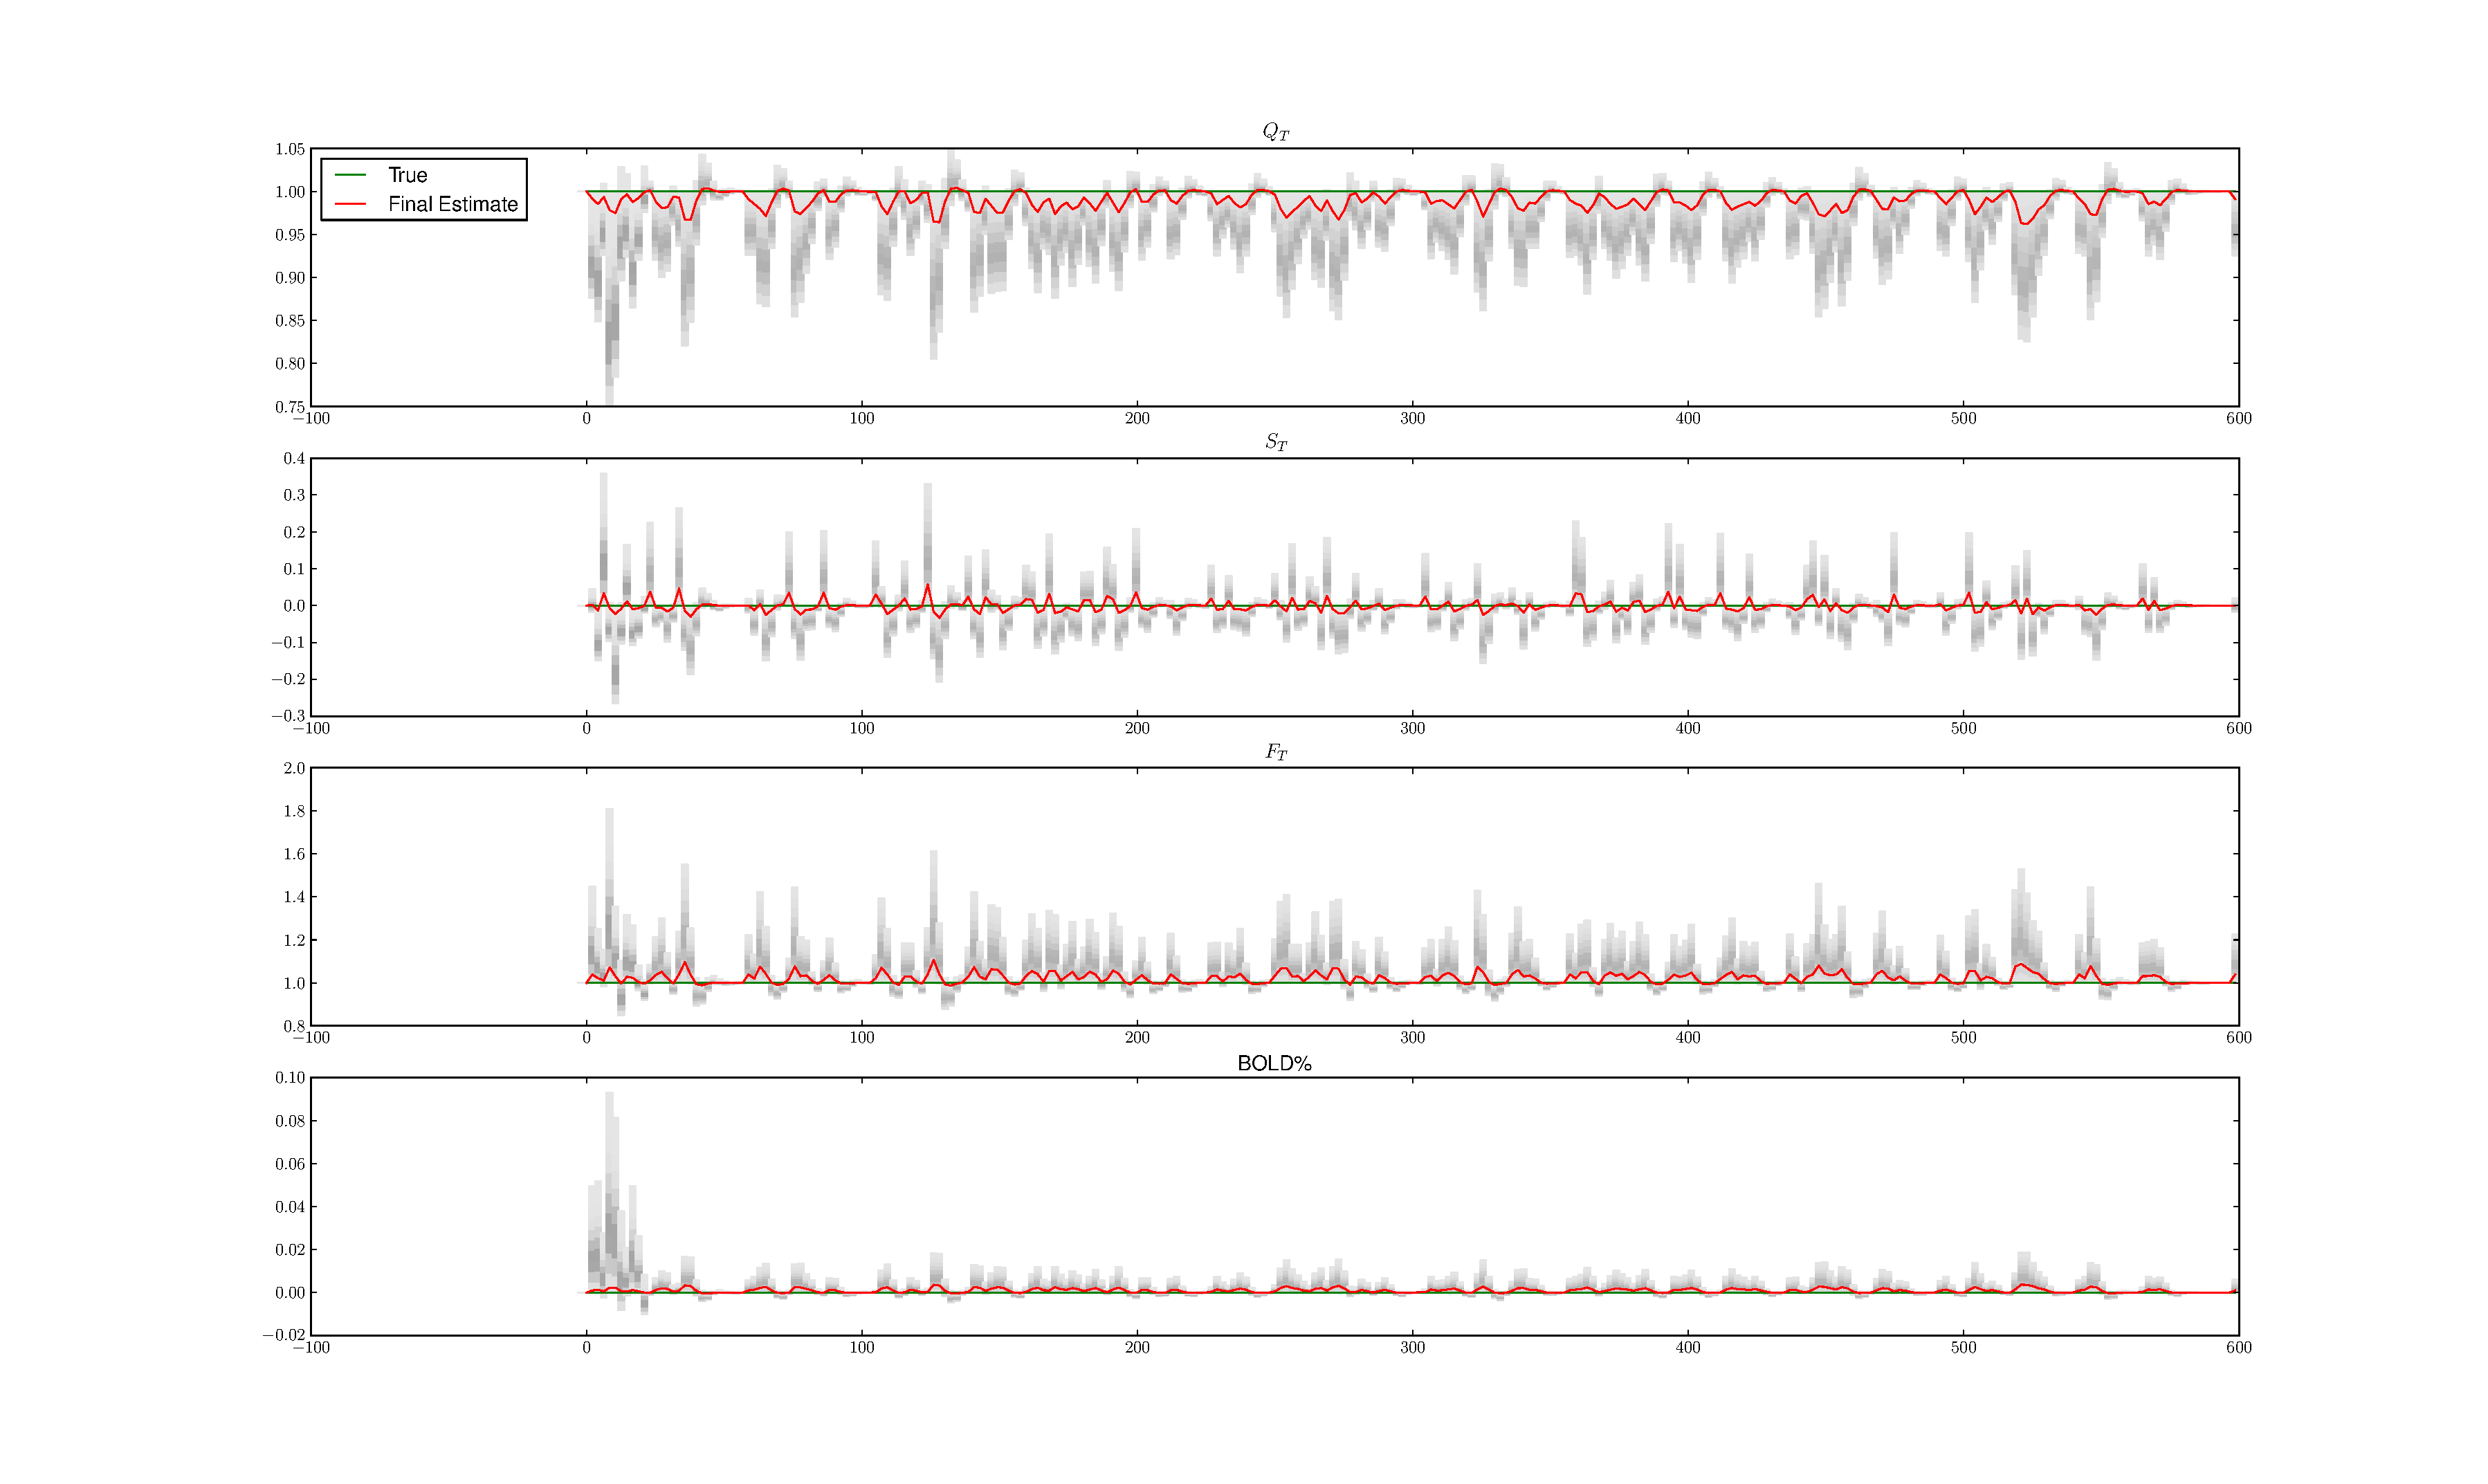
\includegraphics[clip=true,trim=7cm 3cm 6cm 3cm, width=\textwidth]{images/justnoise_hist_3}}
\caption[Convergence of the parameters during a noise-only run.]
{Convergence of the parameters when the signal consisted purely of low level noise 
($\sigma_x = 0.01$, $\sigma_y = 0.005$).
Order of estimates: $\tau_0, \alpha, E_0, V_0, \tau_s, \tau_f, \epsilon, v,
q, s, f, BOLD$.  The bars represent
a histogram, where darker bars indicate more particles with parameters in that bin. The red 
line is the parameter used to generate the true signal, blue line is the final mean of the
particles. See \autoref{fig:justnoise_fit_0}}
\label{fig:JustNoiseConvergence}
\end{figure}

The data shows that the parameters did not converge
(\autoref{fig:JustNoiseConvergence}).
The peaks never even reached 1\% difference
(\autoref{fig:PreprocessedNoiseOnly}) so  the signal  stayed
well within the range of $0.005$, the standard deviation of the weighting function.
Note that the \acp{RMSR}
were actually lower than the \acp{RMSR} in the low noise simulation 
from \autoref{sec:SimLowNoise}
and the parameter estimates were more consistent across 11 runs.
The low \ac{RMSR} was caused by the overall
signal being significantly smaller than any previous simulation.
This run would benefit greatly from an adaptive weight function, since
such a much tighter weighting function would have forced the particle
filter to fail.

%NO SIGNAL, VERY HIGH NOISE
\subsection{Pure Noise, High Magnitude}
\label{sec:PureNoiseHighMag}
To determine how the particle filter responds to active, yet unrelated
portions of the brain, this section repeats the test of \autoref{sec:PureNoiseLowMag}
with much higher noise peaks. To simulate this case another
pure noise signal was generated using $\sigma_x$ of $0.1$ and $\sigma_y$ of $0.05$.

As before, the convergence all follows a similar path, leaving almost no
variance in the estimated time series (\autoref{fig:fits_noiseonly_high}).
Interestingly the algorithm suffered from almost constant particle deprivation,
meaning that the heuristic
for rescuing the particle filter from particle deprivation, discussed in
\autoref{sec:Particle Deprivation} was used when it shouldn't have been.
 When this mechanism
was removed, all 11 runs stopped due to particle deprivation (all weights hit zero).
The problem with allowing particle deprivation to occur is that it can \emph{rarely}
occur in otherwise good data if resampling is performed at the wrong moment.

Because of the preprocessing steps, the pure noise signal can look markedly like a real
signal (\autoref{fig:justbignoise_fit_0}). The preprocessing causes the particle filter
to converge to a non-zero response in spite of the fact that the input does not correlate
with the stimuli in any way (\autoref{fig:fits_noiseonly_high}).

\begin{figure}[H]
\centering
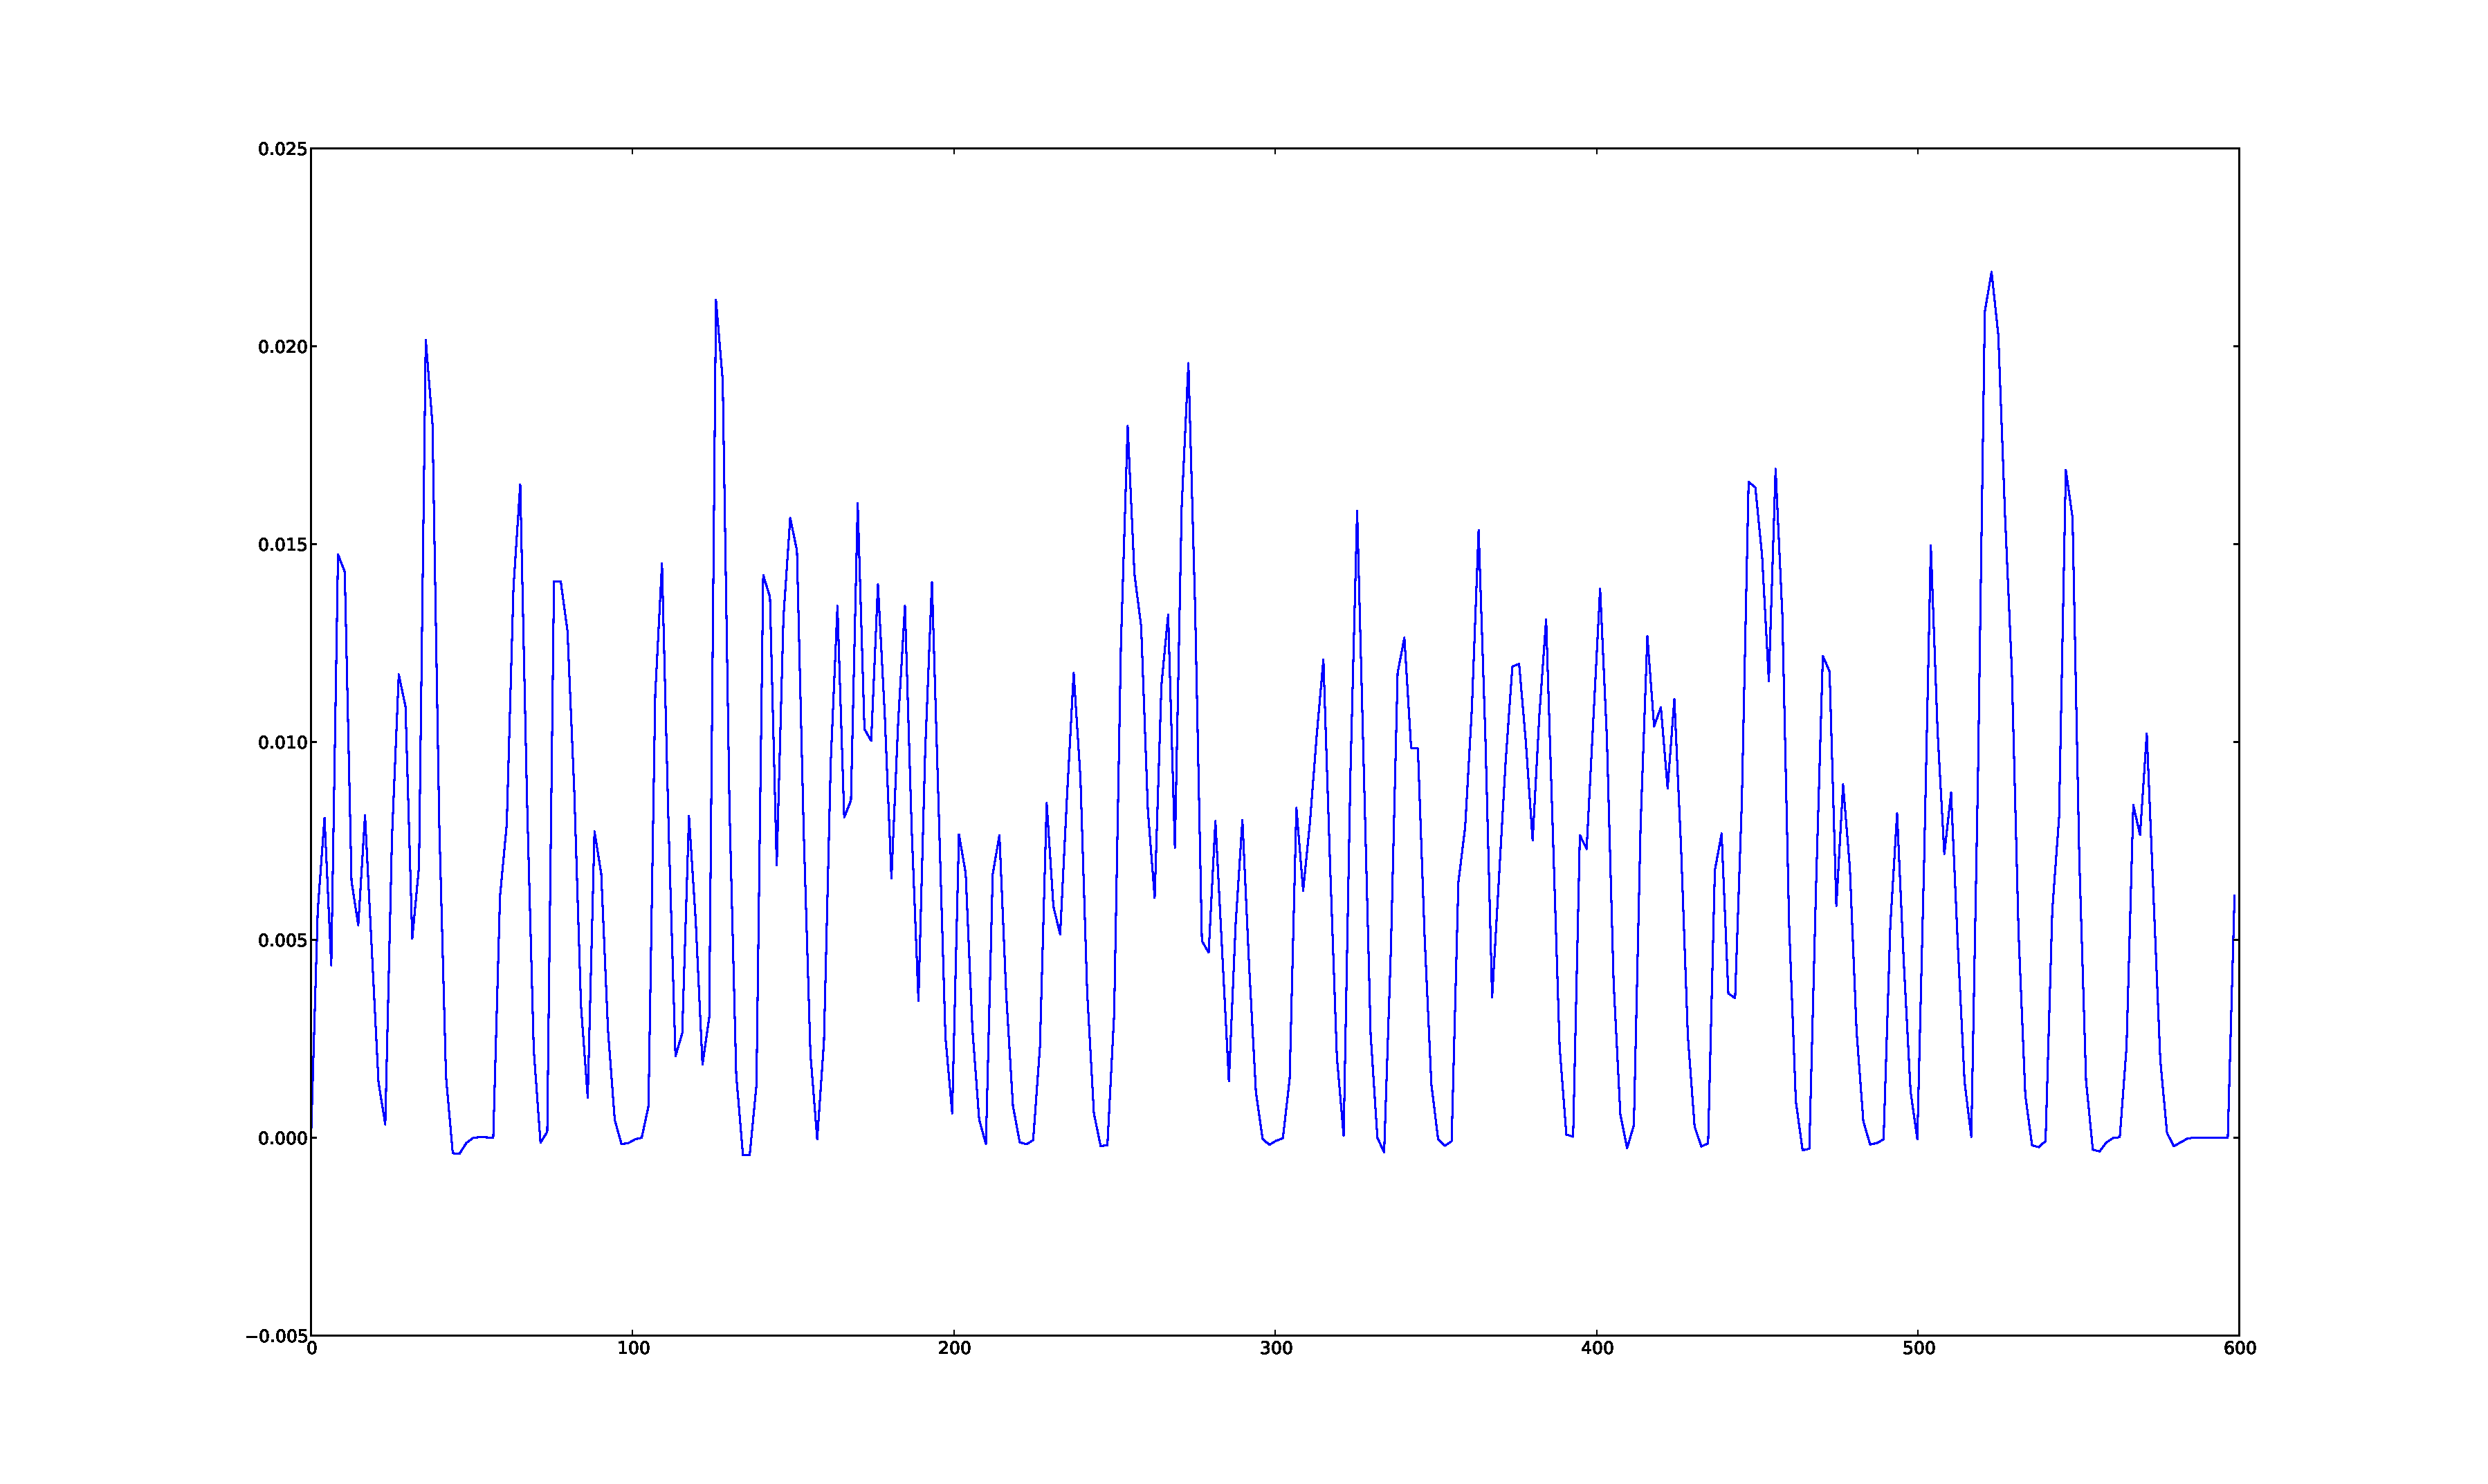
\includegraphics[clip=true,trim=6cm 2cm 5cm 3cm,width=15cm]{images/fits_noiseonly_high}
\caption[Results for non-active, high noise signal.]
{\ac{BOLD} estimates for the non-active, high noise signal ($\sigma_x = 0.1$, $\sigma_y = 0.05$). 
Note the line thickness is caused by all the estimates overlapping.}
\label{fig:fits_noiseonly_high}
\end{figure}

\begin{figure}[H]
\centering
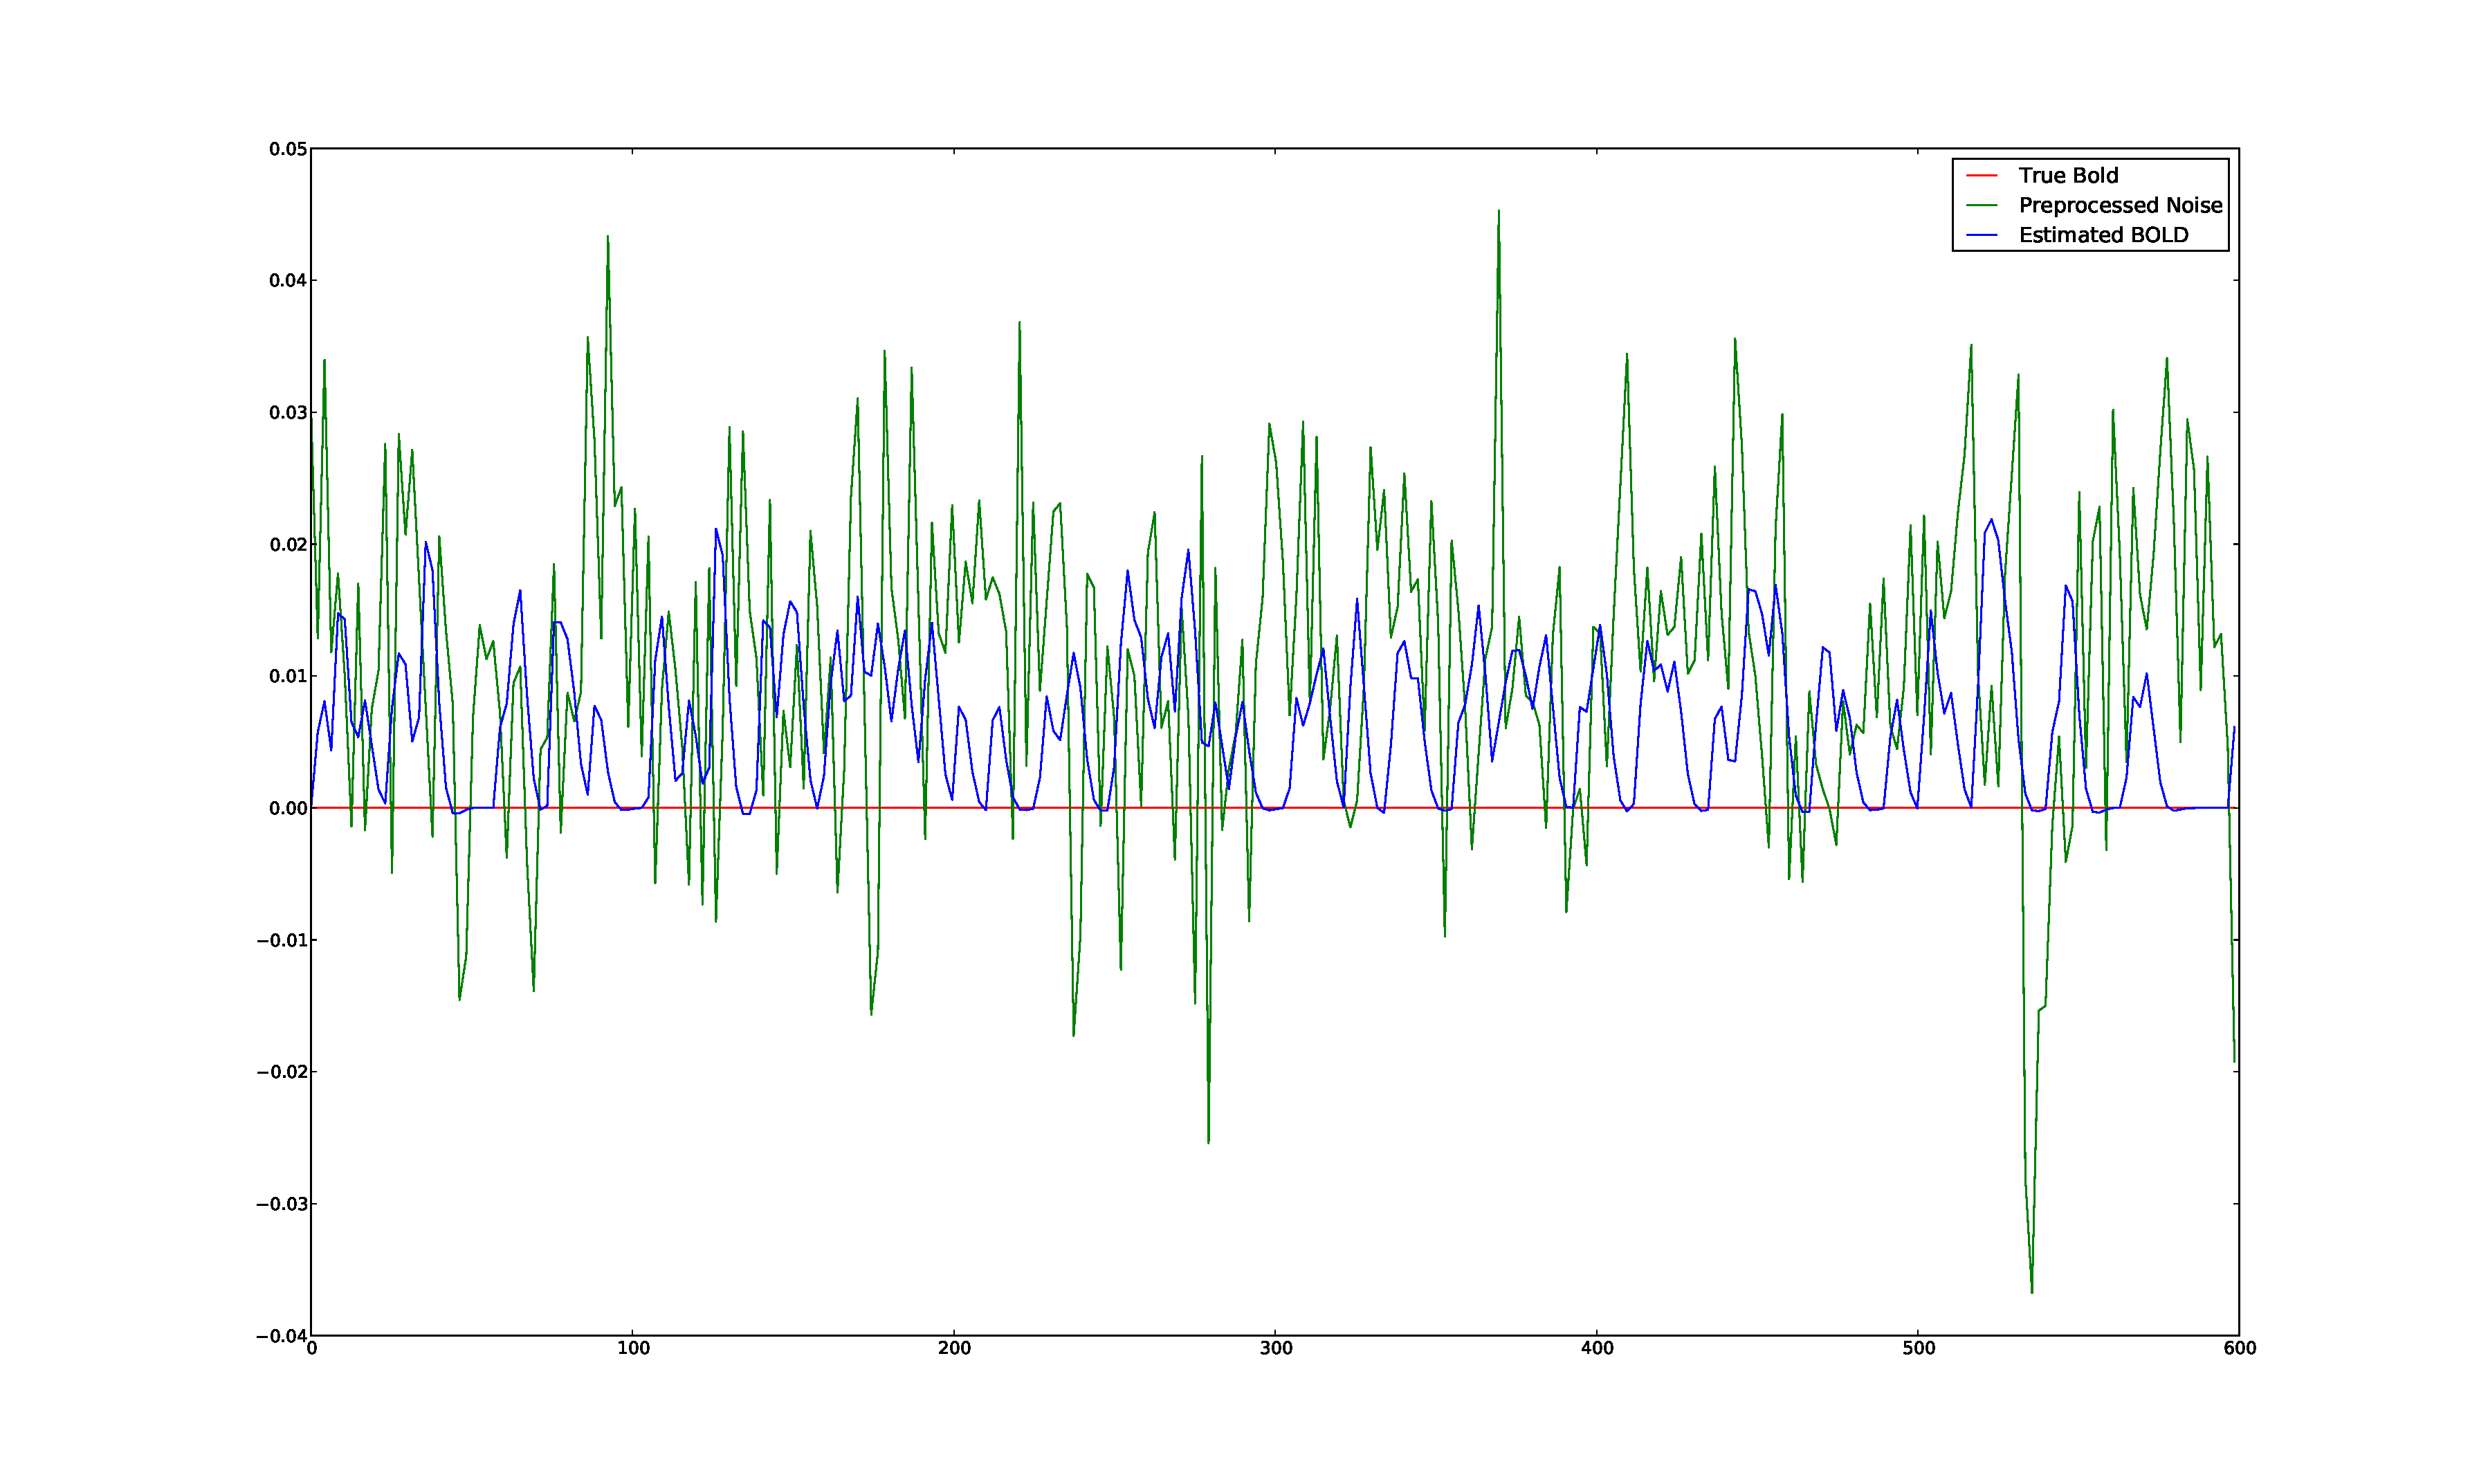
\includegraphics[clip=true,trim=6cm 3cm 6cm 3cm,height=9cm]{images/justbignoise_fit_0}
\caption{Single Fit Results for non-active, high noise signal.}
\label{fig:justbignoise_fit_0}
\end{figure} %uses allnoise/ALLNOISE-0-w0

%\begin{figure}[H]
%\centering
%\subfigure[$\tau_0$, $\alpha$, $E_0$, $V_0$]
%{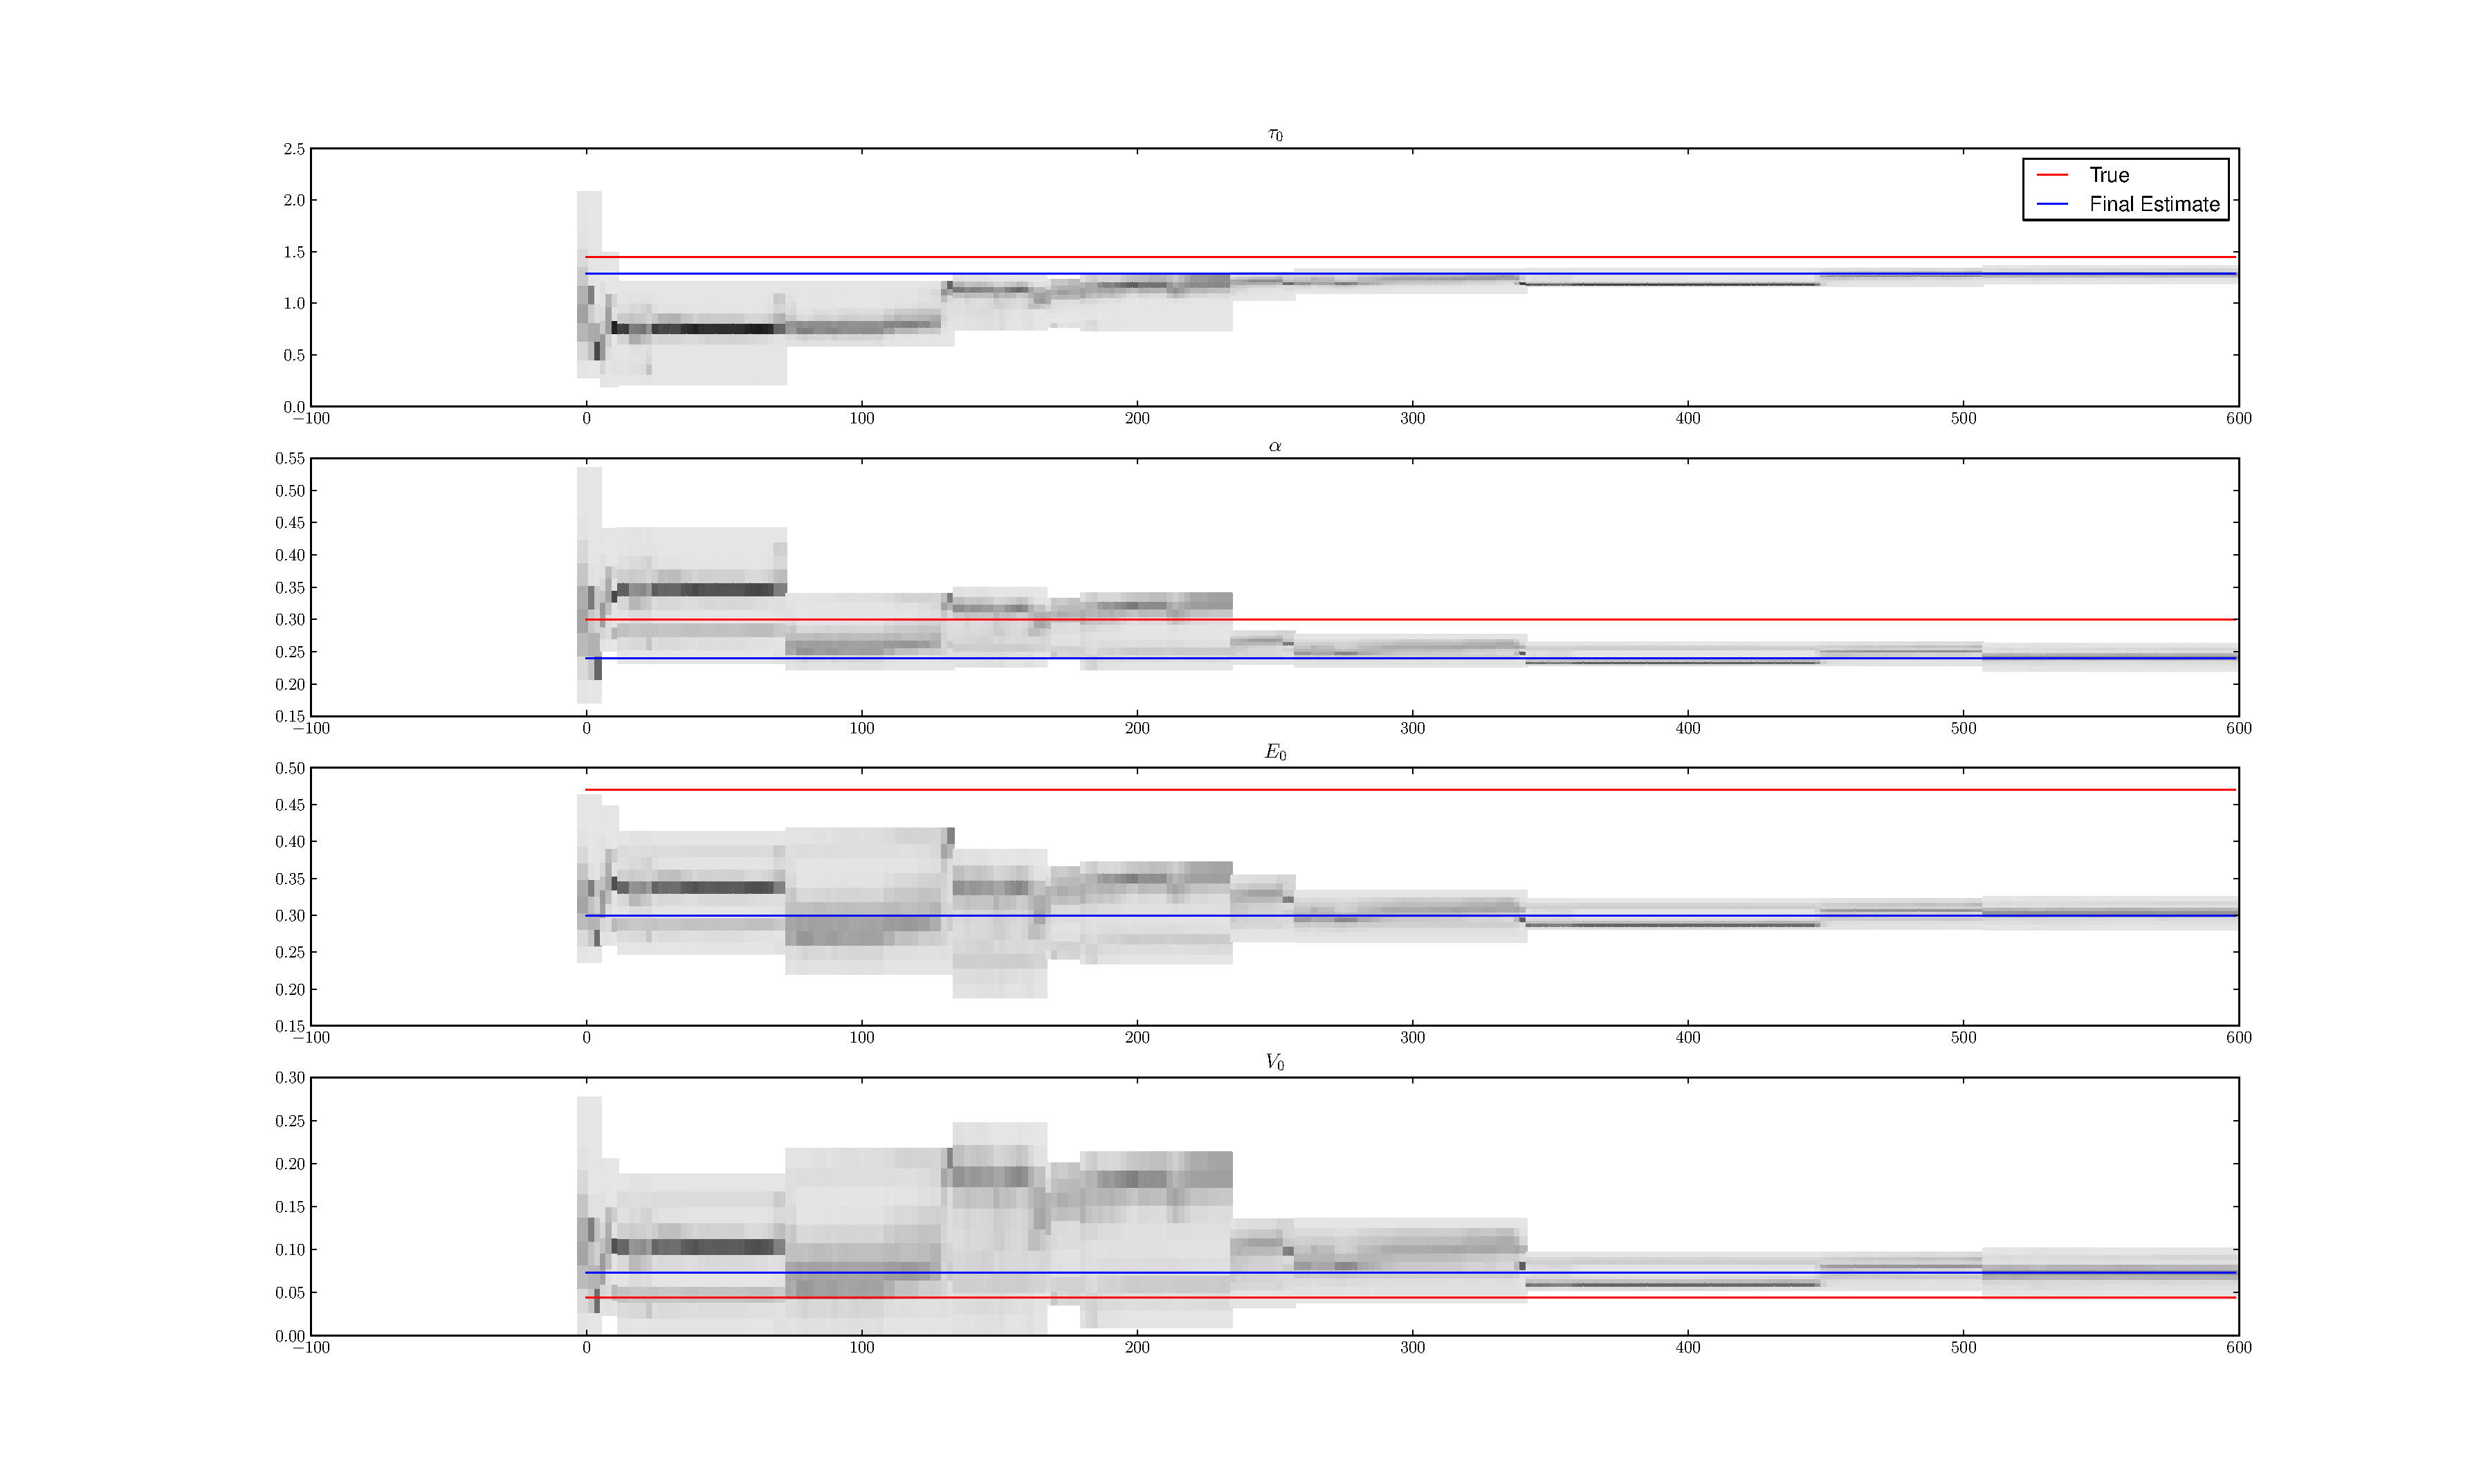
\includegraphics[clip=true,trim=6cm 3cm 6cm 3cm, height=9cm]{images/justbignoise_1}}\\
%\end{figure}
%\begin{figure}[H]
%\subfigure[$\tau_s$, $\tau_f$, $\epsilon$, $v$]
%{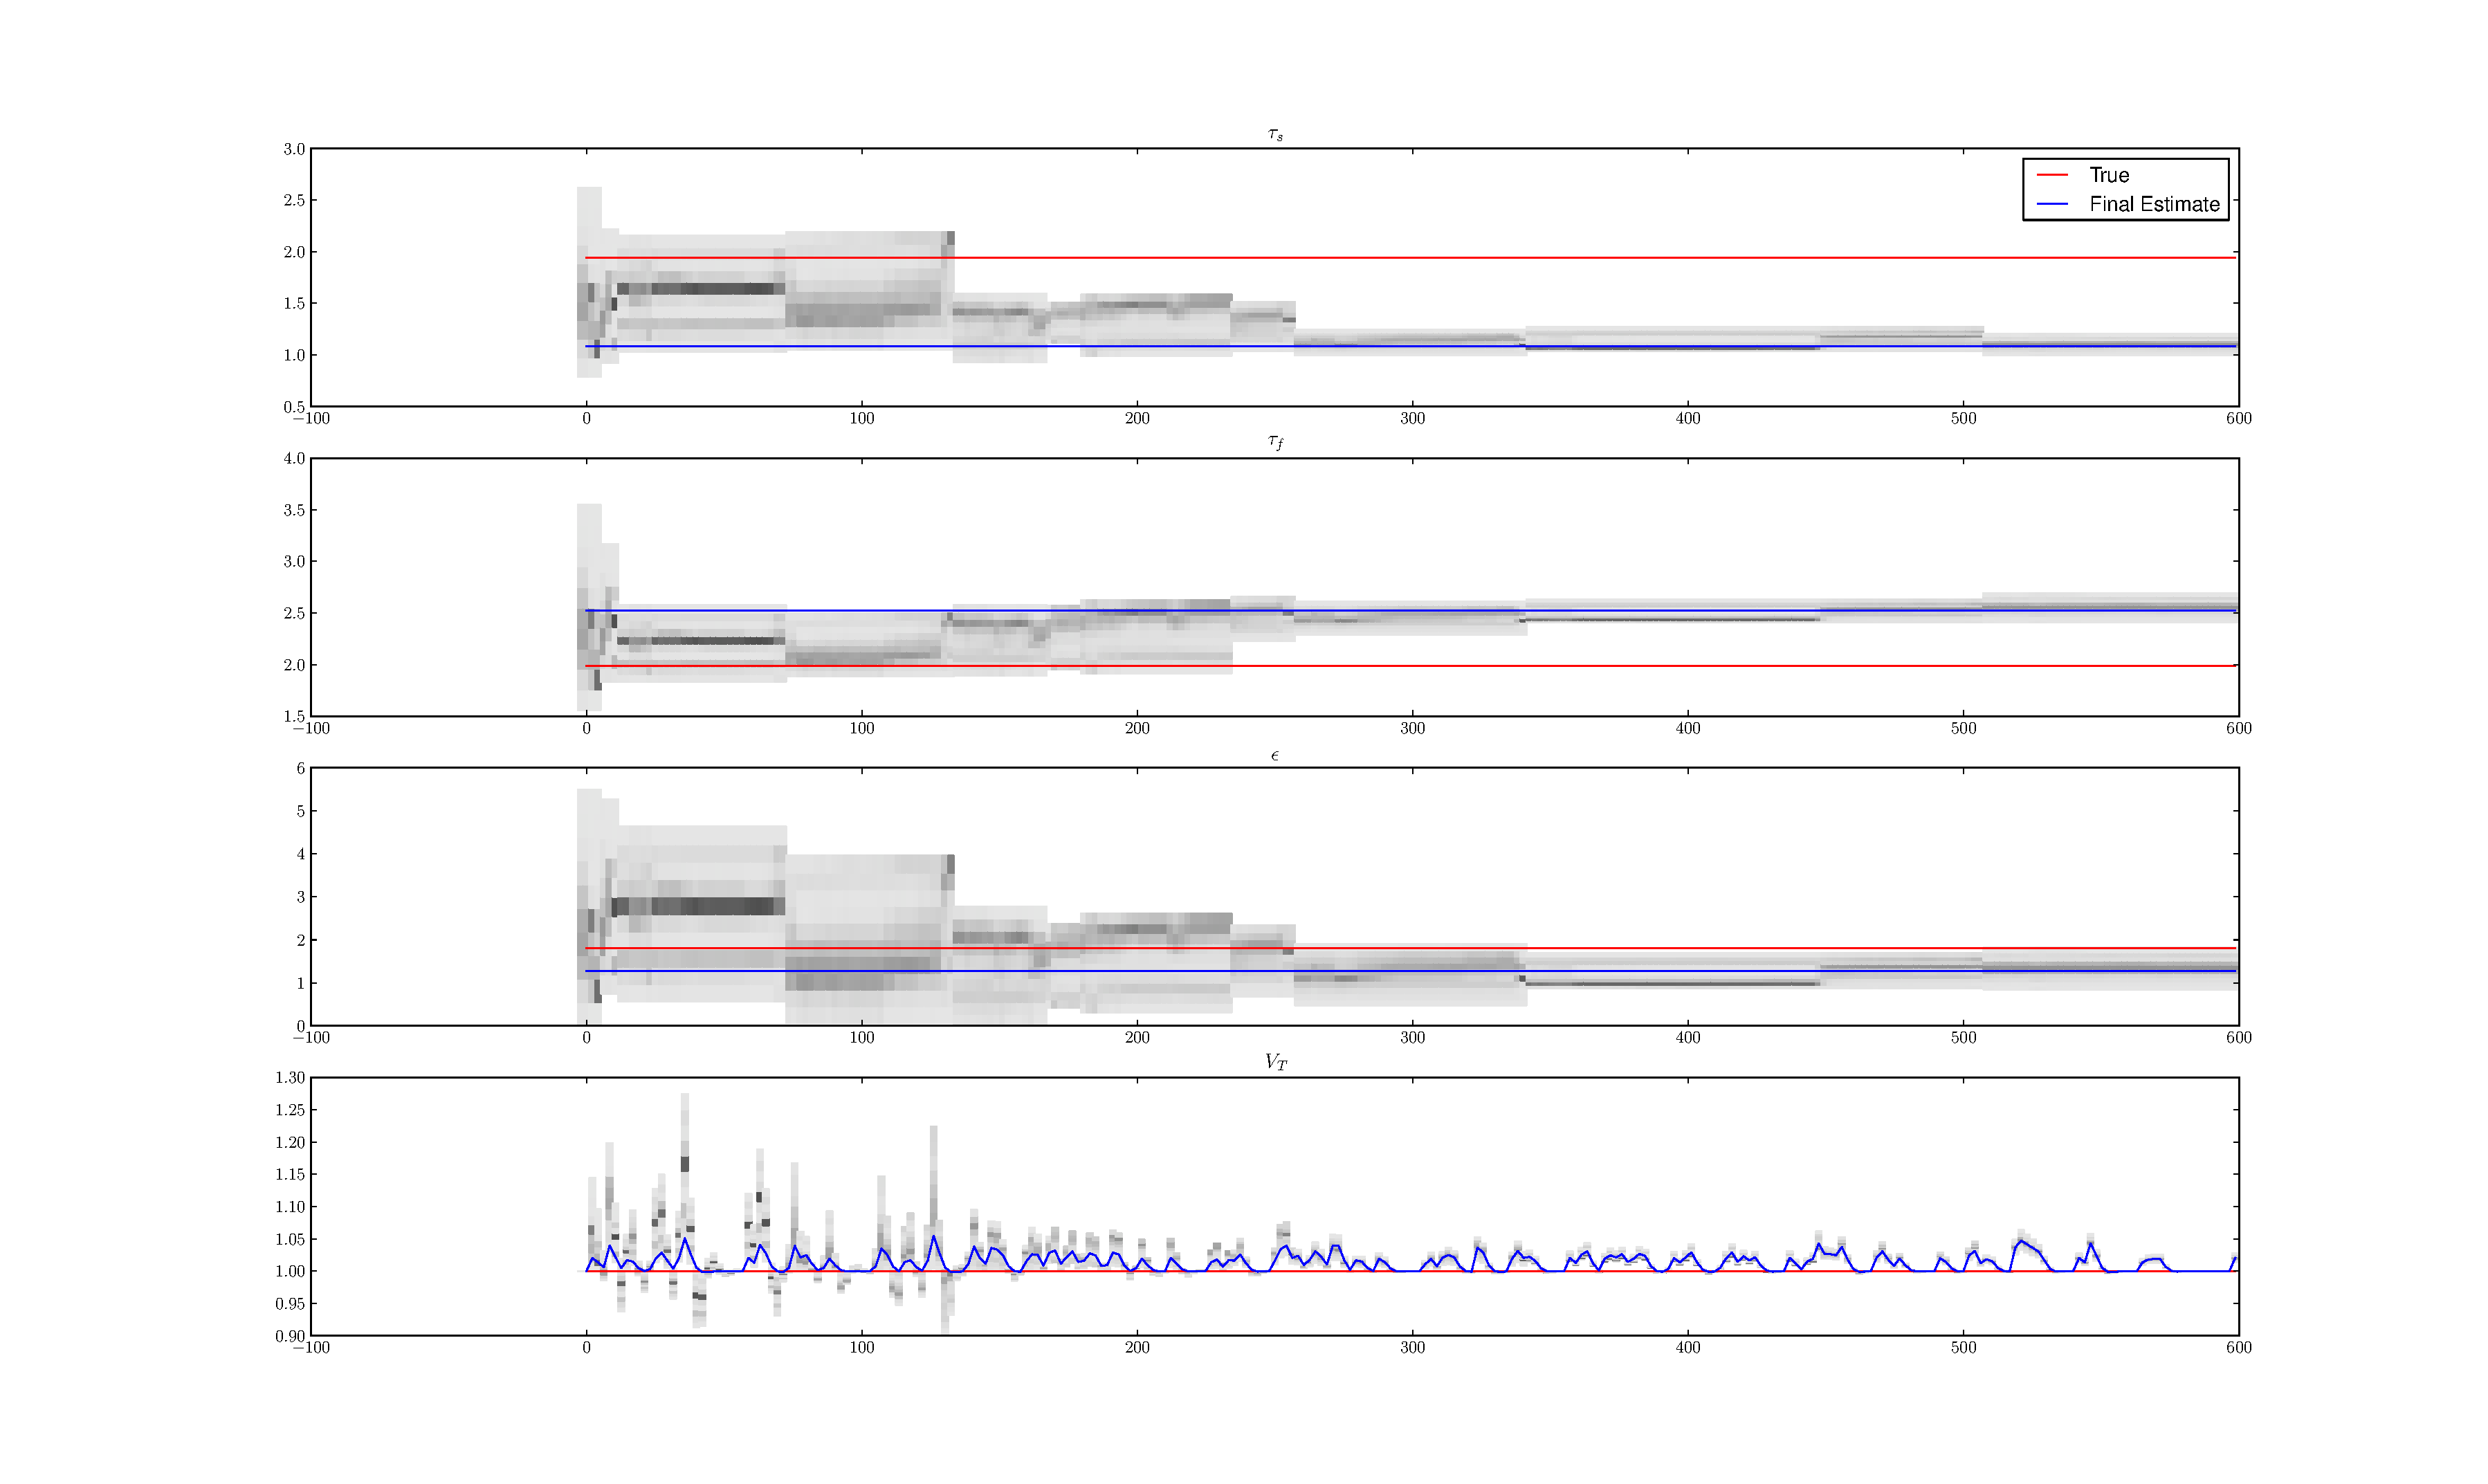
\includegraphics[clip=true,trim=6cm 3cm 6cm 3cm, height=9cm]{images/justbignoise_2}}\\
%\end{figure}
%\begin{figure}[H]
%\subfigure[$q$, $s$, $f$, $BOLD$ ]
%{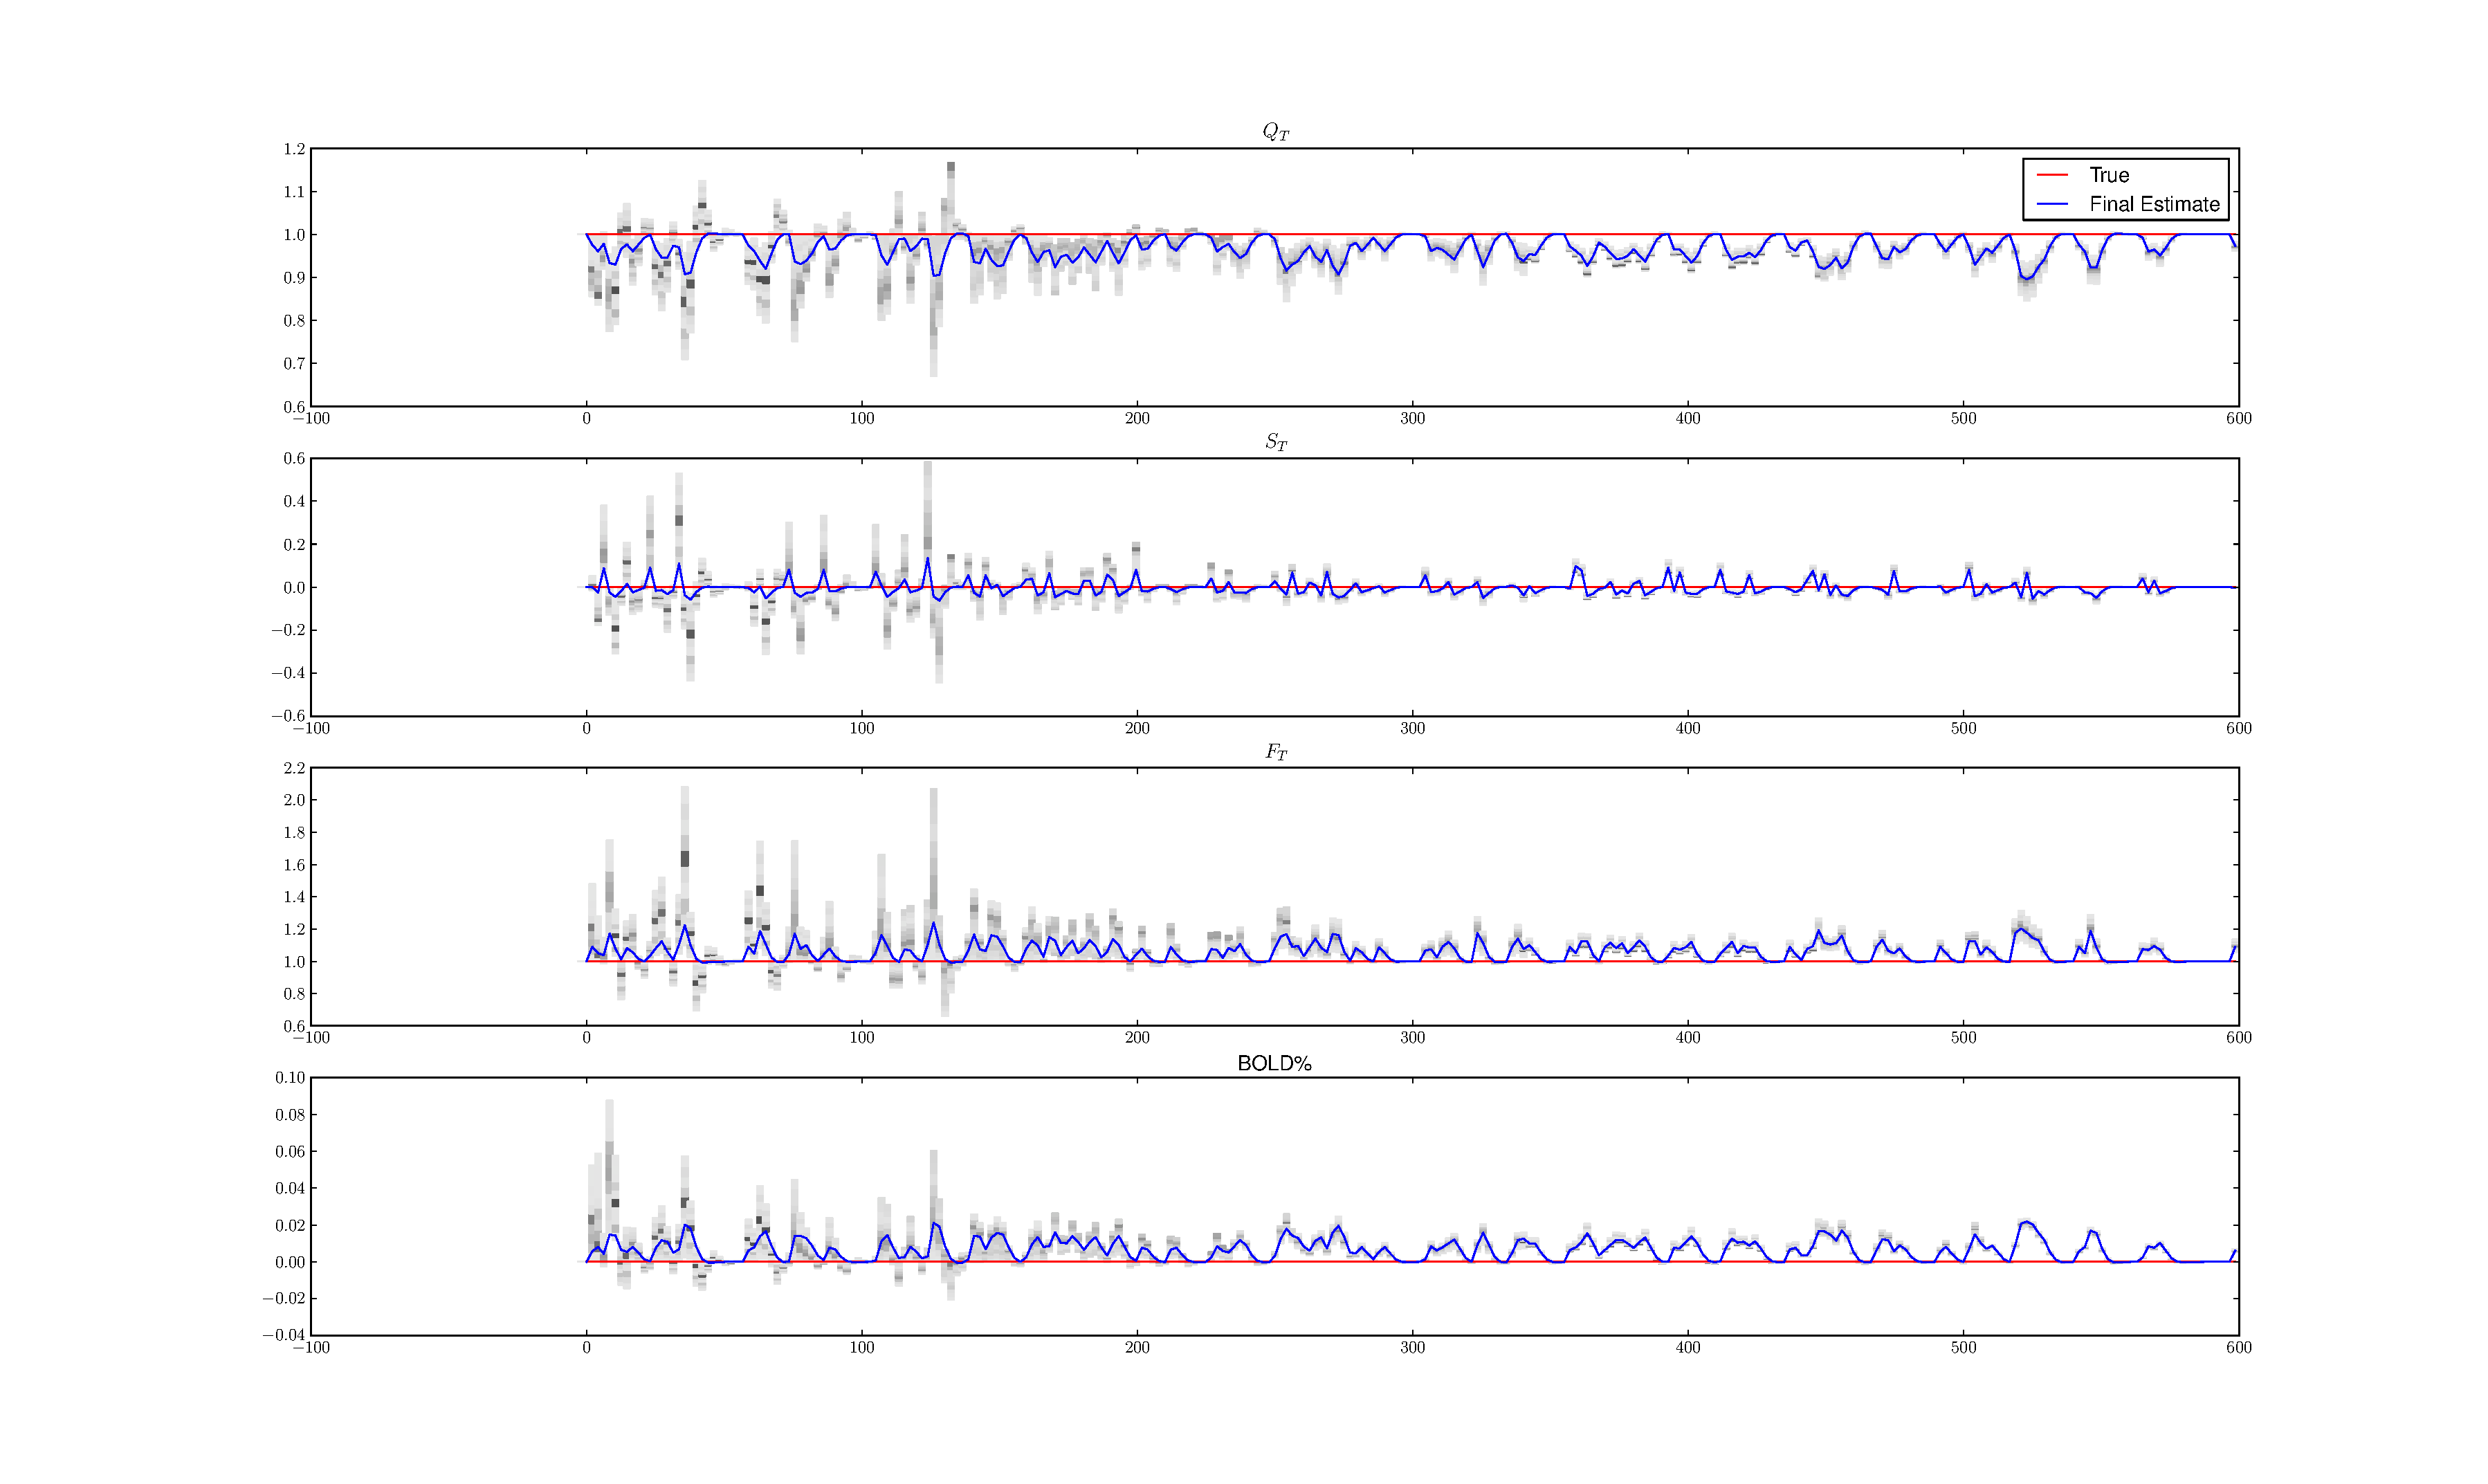
\includegraphics[clip=true,trim=6cm 3cm 6cm 3cm, height=9cm]{images/justbignoise_3}}
%\caption{Converging histogram for parameters when the signal consists purely of noise, with peaks comparable  to
%the convential BOLD signal. ($\sigma_y = .01, \sigma_x = .005$). Same run as fit in \autoref{fig:justbignoise_fit_0}}
%\label{fig:JustNoiseConvergenceLarge}
%\end{figure}

\subsection{Single Voxel Summary}
\label{sec:SingleVoxelReview}
Because of the variability in the signal levels, the
raw \ac{RMSR} cannot be used to rate the fit. As demonstrated by \autoref{tab:NoiseOnlyResults},
a low \ac{RMSR} does not necessarily indicate a good fit.
Therefore, a normalized version of the \ac{RMSR} was used. To normalize the
residual, both the estimated and preprocessed \ac{BOLD} signals were divided by an estimator
of scale and then the new \ac{RMSR} was calculated.
Considering the tendency of \ac{fMRI} to have large unexplainable
peaks and troughs, the Median-Absolute-Deviation (MAD) was used (\autoref{eq:mad}).
This is an estimator of the standard
deviation, and thus a good estimator of the scale of the input signal.
The normalized \ac{RMSR} values are
shown in \autoref{tab:SingleVoxelActivationComparison}. A second potential method of
gauging performance is mutual information. Mutual information is a method of measuring
the interdependence of two random variables. If two signals are truly independent,
then the mutual information will be zero. Although ideally suited to discrete
distributions, by using histograms
it is possible to derive a joint distribution of two signals. The algorithm for
mutual information is based on that joint distribution:
\begin{equation}
\sum_{x,y} p(x,y) \log_2\left(\frac{p(x,y)}{p(x)p(y)}\right)
\end{equation}
Unfortunately the number of bins causes bias in the output, thus to correct for this,
I subtracted the estimated bias:
\begin{equation}
\text{bias} = \frac{N_{bins}}{2Nlog(2)}
\end{equation}
where $N$ is the number of samples and $N_{bins}$ is the number of bins. For all
the mutual information estimates in this work 6 bins were used for the marginal
distribution of each signal. Additionally, throughout log base 2 will be used.
This leads to 36 total bins in the joint, so the bias is:
\begin{equation}
\text{bias} = \frac{18}{N}
\end{equation}
 Note that subtracting the bias can result in negative mutual
information, which should not technically be possible; so any negative mutual information
was taken as 0.

\begin{table}[t]
\centering
\begin{tabular}{|c | c | c | c | c | c | c | c | c |}
\hline
& \multicolumn{4}{|c|}{Signal} & \multicolumn{4}{|c|}{No Signal}\\
\hline
& \multicolumn{2}{|c|}{Low Noise} & \multicolumn{2}{|c|}{High Noise}
& \multicolumn{2}{|c|}{$\sigma_y = 0.001, \sigma_x = 0.0005$}
& \multicolumn{2}{|c|}{$\sigma_y = 0.01, \sigma_x = 0.005$}\\
\hline
& $M.I.$ & N. Res. &
  $M.I.$ & N. Res. &
  $M.I.$ & N. Res. &
  $M.I.$ & N. Res. \\
\hline
\hline
1 &   0.86687  &0.47801 &  0.09077  &1.03894 &  0.06326  &  1.29501 & 0.03024  &1.33641 \\
2 &   0.93975  &0.53177 &  0.13767  &0.95165 &  -0.01075  & 1.30175 & -0.02677 &1.33667 \\
3 &   0.82382  &0.5458  &  0.13505  &0.99539 &  0.02345  &  1.26287 & -0.0111  &1.15957 \\
4 &   0.94661  &0.49824 &  0.04341  &1.16129 &  -0.00906  & 1.43196 & 0.00147  &1.09988 \\
5 &   0.94281  &0.46805 &  0.13718  &1.03972 &  0.00663  &  1.25664 & -0.00204 &1.20107 \\
6 &   0.92539  &0.459   &  0.12337  &1.00214 &  -0.00816  & 1.2708 &  0.01775  &1.04589 \\
7 &   0.98892  &0.46096 &  0.15381  &1.08847 &  0.02664  &  1.15441 & 0.03163  &1.20543 \\
8 &   0.98796  &0.51838 &  0.11325  &1.05962 &  0.03285  &  1.27456 & 0.01951  &1.1225 \\
9 &   0.8804   &0.5253  &  0.09669  &1.0157  &  0.01628  &  1.32024 & 0.01039  &1.08637 \\
10 &  0.88721   &0.49211 & 0.18339  &1.18996 &  0.00407  &  1.34456 & 0.00508  &1.22135 \\
11 &  0.96644   &0.49092 & 0.10949  &0.95368 &  0.03323  &  1.32522 & -0.01284 &1.11737 \\
\hline
mean &0.92329  &0.49714 & 0.12037   &1.04514 &  0.01622  &  1.29437 & 0.00576  &1.17568 \\
\hline
min &  0.82382  &0.459   &  0.04341  &0.95165 & -0.01075  & 1.15441 & -0.02677 &1.04589 \\
\hline
max &  0.98892  &0.5458  & 0.18339   &1.18996 & 0.06326  &  1.43196 & 0.03163  &1.33667 \\
\hline
\end{tabular}
\caption{Mutual Information and the normalized \ac{RMSE}, for each of the previous
sections.}
\label{tab:SingleVoxelActivationComparison}
\end{table}


Comparing the results of \autoref{sec:SimHighNoise} and 
\autoref{sec:PureNoiseHighMag}
in \autoref{tab:SingleVoxelActivationComparison},
distinguishing between these cases with either normalized \ac{RMSR} or 
mutual information is not clear cut. While the average mutual information 
is more than 10 times
the average mutual information in the two non-signal cases, the maximum
mutual information of the low noise/no signal case exceeds the minimum M.I. 
of the high noise/signal
case. The Low Noise/signal determination is easier to make; given
the minimum mutual information is above $.8$ and the maximum normalized 
\ac{RMSR} is below $.6$.
However, it is worth noting that the worst case scenario  for mutual information (maximum) in the
low noise/no signal case does not coincide with the worse case (minimum) normalized residual.
There is no reason why this has to be the case, but it could be beneficial. In
other words, if it were necessary to make a statement that
a particular voxel were active or inactive; the accuracy would improve if both techniques
were used with loose restrictions. In all, both M.I. and the normalized residual
provide a good measure of performance.

There were two primary purposes of these tests. First, given the nature of Monte Carlo
techniques it is important to ensure consistency of results. Although the parameter
sets were inconsistent, the quality of the fit for the \ac{BOLD} output was often
accurate even when noise was drastically increased. The second purpose was to validate
Mutual Information and the normalized \ac{RMSR} as measurements of output quality.
Although not perfect, both methods do provide a decent metric.

\section{Multi-voxel Simulation}
\label{sec:Multi-voxel Simulation}

\begin{figure}
\centering
\subfigure[Region labels for simulated slice.]{
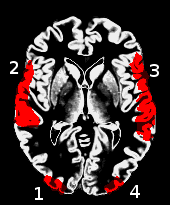
\includegraphics[height=8cm]{images/simregions.png} \label{fig:simslice_mask} }
\subfigure[Normalized \ac{RMSR} Map. Scale is Normalized \ac{RMSE}. Lower (yellow) is better.]
{\label{fig:simslice_hm_res} 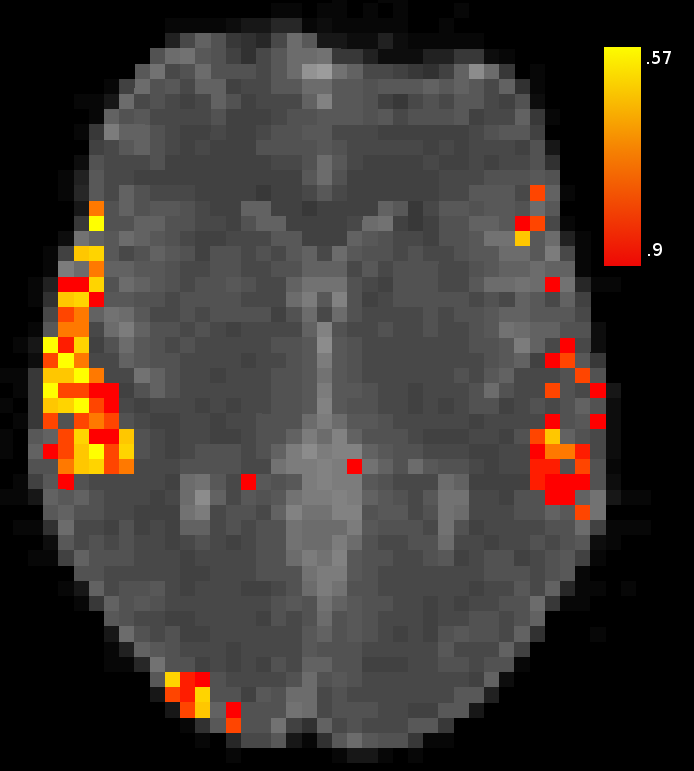
\includegraphics[height=8cm]{images/sim_hm}}
\subfigure[Mutual Information Map. Scale is bits. Higher (yellow) is better.]
{\label{fig:sim_hm_mi} 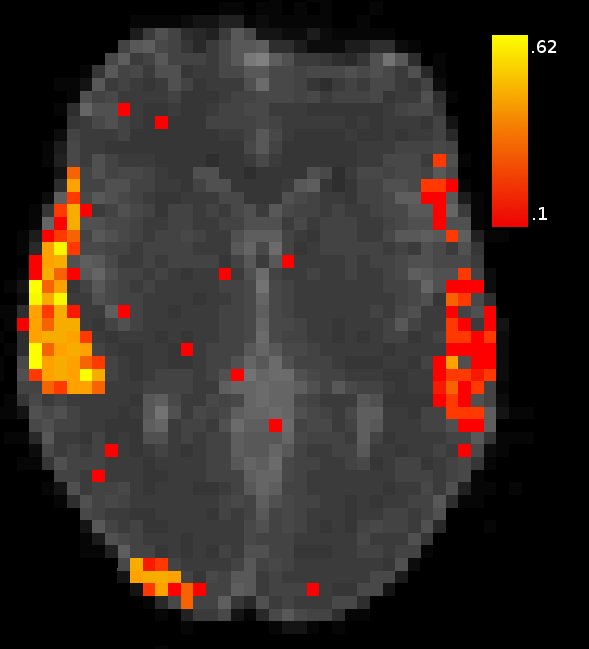
\includegraphics[height=8cm]{images/sim_hm_mi}}
\subfigure[SNR Map of POSSUM simulated data. Mean SNR per region, Region 1: $0.8$, Region 2: $0.97$, and
Region 3: $0.39$.]{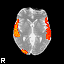
\includegraphics[height=8cm]{images/snr_hm.png}\label{fig:SimSNRhm}}
\caption{Comparison of activation with greymatter, parameter regions.}
\label{fig:simslice_hm}
\end{figure}

To test the usefulness of the particle filter on a larger scale, a modified version
of the FSL tool
POSSUM was used to generate an entire \ac{fMRI} image from a parameter map. The parameter map was generated
by taking an existing activation map and assigning discrete parameter sets to each region.
The result was a four dimensional (length x width
x height x parameter) image with spatially varying parameters. Possum was then modified
to take a parameter map and generate activation levels depending on the parameters at that
point. The patch for POSSUM will be made available. Note that the noise
level was set to an SNR of 20, but due to changes
in the program the true signal-to-noise ratio was much lower, as seen in the
in \autoref{fig:SimSNRhm}. The mean SNR for each region was calculated only for the
voxels with a Signal-To-Noise ratio above $0.1$.

For each time series in the simulated \ac{fMRI} image, the final parameters were saved
into a parameter map. This parameter map could then be compared to the map used to generate the
simulated data. Additionally a new simulation using the calculated parameters could also be
generated to test the difference in \ac{BOLD} levels between the real parameters and the
estimated ones. Since the parameters were far from orthogonal,
 this provided a quantitative difference between the two parameter sets \cite{Deneux2006}.

The regions are numbered according to \autoref{fig:simslice_mask}; the parameters
for each region may be found in \autoref{tab:simsliceparams}.

\begin{table}[t]
\centering
\begin{tabular}{|c |c | c | c | c | c | c | c |}
\hline
Region & $\tau_0$ & $\alpha$ & $E_0$    & $V_0$    & $\tau_s$ & $\tau_f$ & $\epsilon$  \\
\hline
1 & 1.454& 0.321& 0.369& 0.036& 0.994& 2.774& 1.348\\
2 &1.151&  0.353& 0.380& 0.026& 1.98&  2.333& 1.645 \\
3 &1.951&  0.317& 0.348& 0.027& 1.657& 3.719& 0.757 \\
4 &1.203 & 0.310& 0.326& 0.036& 2.168& 2.272& 0.086\\
\hline
\end{tabular}
\caption{Actual parameters for each regions in the simulated slice.}
\label{tab:simsliceparams}
\end{table}

Note that region 4 had a very low $\epsilon$, putting it below the noise
threshold. For this reason, the only areas
with significant estimates of the \ac{BOLD} time series were 1,2 and 3.
Notice that the
regions 1, 2 an 3 stick out in both the \ac{RMSR} and the mutual information
map, indicating that the particle filter was successful in matching those regions.
Mutual information was an extremely successful metric, with the exception of
a few false positives (\autoref{fig:simslice_hm_res}). 
\autoref{fig:sim_hm2} shows what the heat map looks
like when the threshold is raised from $0.1$ to $0.15$.
\begin{figure}
\centering
\subfigure{
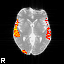
\includegraphics[width=10cm]{images/sim_hm_15_6.png}}
\subfigure{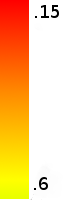
\includegraphics[width=1cm]{images/scale6.png}}
\caption{More stringent mutual information heatmap. Higher (yellow) is better.}
\label{fig:sim_hm2}
\end{figure}

\begin{figure} %bottom left
\centering
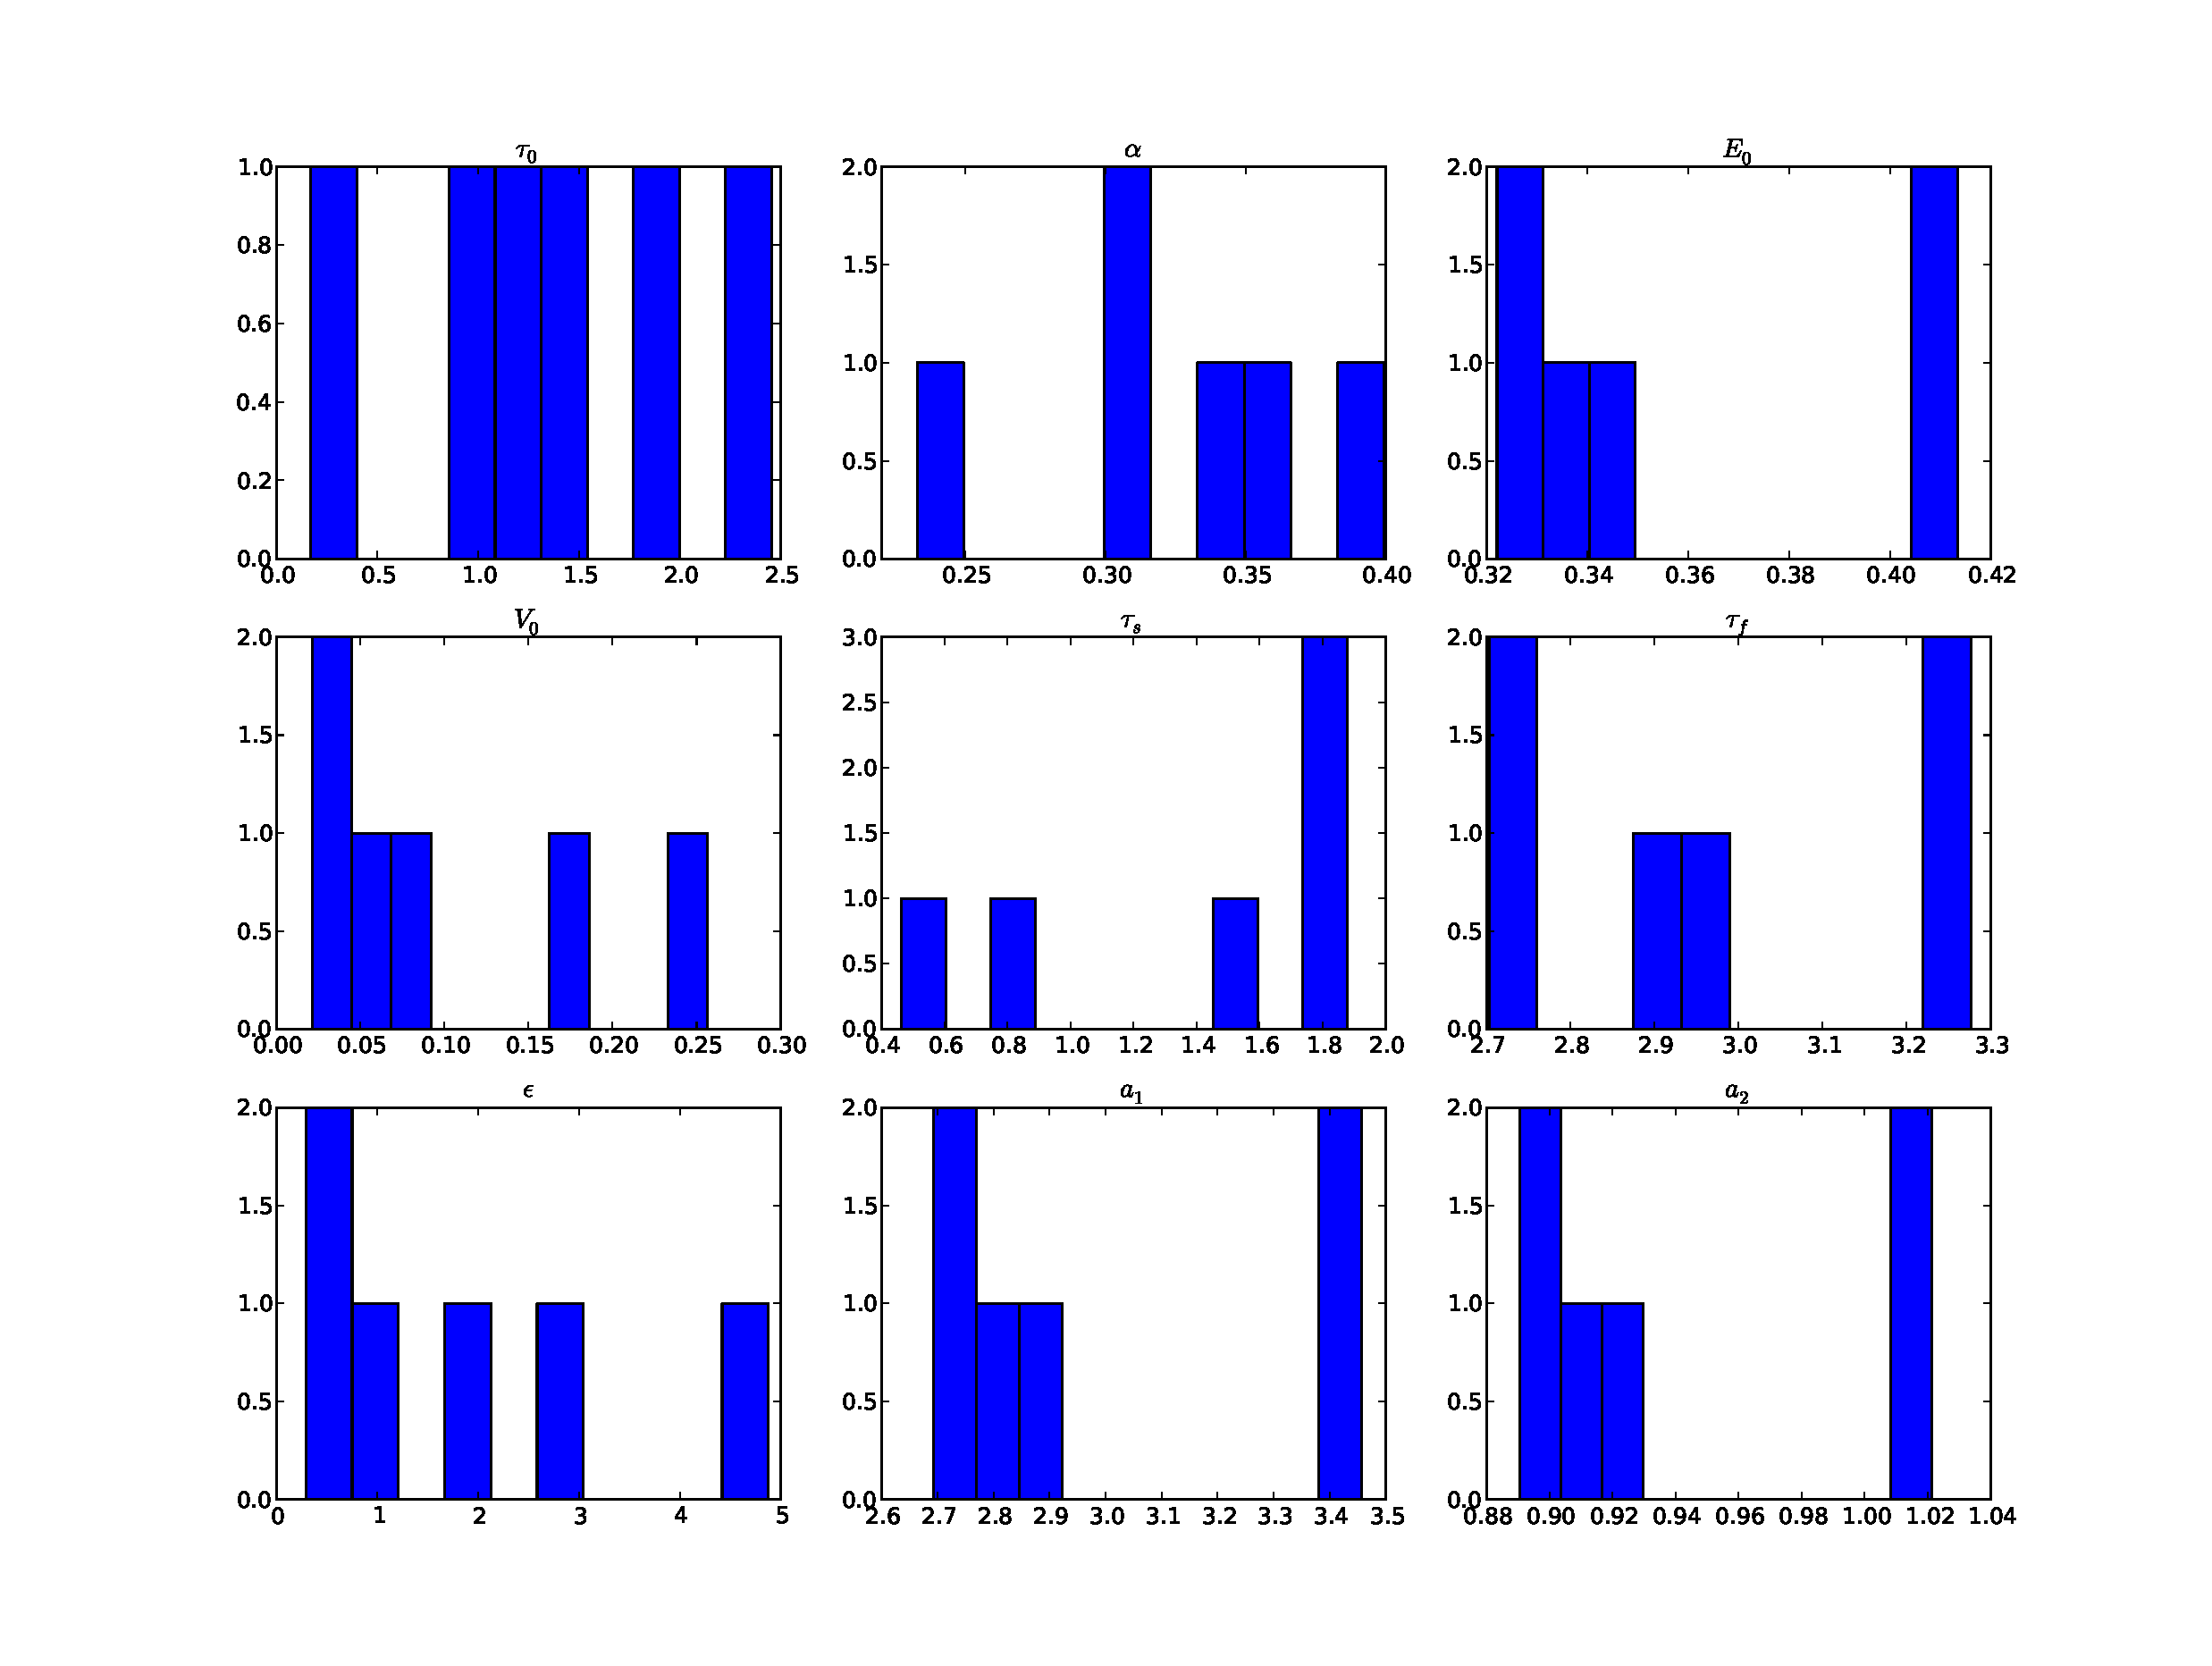
\includegraphics[clip=true,trim=2.5cm 2cm 2cm 1cm,width=15cm]{images/slicesim_hist1}
\caption{Histogram of estimated parameters in section 1 in voxels 
with mutual information greater than $0.15$} \label{fig:slicesim_hist1}
\end{figure}

\begin{figure} %top left
\centering
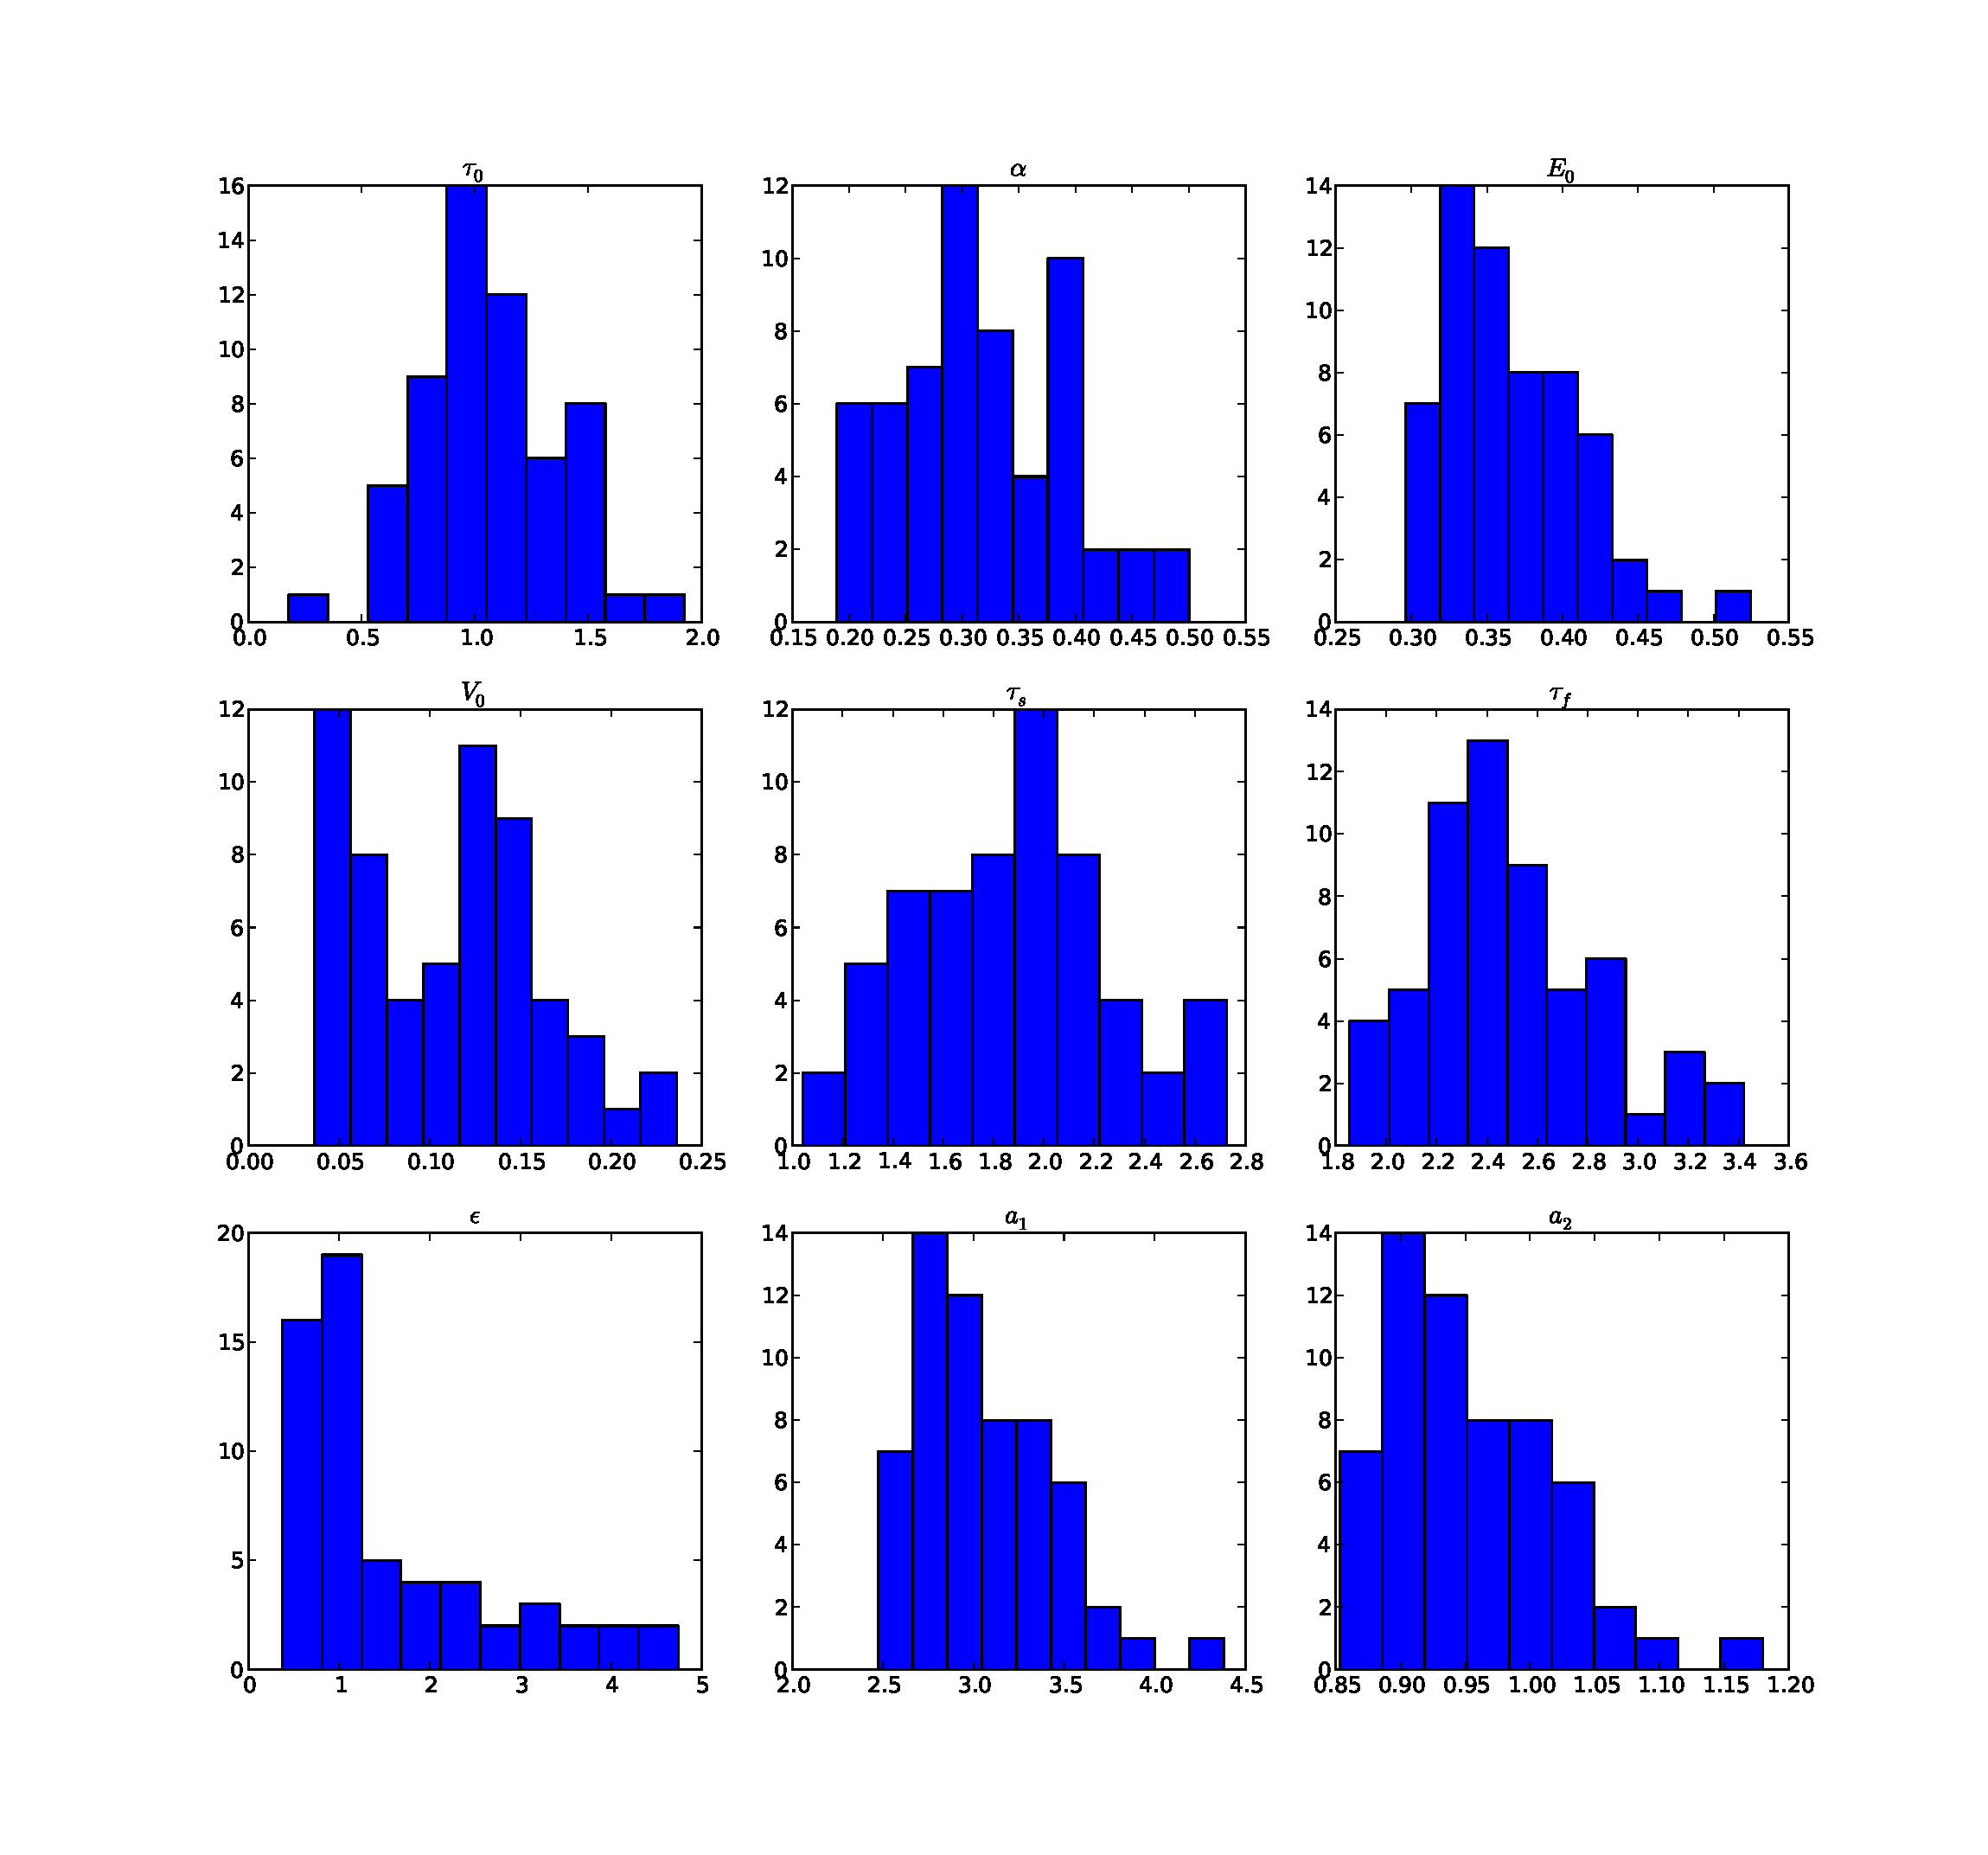
\includegraphics[clip=true,trim=2.5cm 2cm 2cm 1cm,width=15cm]{images/slicesim_hist2}
\caption{Histogram of estimated parameters in section 2 in voxels with mutual information greater
than $0.15$}
\label{fig:slicesim_hist2}
\end{figure}

\begin{figure} %top right
\centering
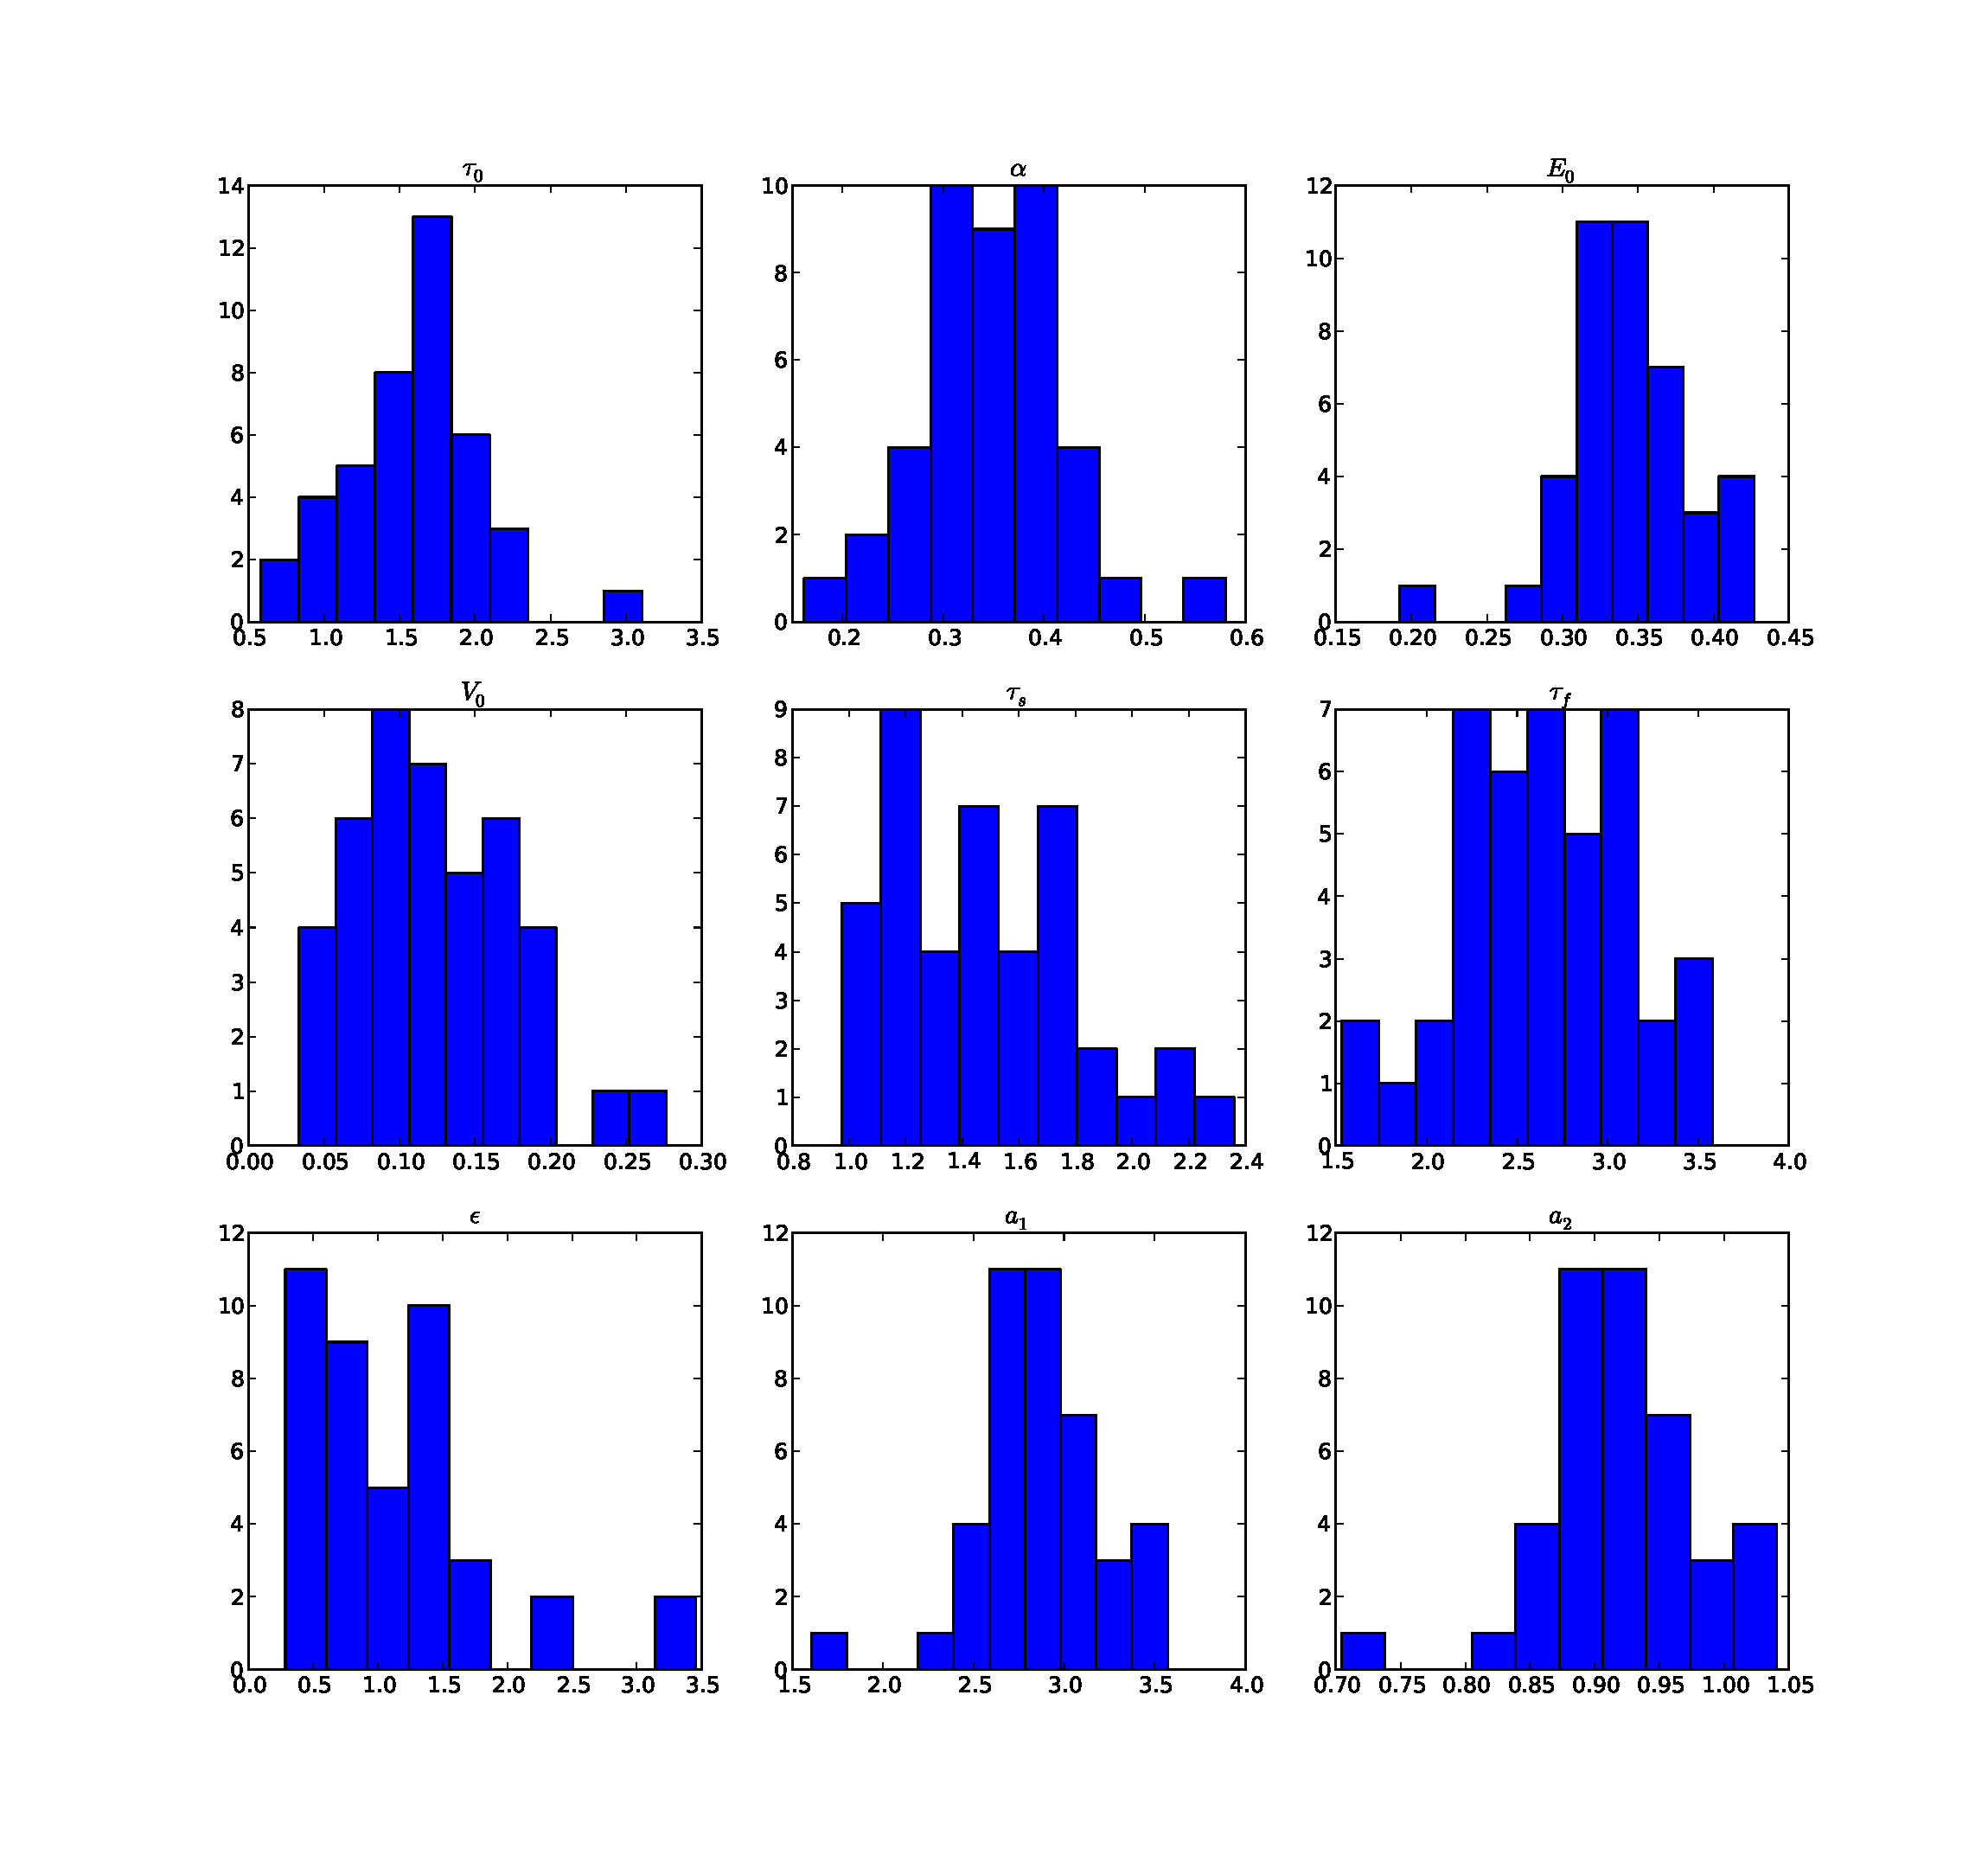
\includegraphics[clip=true,trim=2.5cm 2cm 2cm 1cm,width=15cm]{images/slicesim_hist3}
\caption{Histogram of estimated parameters in section 3 in voxels with mutual information greater
than $0.15$}
\label{fig:slicesim_hist3}
\end{figure}

If the thresholds are left at the values of \autoref{fig:simslice_hm}, then
the normalized \ac{RMSR} gave $2/1479$  false positives and mutual information gave
$11/1479$. However, normalized \ac{RMSR} also clearly missed some active voxels, although
false negatives are harder to quantify because of the presence of white matter.
Raising the threshold to $0.15$ eliminated the false positives in the
Mutual Information map, although some active voxels were also removed.

The histograms again demonstrate that a single point estimate of the parameters
is elusive for this set of parameters. However the data clearly show the power
of the particle filter at identifying regions of activation.
The thresholds applied to this slice, both for mutual information and
\acp{RMSR} are arbitrary. Applying a
threshold is helpful for visualization but is rarely useful for further analysis.
As noted in \autoref{sec:SingleVoxelReview},
the false positives present in the Mutual Information
map are different from those in the \ac{RMSR} map. This furthers the argument
for combining the two metrics to increase power. Although
at first glance it would appear that there are false negatives in
\autoref{fig:sim_hm_mi}; this is
not actually the case. POSSUM simulates different tissues, and white matter
does not typically  have a \ac{BOLD} response. This explains some of the 
holes in regions
2 and 3. These results certainly indicate that the particle filter is effective
at regressing against a noisy signal.
